% ------------------------------------------------------------------------
% ------------------------------------------------------------------------
% ICMC: Modelo de Trabalho Acadêmico (tese de doutorado, dissertação de
% mestrado e trabalhos monográficos em geral) em conformidade com 
% ABNT NBR 14724:2011: Informação e documentação - Trabalhos acadêmicos -
% Apresentação
% ------------------------------------------------------------------------
% ------------------------------------------------------------------------
% Opções: 
%   Qualificação          = qualificacao 
%   Curso                 = doutorado/mestrado
%   Situação do trabalho  = pre-defesa/pos-defesa (exceto para qualificação)
%   Versão para impressão = impressao
\documentclass[mestrado, pre-defesa]{packages/icmc}

% ---------------------------------------------------------------------------
% Pacotes Opcionais
% ---------------------------------------------------------------------------
\usepackage{diagbox}
\usepackage{lscape}
\usepackage{rotating}           % Usado para rotacionar o texto
\usepackage[all,knot,arc,import,poly]{xy}   % Pacote para desenhos gráficos
% Este pacote pode conflitar com outros pacotes gráficos como o ``pictex''
% Então é necessário usar apenas um dos pacotes conflitantes
\newcommand{\VerbL}{0.52\textwidth}
\newcommand{\LatL}{0.42\textwidth}
% ---------------------------------------------------------------------------


% ---
% Informações de dados para CAPA e FOLHA DE ROSTO
% ---
% Tanto na capa quanto nas folhas de rosto apenas a primeira letra da primeira palavra (ou nomes próprios) devem estar em letra maiúscula, todas as demais devem ser em letra minúscula.

% \tituloPT{Profundidade de campo estendida em imagens multifocais de microscopia de luz por meio de técnicas no domínio de transformadas}

% \tituloEN{Extended depth of field in multifocal light microscopy images with transform domain techniques}

\tituloPT{Fusão adaptativa em imagens de microscopia de luz adquiridas em diferentes planos focais}

\tituloEN{Adaptive fusion of light microscopy images acquired in different focal planes}

\autor[Catanante, V. A. A.]{Victor Augusto Alves Catanante}
\genero{M} % Gênero do autor (M = Masculino / F = Feminino)
\orientador[Orientador]{Prof. Dr.}{João do Espírito Santo Batista Neto}
\coorientador{Prof. Dr.}{Odemir Martinez Bruno}
\curso{CCMC}
\data{15}{02}{2019} % Data do depósito
\idioma{EN} % Idioma principal do documento (PT = português / EN = inglês)
% ---


% ---
% RESUMOS
% ---

% Resumo em PORTUGUÊS
% conter no máximo 500 palavras
% conter no mínimo 1 e no máximo 5 palavras-chave
\textoresumo[brazil]{}{}


% resumo em INGLÊS
% conter no máximo 500 palavras
% conter no mínimo 1 e no máximo 5 palavras-chave
\textoresumo[english]{}{}


% ----------------------------------------------------------
% ELEMENTOS PRÉ-TEXTUAIS
% ----------------------------------------------------------

% Inserir a ficha catalográfica
% \incluifichacatalografica{tex/pre-textual/ficha-catalografica.pdf}

% DEDICATÓRIA / AGRADECIMENTO / EPÍGRAFE
% \textodedicatoria*{tex/pre-textual/dedicatoria}
% \textoagradecimentos*{tex/pre-textual/agradecimentos}
% \textoepigrafe*{tex/pre-textual/epigrafe}

% Inclui a lista de figuras
\incluilistadefiguras

% Inclui a lista de tabelas
\incluilistadetabelas

% Inclui a lista de quadros
% \incluilistadequadros

% Inclui a lista de algoritmos
% \incluilistadealgoritmos

% Inclui a lista de códigos
% \incluilistadecodigos

% Inclui a lista de siglas e abreviaturas
\incluilistadesiglas

% Inclui a lista de símbolos
\incluilistadesimbolos


% ----
% Início do documento
% ----
\begin{document}
% ----------------------------------------------------------
% ELEMENTOS TEXTUAIS
% ----------------------------------------------------------
\textual

% \chapter{Introduction}
% \label{chapter:introduction}
% The microscope is a device that performs extremely important tasks to human knowledge, in theoretical or empirical aspects. It is capable of to providing magnified views of small objects and structures. Currently, several variations of microscopes are broadly used, which allows us to investigate much smaller spaces than those visible to the naked eye \cite{wu2008microscope}.

Microscopes are broadly used. In biology, areas such as physiology, histology, taxonomy, cytology and molecular biology stand out. Interdisciplinary fields such as materials sciences also apply microscopy, and health professionals use them in large scale for practical procedures, clinical analysis and research. High throughput microscopy is an important technique for the diagnosis and treatment of genetic diseases. However, to make it acceptable in the clinical environment, it is of great importance to perform high-resolution image acquisition, since low levels of sharpness can directly affect the diagnostic accuracy \cite{qiu2013evaluations}.

The advances in microscopy technologies and methods currently show a natural trend of interdisciplinary research with image processing. This bond dates back to the middle of the 20th century, when some techniques for capturing and manipulating images, primarily developed for televisions, could be
applied to microscopy images \cite{wu2008microscope}. A classic example is noise reduction, which is an important step for cryoelectronic microscopy and also for energy filtering in transmission electron microscopy, before the 3D reconstruction process on \sigla{CT}{Computed Tomography} scans. High noise levels hinder the necessary alignment in the reconstruction task \cite{vyas2017multiscale}.

\section{Motivation}

Biological and biomedical analysis procedures performed using microscopy images also employ image processing algorithms to obtain better results. In this sense, the concept of focus is an element of great relevance. The microscopically analyzed surfaces and structures are \emph{a priori} smooth and homogeneous to the naked eye; when magnified, these images show that those elements are irregular, i.e. they have different depths (when considering an upper view), textures and topologies. It is therefore necessary to constantly adjust the focus to get the image with the least amount of noise and lower frequency of blurred. Figure \ref{fig:ctenanthe} illustrates the problem of differences in depth of focus in a histological image of a \emph{Ctenanthe oppenheimiana} specimen. The focus was adjusted to the greenish central region comprised between the ribs (white band) of the leaf; so the effect of blur was kept on the ribs and their surroundings.

\begin{figure}[htb]
	\centering
	\caption{\label{fig:ctenanthe}Example of a microscopy image with sharpness problem due to focus adjustment.}
	\begin{center}
	    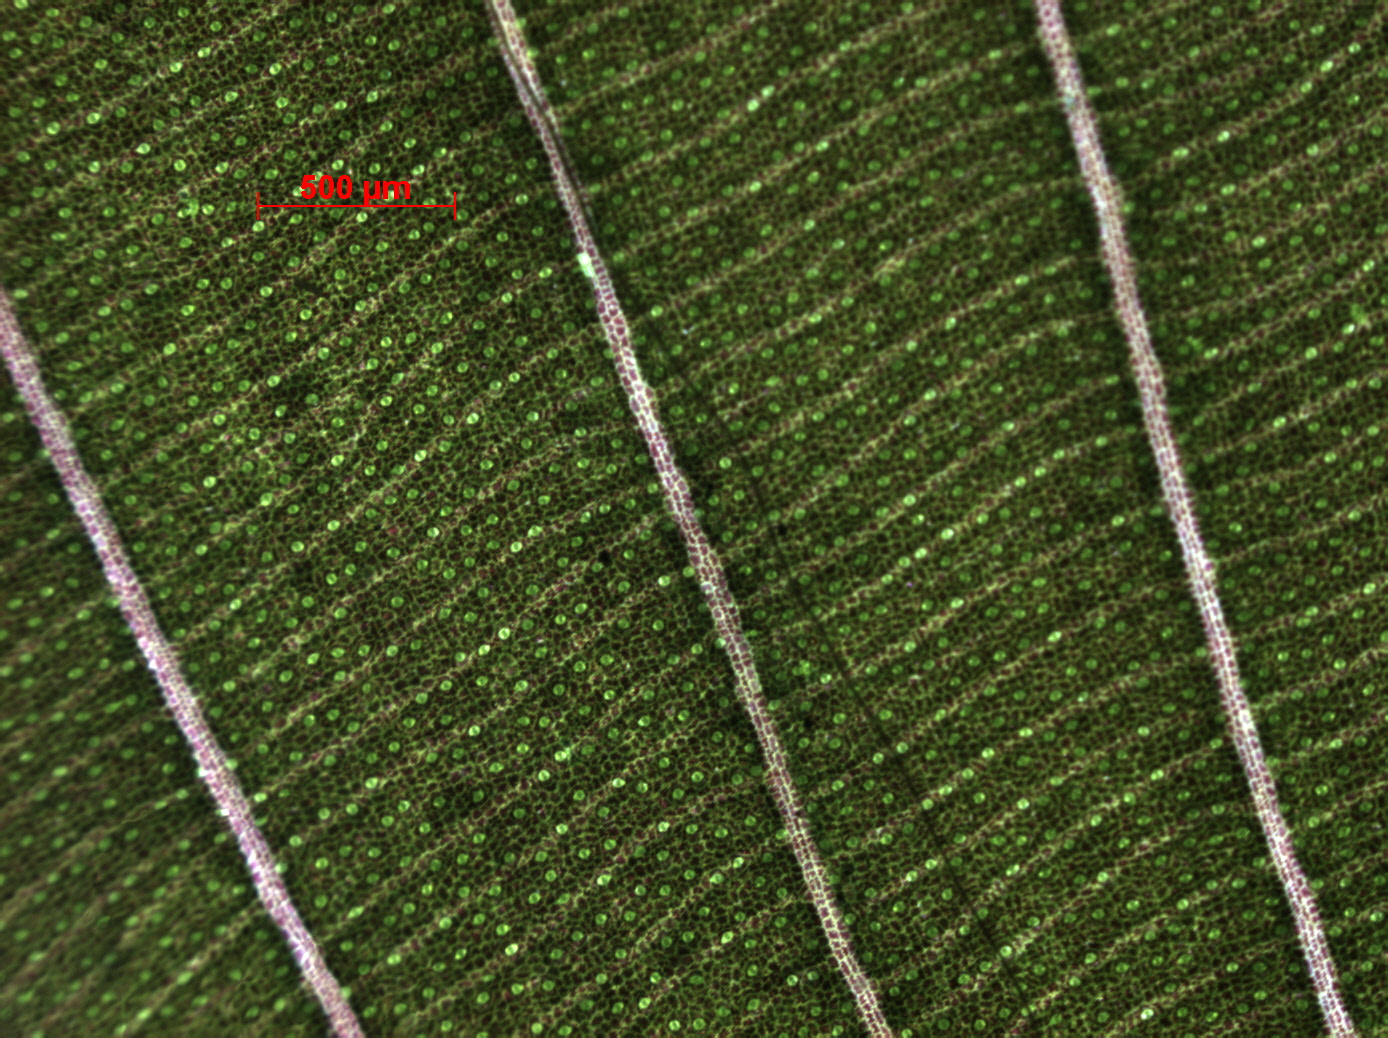
\includegraphics[scale=0.3]
			{images/fig1.png}
	\end{center}
	\centering
	\fautor
\end{figure}

There are several proposed methods to solve the sharpness problem in microscopy images, mostly based on image restoration techniques. According to \citeonline{ponti2016image}, the most frequently used iterative method in microscopic image restoration is the Richardson-Lucy algorithm. This is a particular case of the Maximum Likelihood Expectation Maximization algorithm with spectral extrapolation properties, which assists in the execution process at low conditions of \sigla{SNR}{Signal-to-Noise-Ratio}. Some examples presented by \cite{sun2005autofocusing} consist of
four classes: \emph{derivative algorithms}, \emph{statistical algorithms}, \emph{histogram-based algorithms} and \emph{intuitive algorithms}. Among these applications, derivative methods deserve more credit. The Fourier Transform proved itself to be
effective for low or moderate noise levels; in highly noisy environments, the resulting images were not satisfactory \cite{richardson1972bayesian}. From this evidence, probabilistic methods based on the Bayes Theorem were developed and provided images with better contrast, higher bandwidth and
edge enhancement for confocal fluorescence microscopy samples \cite{ponti2016image}.

The resulting images from such restoration processes have a higher degree of sharpness than the original ones when validated with metrics such as the \sigla{RMSE}{Root Mean Squared Error} and the \sigla{PSNR}{Peak Signal-to-Noise-Ratio} (both will be discussed further). However, the algorithms contain limitations when it comes to degradation as input; consequently, it produces degradation as output. An alternative to restoration is to use images from the same object, with different foci, in order to obtain an enhanced depth of field image with low degradation levels.

\section{Objectives and Hyphothesis}

The objective of this work is to develop a method which is capable of generating an extended depth of field image from a set of light microscopy images, acquired with different foci. The method will employ blur segmentation techniques and image fusion. The specific objectives are described as follows:

\begin{itemize}
    \item \emph{Evaluation of Blur Segmentation Methods}: Several approaches will be described to find the blur map, which employ different segmentation techniques. The aim is to find the approach that has the best behavior with multifocal light microscopy images. Based on current state-of-the-art literature, empirical results of efficiency and efficacy of the methods will be pursued, and a specific method for light microscopy will be developed. The performance evaluation relates to execution time, asymptotic complexity and blur map accuracy;
    
    
\end{itemize}

It is hypothesized that methods based on the Fourier and Wavelet Transforms may be employed to produce a reliable blur segmentation, in order to perform the multifocus image fusion and obtain an extended depth of field image.

\section{Structure of the document}

This monograph is organized as follows:

\begin{itemize}
    \item Chapter \ref{chapter:fundamentals-of-optics-and-light-microscopy} provides several essential concepts of Optics for understanding the Light Microscopy basics and the nature of blur;
    
    \item Chapter \ref{chapter:image-processing} contains the theoretical background in image processing, necessary for the comprehension of the related work and the proposed methods;
    
    \item Chapter \ref{chapter:related-work} apply the image processing basis and some other concepts with the most related relevant work in blur segmentation and multifocus image fusion areas;
    
    \item Chapter
    \ref{chapter:materials-and-methods} exposes details of the proposed approaches for solving the problem;
    
    \item Chapter \ref{chapter:preliminary-results}
    show some experimental results with artificially blurred images and real microscopy multifocus images;
    
    \item Chapter \ref{chapter:conclusions} is designed in this period for presenting the schedule of what should be done next in order to achieve the objective and use this work to contribute to science.
    
\end{itemize}


\chapter{Fundamentals of Optics and Light Microscopy}
\label{chapter:fundamentals-of-optics-and-light-microscopy}
Microscopes are instruments designed to accomplish several important tasks to human knowledge, either in the theoretical or the empirical domains. They are capable of magnifying images of small objects and structures, which otherwise would not be seen by the human eye; this grants more information about the object of study to the research or the analysis. The first idea of the device was introduced by Romans, which discovered the magnifying property of glass in some sort of biconvex shape. Zacharias Janssen (1588-1632) was responsible for the invention of the first compound microscope with a concave eyepiece and  Francisco Fontana (1580-1656) introduced the convex eyepiece version of it \cite{zilio2009optica}. Furthermore, Robert Hooke (1635-1703) and Anton van Leeuwenhoek (1632-1723) were the most prominent science-related men responsible for microscope improvements \cite{wu2008microscope}.

Science is subject to continuous technological improvements that reflect on every field of study. Due to the development of theories and their empirical proofs of veracity, in addition to the advances in hardware and software power, techniques such as image processing are relentlessly applied to other fields. This also happens in microscopy, aiming to improve image quality, data reliability, and range of use \cite{boyde1990modern}.

This chapter provides important information about light microscopy and optics, with regards to the project's scope. The first part is dedicated to the basic set of concepts and properties from optics that are necessary for light microscopy; the second one describes the structure of the optical microscope, along with its uses and implications on the acquired images. Plenty of image degradation is due to the system acquisition process; in fact, defocus is a natural occurrence in optics, mainly caused by adjustments of the optical system.

\section{Relevant elements of optics}

The definition of the spectroscopy procedure consists of the interaction between electromagnetic radiation and the matter \cite{gauglitz2006handbook}. This concept can be extended to microscopy, which deals with the section of the electromagnetic spectrum of wavelength comprehended between 400 and 700 nanometers, i.e. visible light,  to create visual representations of the objects
\cite{bell2009introduction}. Light microscopy is inherently related to optics, and some concepts of the field are directly related to the blurring process; therefore, it is meaningfully important to elucidate them.

\subsection{Dual Nature of Light}

The light was described in different ways according to different geniuses. Isaac Newton (1642-1727) proposed that light had a corpuscular nature, due to the trajectory in which light appeared to travel in a uniform medium in his experiments; Christiaan Huygens (1629-1695) stated in his works that light was traveling in a "wave-like" way and apparently could explain some optical principles such as the interference phenomena \cite{fowles1989introduction}. 

The corpuscular approach for explaining the behavior of light was accepted during the 17th and 18th centuries since Newton played a central role in science in that era. The development of electricity and magnetism as solid fields of research and theoretical representations of natural phenomena was happening concomitantly with optics. Michael Faraday (1791-1867) connected magnetism and light for the first time with his studies on light polarization in magnetic field immersed materials. Later, James Clerk Maxwell (1831-1879) established a complete relation between optics and electromagnetism by defining the displacement current density - a relation that involves the polarization of a medium, the intensity of electric fields and the electric permittivity of vacuum - and writing its differential equations \cite{zilio2009optica}.

Light as an electromagnetic wave is therefore composed of the two vectors and propagates in some particular coordinate direction upon a metric space, e.g. the $\mathit{x}$ coordinate on a three-dimensional Euclidean space. Hence, it is possible to treat light as a wave or particle, according to the application or needs. Light microscopy deals with light as a wave and its related phenomena such as reflection, refraction, interference and diffraction, which will be presented on the following subsections and are useful for a deeper understanding of this work. Posterior studies of Max Planck (1858-1947), Albert Einstein (1879-1995) and Niels Bohr (1885-1962) \cite{fowles1989introduction} linked the prior discoveries with the quantum theory, and therefore differ from this research's scope. Maxwell enunciated that there were two different vectors which could cause a state of disturbance in the space while dealing with electric charges; those consist of the electric vector $\mathit{\mathbf{E}}$ and the magnetic induction vector $\mathit{\mathbf{H}}$. Together, they construct the electromagnetic field \cite{born1999principles}, as shown in \autoref{fig:electromagnetic_wave}.

\begin{figure}[htb]
	\centering
	\caption{\label{fig:electromagnetic_wave} 
		Composition of the electromagnetic wave. The red and the blue curves represent the electric and induction vectorial quantities, respectively.}
	\begin{center}
	    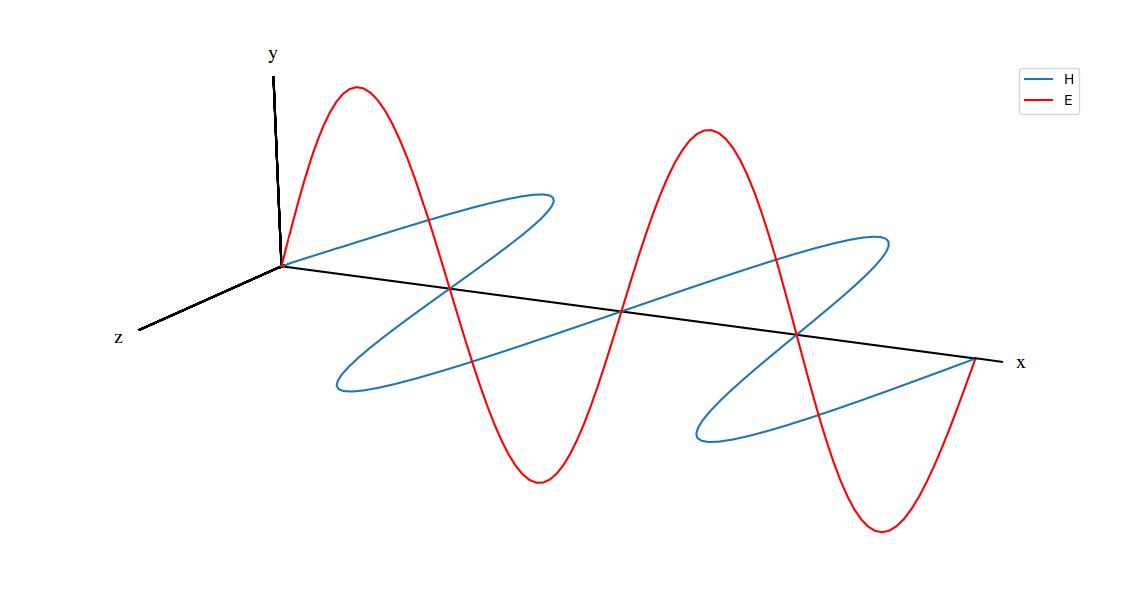
\includegraphics[scale=0.3]
			{images/fig2.png}
	\end{center}
	\centering
	\fautor
\end{figure}

\subsection{Light Wave Properties and Phenomena}

The light waves can be represented by a ray, i.e. a single oriented line which shows the direction of propagation; several waves that propagate in nearly the same direction can be named as a beam \cite{halliday2013fundamentals}. These two models of the real light are important and useful representations within the boundaries of visible light, and allow easier explanations of light properties. Some basic properties of waves are important for a full understanding of optical phenomena related to microscopy and its image formation, and may be described according to \citeonline{tipler2007physics} as follows:

\begin{itemize}
    \item \emph{Frequency}: The number of cycles per unit of time, or the reciprocal of the time that a periodic wave takes to execute a complete cycle of oscillatory motion, given by $f = \frac{1}{T}$;
    
    \item \emph{Amplitude}: The maximum displacement from the equilibrium position, where the wave peak reaches its highest value;
    
    \item \emph{Phase}: A point in time on the cycle of a wave propagation, quantified in degrees.
\end{itemize}

Rays or beams of light may come from a picometric scale source (due to nuclear processes) or from a relatively larger scale, e.g. the fluorescent and incandescent light bulbs, which are sources of electric light. Eventually, light reaches surfaces during its propagation, and this is the event that allows the human vision sense; when it occurs, there are four prominent phenomena to consider: reflection, refraction, interference and diffraction. The incident ray of light suffers a split procedure when it reaches a frontier between two homogeneous media. One of the resulting rays propagates in the initial medium and the other one propagates inside the other medium; the first phenomenon is denominated \emph{reflection} and the second, \emph{refraction} \cite{born1999principles}.

The speed of light depends on the medium in which it propagates. The \emph{refractive index} is a number that quantifies the speed of light in a particular medium in relation to the speed of light a vacuum, and can be described by

\begin{equation}
    \label{eqn:refractive_index}
       n = \frac{c}{v},
\end{equation}

\noindent where $\mathit{c}$ is the speed of light in vacuum and $\mathit{v}$ is the speed of light in the medium. According to \citeonline{halliday2013fundamentals}, the reflection law states that the resulting ray propagates within the incidence plane and that the angle of reflection $\mathit{\theta^{'}_{1}}$ equals the $\mathit{\theta_{1}}$ angle of incidence; comparably, the refraction law states the same about the incidence plane and relates the incidence $\mathit{\theta_{1}}$ and refraction $\mathit{\theta_{2}}$ angles by Snell's law, given by

\begin{equation}
    \label{eqn:snells_law}
       n_{2}\sin{\theta_{2}} = n_{1}\sin{\theta_{1}},
\end{equation}

\noindent where $\mathit{n_{1}}$ and $\mathit{n_{2}}$ are the refractive indices of the media. This framework consists of an approximation and may be considered ideal for didactic purposes. The process that happens in the real situations may involve non-homogeneous media, opaque or translucent media (which blocks the propagation of light or randomly changes the direction of the rays, respectively), and those concepts are relevant to the imaging procedures, e.g. microscopy. \autoref{fig:beam_split} depicts the real-world phenomenon and its ideal representation.



\begin{figure}[htb]
	\centering
	\caption{\label{fig:beam_split} 
	    (a) Example of a beam of light that reflects and refracts when touching the frontier between air and water. (b) Representation of the process with rays.}
	\begin{center}
	    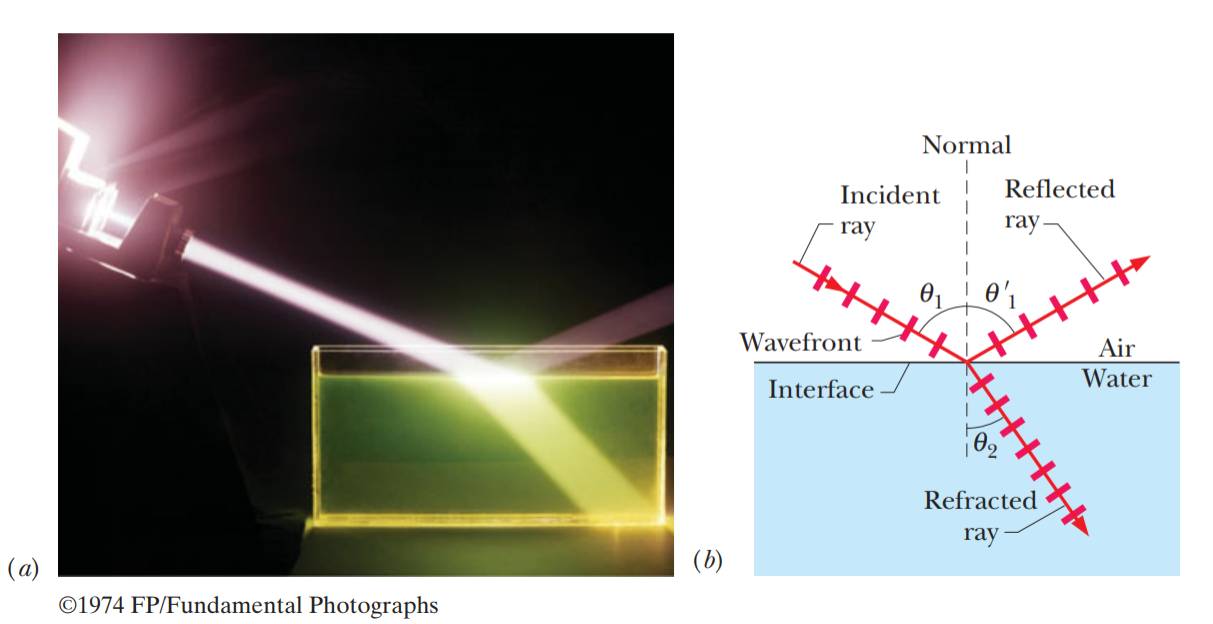
\includegraphics[scale=0.3]{images/fig3.png}
	\end{center}
	\centering
    \fdireta{halliday2013fundamentals}
\end{figure}

When two or more waves of similar or equal frequency superpose in space and form of a different intensity pattern, it is said that the \emph{interference} of the waves occurred \cite{tipler2008physics}. Mathematically, when interference is observed with light waves, it consists in a vector addition of the electromagnetic fields \cite{zilio2009optica}.
If the interfering waves are in phase, i.e. the difference between the same positions within the wave cycles of the two waves is zero. This process is called \emph{constructive}, which yields a larger amplitude to the new wave. Similarly, if the interfering waves are not in phase, then the process is named \emph{destructive} and yield smaller or null amplitudes to the new wave \cite{tipler2007physics}. Both types of interference are show in \autoref{fig:interference}.

\begin{figure}[htb]
	\centering
	\caption{\label{fig:interference} 
	    (a) Constructive interference and (b) destructive interference.}
	\begin{center}
	    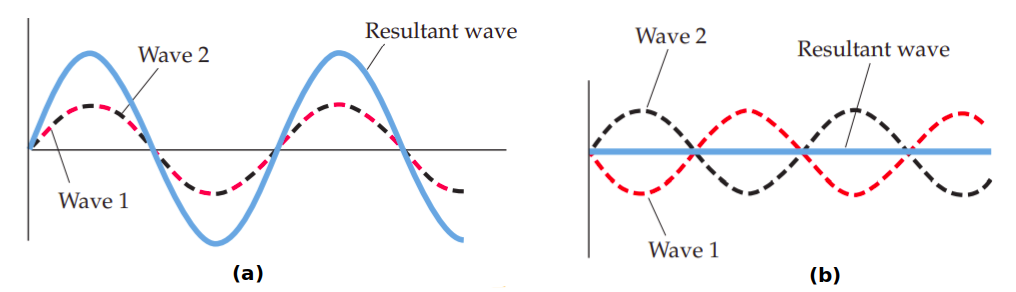
\includegraphics[width=\textwidth,height=5cm]{images/interference.png}
	\end{center}
	\centering
    \fadaptada{tipler2007physics}
\end{figure}

The wave theory of light also contains another important property for the real processes: the \emph{diffraction}, a phenomenon that was discovered by Francesco Maria Grimaldi (1618-1663) and consists of the distortion in a wavefront which focuses on obstacles such as apertures on an object, spheres, disks, or anything with similar dimension to the wavelength of the focusing light \cite{zilio2009optica}. The wavefront deviates and scatters after propagating through the obstacle and transforms itself into circular or spherical waves; this is a relevant property that distinguishes a wave from a particle, since the latter would either propagate without any change in its trajectory or would be blocked by the obstacle \cite{tipler2007physics}. When a beam of light reaches an opaque object, the waves suffer changes in their direction of propagation, which can be predicted by the fact that all the points in each wavefront (points of identical phase on waves) generate a new wave, as stated by Huygens \cite{fowles1989introduction}. As described by the Huygens principle, each point of the wavefront acts as a source and creates secondary waves which scatter in every direction; each of the new wavefronts is generated by the interference of an infinite number of sources of waves \cite{zilio2009optica}. The scheme in \autoref{fig:diffraction} illustrates the diffraction phenomenon with an arbitrary obstacle and a small source of waves.

\begin{figure}[htb]
	\centering
	\caption{\label{fig:diffraction} Diffraction scheme of a wavefront.}
	\begin{center}
	    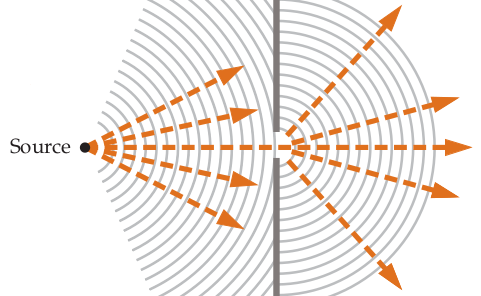
\includegraphics[scale=0.5]{images/diffraction.png}
	\end{center}
	\centering
    \fdireta{tipler2007physics}
\end{figure}

Diffraction is a phenomenon that always happens as waves pass through apertures, but its magnitude depends on the relative proportions between the aperture size and the wavelength: when the latter is large in comparison to the former, the diffraction effects are large and, likewise, a relatively small wavelength yields smaller effects \cite{tipler2007physics}. As stated by \citeonline{zilio2009optica}, there are two common types of diffraction:

\begin{itemize}
    \item \emph{Fresnel Diffraction}: also named near-field diffraction, it occurs when a cylindrical wavefront (the curvature cannot be neglected) passes through an obstacle and diffracts in the near-field, i.e. short distances relative to the path of the diffracted waves' propagation. Practically, the observation distance is finite. It results in different sizes and shapes for the diffraction patterns;
    
    \item \emph{Fraunhofer Diffraction}: also named far-field diffraction, it occurs when planar waves (the curvature of the wavefront may be neglected) pass through an obstacle in the far-field, i.e. large distances relative to the path of the diffracted waves' propagation. Practically, the observation distance is infinite. It results in different sizes for observed aperture images.
    
\end{itemize}


\subsection{Illumination Qualities}

The propagating waves, rays or beams of light that illuminate the object in imaging systems carry some attributes which depend on the source and the desired result. \autoref{fig:illumination_qualities} depicts some relevant qualities of light. 


\begin{figure}[htb]
	\centering
	\caption{\label{fig:illumination_qualities} Comparison between different qualities of an imaging systems' illumination setup.}
	\begin{center}
	    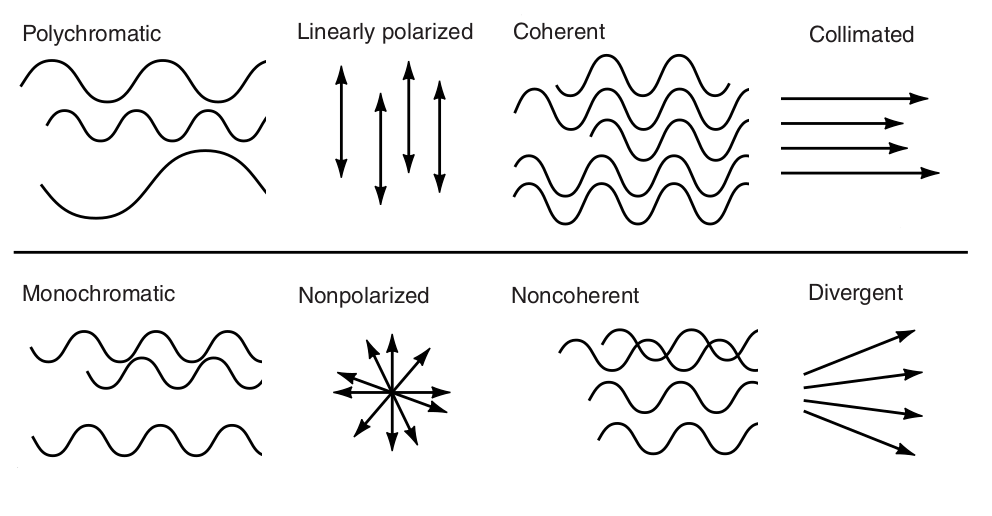
\includegraphics[scale=0.4]{images/light_qualities.png}
	\end{center}
	\centering
    \fadaptada{murphy2012fundamentals}
\end{figure}

Pursuant to \citeonline{murphy2012fundamentals}, the attributes in \autoref{fig:illumination_qualities} 
refer to:

\begin{itemize}
    \item Color: every ray in a \emph{monochromatic} beam has the same wavelength, i.e. the same color. Similarly, \emph{polychromatic} or simply colored beams consists of a mixture of rays with different wavelengths;
    
    \item Polarization: vibration in the electric vector of light as an electromagnetic wave may occur
    in parallel planes or not. The latter characterizes \emph{polarized light} and the former, \emph{nonpolarized light};
    
    \item Coherence: relationship between the phase of each wave of a given wavelength. If the phase is the same for all waves, as in a laser beam, the light is named \emph{coherent}. If phases are not the same, than it is said that the illumination is \emph{noncoherent} or \emph{incoherent}, as in bright-field microscopes;
    
    \item Direction: The waves may propagate in parallel trajectories, i.e. be \emph{collimated}, or may diverge or converge to some point.
    
\end{itemize}

\subsection{Properties of the Spherical Lenses}
Within the scope of this work, the main reason for introducing the concepts of optics is the imaging devices - the microscope, in particular. The structure of the apparatus will be described in Section \ref{sec:light_microscopy}. Moreover, a substantially large amount of devices rely on optical lenses for imaging, with properties such as depth of field and depth of focus.

As stated by \citeonline{halliday2013fundamentals}, \emph{lenses} are objects consisting of a transparent material, with a certain refractive index, that are made of two spherical surfaces on which light propagates and suffers refraction. They are used in optical systems due to their capacity to create images as long as their refractive index is not equal to that of the medium. Still, in agreement with \citeonline{halliday2013fundamentals}, some concepts related to lenses are important in our context and will be shown below. The following list depicts the principal elements from geometric optics that relates to lenses and its consequent imaging properties:

\begin{itemize}
    \item \emph{Radius of Curvature}: the distance between the center of the sphere and a refracting surface, named $\mathit{r_{1}}$ and $\mathit{r_{2}}$ on Figure \ref{fig:spherical_lens};
    
    \item \emph{Center of Curvature}: since the lenses are made by a union of two sections of a sphere-shaped object (which have a center), there are two Centers of Curvature for each lens, denoted by $\mathit{C_{1}}$ and $\mathit{C_{2}}$ on Figure \ref{fig:spherical_lens};
    
    \item \emph{Central Axis}: a line that represents the infinite number of radii of the sphere, which contain the center and the focal point;
    
    \item \emph{Focal Point}: also called \emph{focus}, a point within the central axis, where the image of the object is formed due to the convergence of the light rays from the object, and shown on Figure \ref{fig:spherical_lens} as $\mathit{F_{1}}$ and $\mathit{F_{2}}$;
    
    \item \emph{Focal Length}: presented as $\mathit{f}$ on Figure \ref{fig:spherical_lens}, it stands for the distance between the center of the sphere and the focal point;
    
    \item \emph{Object}: either a point or a surface on space that emits (or reflects) light and can be interpreted as a source;
    
    \item \emph{Image}: in this context, it is a representation of an object, formed by the action of lenses.
    
    \item \emph{Magnification}: a number that describes how larger or smaller the image will be in comparison to the object; mathematically, the ratio of the image distance to the object distance, both relative to the lens.
    
\end{itemize}

A single lens or a set of lenses (most of the optical systems are more complicated than a single lens) have the \emph{depth of field} and the \emph{depth of focus} properties. Although the terms appear to be similar, the former relates to objects and the latter, to images \cite{davidson2002optical}. For every system, there is a focal plane in which the formed images will be sharp. Depth of Field is the tolerance for the object focal plane that may produce sharp images, while Depth of Focus dictates the same tolerance for the image focal plane. In other words, depth of field is the zone in the real world that would yield an acceptably sharp image and depth of focus is the same idea for the imaging sensors or for plotting the image.Figure \ref{fig:spherical_lens} denotes an illustration of an arbitrary spherical lens.

\begin{figure}[htb]
	\centering
	\caption{\label{fig:spherical_lens} Arbitrary scheme of the optical properties of a spherical lens.}
	\begin{center}
	    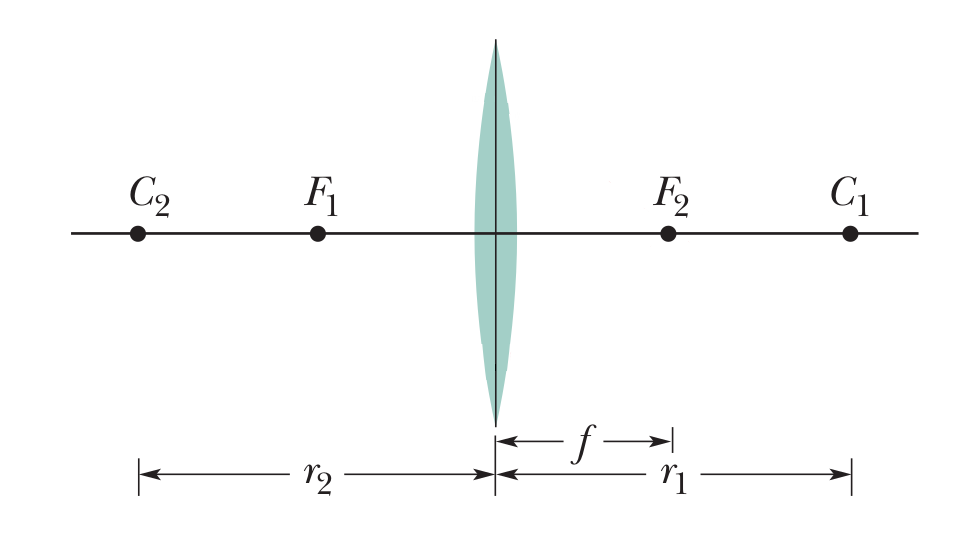
\includegraphics[scale=0.4]{images/fig4.png}
	\end{center}
	\centering
    \fadaptada{halliday2013fundamentals}
\end{figure}

Some properties of the spherical lenses directly influence the image formation process and, consequently, the resulting image quality. The \emph{numerical aperture}, as reported by \citeonline{murphy2012fundamentals}, is a measurement in terms of angles that shows how much lenses can capture light, and is given by

\begin{equation}
    \label{eqn:numerical_aperture}
    NA = n \sin{\theta},
\end{equation}

\noindent where $\theta$ is the half angle of the cone of specimen light accepted by the objective lens and $n$ is the refractive index between the lens and the specimen. There are optical flaws in lenses that hinder a proper image formation. Those are named \emph{aberrations} \cite{lawlor2019introduction}, and the most relevant types in the scope of this project are the \emph{spherical aberrations}. According to \citeonline{murphy2012fundamentals}, the spherical aberrations occur when there is a difference in the focal point of incident parallel rays at central and peripheral locations of a spherical lens' surface, which yields a blurred image of either a point source of light or an extended object. It is possible to correct a spherical aberration by changing the shape of the refracting surface, i.e. changing the radius of curvature for the lenses in order to adjust the focal point to one particular distance \cite{smith1988optics}. The illustration in Figure \ref{fig:spherical_aberrations} represents the spherical aberration for a point source of light, where it is possible to see the difference between incident rays in the borders and in the inner regions of the lens. The resulting image is, in this case, a set of concentric circles around a point.

\begin{figure}[htb]
	\centering
	\caption{\label{fig:spherical_aberrations} Arbitrary example of the spherical aberration.}
	\begin{center}
	    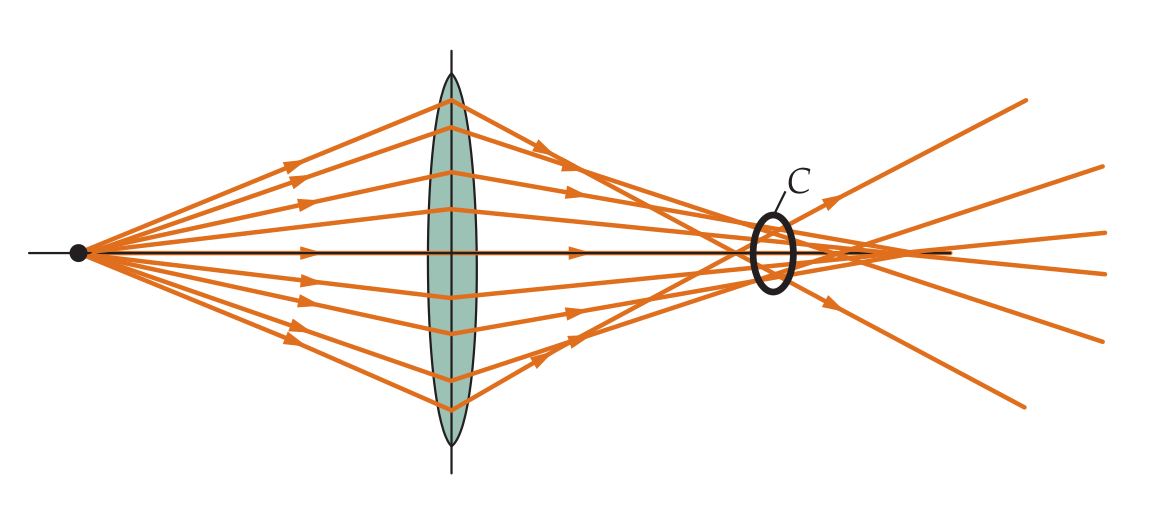
\includegraphics[scale=0.3]{images/spherical_aberration.png}
	\end{center}
	\centering
    \fdireta{tipler2008physics}
\end{figure}


\section{Light microscopy}
\label{sec:light_microscopy}

There are several techniques and approaches for employing optical lenses to obtain magnified images. Especially, in the scope of this work, light microscopy is a simple yet robust example to understand, explore and integrate with image processing techniques. This section presents some concepts and principles of light microscopy, as well as important key definitions for the next chapter.

\subsection{Types of Light Microscopy}

According to \citeonline{dokland2006techniques}, the purpose of light microscopy is to provide magnified images of specimens by means of capturing emitted, reflected or transmitted light in the visible range of the spectrum, or even in the ultraviolet or near-infrared regions. As reported by \citeonline{lawlor2019introduction}, there are three general styles of light microscope. The \emph{upright microscope} is the easily affordable, easy to use traditional configuration with a light source on the base, a stage and the objectives. The \emph{inverted microscope} consists of the same configuration as an upright microscope, but inverted, and offers some advantages when it comes to life sciences applications such as live cell imaging. Finally, the \emph{stereomicroscope}, which is the type of microscope used in this project, is a compound microscope with two eyepieces.

\subsection{General Structure of a Compound Microscope}

Historically, the structure of the first microscopes developed by Hooke and Leeuwenhoek had no eyepiece; the compound microscope, developed by Janssen, consists of the magnification lenses and also an eyepiece, which adds more magnification power and delivers the image to the user \cite{lawlor2019introduction}. As stated by \citeonline{murphy2012fundamentals}, the word \emph{compound} refers to the fact that the objective lens and the eyepiece (or ocular), work together to produce the final magnification of the image as a product of their magnifications. A graphical representation of the general structure of a compound microscope is shown in \autoref{fig:compound_microscope}.

\begin{figure}[H]
	\centering
	\caption{\label{fig:compound_microscope} Graphic representation of the basic compound light microscope structure.}
	\begin{center}
	    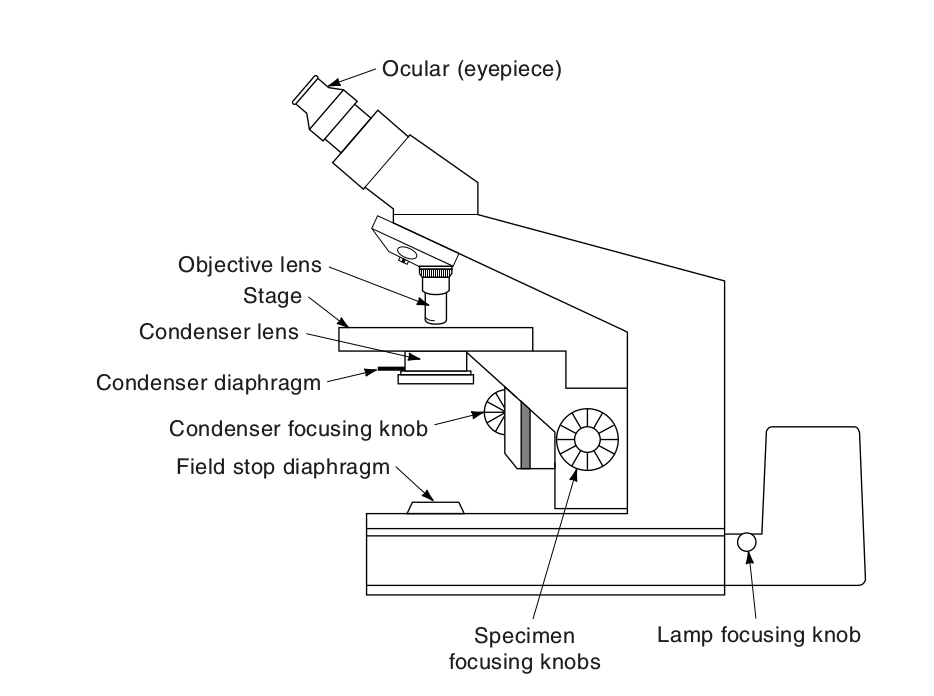
\includegraphics[scale=0.4]{images/fig5.png}
	\end{center}
	\centering
    \fdireta{bell2009introduction}
\end{figure}

As reported by \citeonline{bell2009introduction}, the basic structure of most light microscope models consists of objective lenses, eyepieces, condensers, the stage and the light source. They are described as follows:

\begin{itemize}
    
    \item \emph{Objective Lenses}: a set of multiple lenses merged inside a tubular structure (barrel), which are designed for capturing light rays from the specimen or object and are built for minimizing the series of optical unwanted phenomena in imaging;

    \item \emph{Eyepieces}: lenses where the observer may look through, also inside a tubular structure, but with lower magnification in comparison to the objective;

    \item \emph{Condensers}: a collector of light from the light source, which focus the rays on the object;
    
    \item \emph{Stage}: the support for the object; which may have height and positional adjustments in some devices;
    
    \item \emph{Light Source}: the main source of light, usually a lamp.
\end{itemize}

Since light is some sort of radiation, there are several different ways to achieve imaging in microscopes; it can be made by light, polarized light, lasers, X-rays, among others. There are also advanced techniques such as confocal microscopy, which is capable of imaging a very small area of the object, with all the light rays focused on it \cite{rochow1994introduction}. he choice of the most suitable microscopy depends on the task.

\subsection{Stereo Compound Microscope}

As previously discussed, of the versions of compound microscopes is the stereomicroscope. It consists of a fusion of two compound microscopes in a convergent optical system and may have two different objectives and eyepieces or only one objective and two eyepieces \cite{schreier2004advances}. The former is named \emph{binobjective-binocular} (Greenough) and the latter \emph{monobjective-binocular}, or \sigla{CMO}{Common Main Objective Stereo Microscope}. 

One of the advantages of CMO microscopes is the higher depth of field, which allows the user to view and investigate biological specimens, relatively small materials and any kind of non-smooth surfaces. Furthermore, it is possible to view and acquire images in three dimensions \cite{rochow1994introduction}. The structure of both types of stereo compound microscopes are depicted in \autoref{fig:stereo_compound_microscope}.

\begin{figure}[htb]
	\centering
	\caption{\label{fig:stereo_compound_microscope} Graphic representation of the basic stereo compound light microscope structure, (a) for the Greenough type and (b) for the CMO.}
	\begin{center}
	    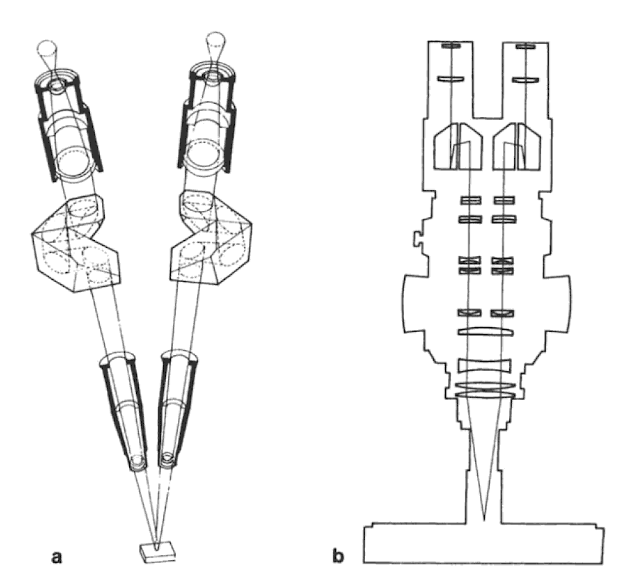
\includegraphics[scale=0.45]{images/fig6.png}
	\end{center}
	\centering
    \fdireta{rochow1994introduction}
\end{figure}


\subsection{Light Microscopy Techniques}
Concerning the use of light microscopes, there are several techniques and configurations which are achieved by varying the amount of lenses and light sources: bright-field, dark-field, phase-contrast, differential interference and fluorescence \cite{roane2009microscopic}. In this work, the \emph{stereomicroscopy}, \emph{bright-field microscopy} and the \emph{z-stacking} procedure are used in order to capture images. As stated by \citeonline{lawlor2019introduction}, the images in bright-field microscopy are characterized by the contrast between the sample and the bright white background, generated by transmitted light. It is commonly used in pathology and histology fields for imaging fixed cells and tissues, showing the structure, shape, and organization of those. The amount of light should be controlled, since the sample might suffer substantial changes, e.g. the chlorophyll molecules when illuminated by UV and visible light suffer irreversible breakdown (photodegradation) generates other photoproducts \cite{petrovic2017clorophyll}. The Figure \ref{fig:bright-field_microscopy} provides an example of bright-field microscopy image.

\begin{figure}[htb]
	\centering
	\caption{\label{fig:bright-field_microscopy} Example of bright-field microscopy of a bone tissue.}
	\begin{center}
	    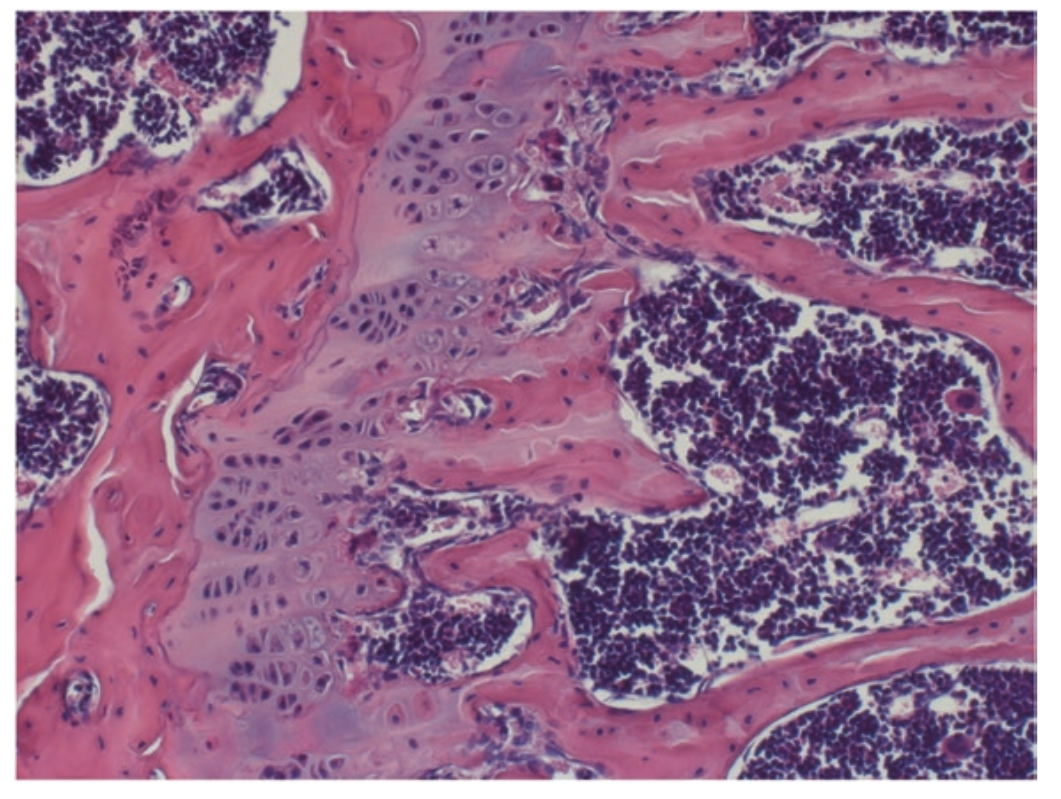
\includegraphics[scale=0.3]{images/bright-field_microscopy.png}
	\end{center}
	\centering
    \fdireta{lawlor2019introduction}
\end{figure}

The z-stacking is a procedure to capture images in different positions concerning the $z$ axis, named slices, which may be applied to many different techniques and creates a pseudo 3D image of the sample and consequently retrieve depth information about the specimen \cite{lawlor2019introduction}. The distance between each slice is determined by how the technique is done, either manually or automatically, and the focus needs to be adjusted at each slice. Later, the images need to be aligned before any analysis. Figure \ref{fig:z-stack_example} represents a z-stacking example.

\begin{figure}[H]
	\centering
	\caption{\label{fig:z-stack_example} Z-stack images of yeast cells, acquired in positions under the focal plane (-15, -10 and -5 $\mu m$), exactly on it (0 $\mu m$) and above it (5, 10 and 15 $\mu m$).}
	\begin{center}
	    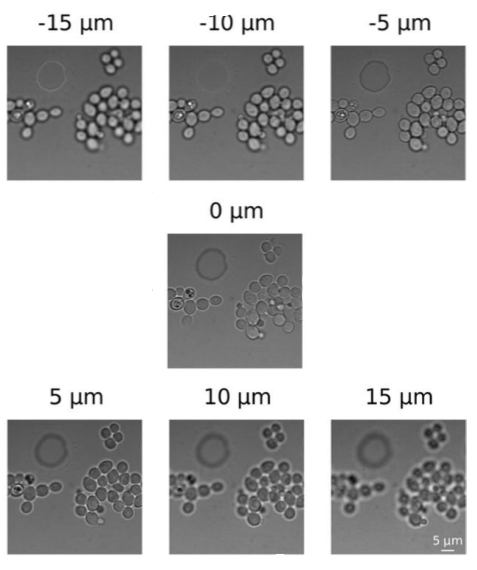
\includegraphics[scale=0.5]{images/z-stack.png}
	\end{center}
	\centering
    \fadaptada{wei2018neural}
\end{figure}

\chapter{Bright-field Microscopy Image Formation and Degradation}
\label{chapter:blur-characterization-and-image-formation}
%%%%%%%% symbols to add
\simbolo{f(x,y)}{Original image as a function of spatial coordinates $x$ and $y$}

\simbolo{g(x,y)}{Observed image as a function of spatial coordinates $x$ and $y$}

\simbolo{J_{1}}{Bessel function of the first kind}

% \simbolo{\eta}{Additive noise function}

% \simbolo{\ast}{Convolution operation}

% \simbolo{\delta}{Dirac delta function}

% \simbolo{\mathbb{R}}{Set of real numbers}

% \simbolo{\mathbb{N}}{Set of natural numbers}

% \simbolo{\wedge}{Diagonal matrix of decrescent multiple singular values}

% \simbolo{\mathbb{G} = (\mathbb{V},\mathbb{E})}{Graph}

% \simbolo{\mathbb{V}}{Set of vertices of a graph}


The human eye constructs images from incident light rays on the \emph{retina}, a very complex set of photoreceptors that converts light into electrical signals which are later interpreted by the brain. The result of this process may be modelled as continuous function of two variables $f(x,y)$ which comprises the \emph{illumination} and the \emph{reflectance} information, i.e. the amount of incident light and the amount of reflected light in the scene, respectively \cite{gonzalez2018digital}.

Digital image processing deals, as the name proposes, with \emph{digital images}, i.e. discrete representations of $f(x,y)$ generated by sensors that are capable of transforming the illumination and reflectance information into electric signals. Still according to \citeonline{gonzalez2018digital}, in order to achieve this representation, the signals undergo sampling (signal conversion from continuous to discrete) and quantization (mapping of real-valued intensities to discrete pixel values) processes. For the sake of notation simplicity, $f(x,y)$ denotes the digital image and the term ``image'' also refer to it along this work.

It is clear that the image formation is influenced by several factors: sensor type, scene illumination conditions, and others. Indeed, each imaging system such as a camera or a microscope adds its own constraints to the process, e.g. conventional transmitted light microscopy images are only achieved with non-opaque samples \cite{rudi2020contrast}. Although there are many types of microscopy with different imaging procedures, this work limits its scope to bright-field microscopy. Therefore, this chapter summarizes the bright-field microscopy image formation processes and its implications on quality of the images. Furthermore, it describes blur properties concerning its origins either in image formation or other events. 

\section{Image Formation}
As mentioned in \autoref{chapter:fundamentals-of-optics-and-light-microscopy}, the bright-field microscopy images are formed by either transmitted or reflected light that passes through the sample and reach the objective lens. There difference between transmitted light and reflected light microscopes is the illumination system; there is no difference in how both direct light rays after those leave the specimen \cite{leng2009materials}.

According to \citeonline{davidson2002optical}, the light which reaches the specimen is either undeviated, i.e. does not suffer any disturbances in its direction, or diffracted; the diffracted rays leave the sample with a phase difference of 180 degrees in comparison to the undeviated light and cause destructive interference in the eyepiece, which projects a magnified version of this pattern onto a sensor and consequently produces the image.

Furthermore, the diffraction patterns that are captured by objectives have a particular shape. Still as stated by \citeonline{davidson2002optical}, the \emph{Airy disks}(also called \emph{Airy patterns}), named after Sir George Biddell Airy (1801 - 1892), are small circular diffraction disks projected by the objectives onto the image plane of the eyepiece diaphragm, which describe the focus profile the resulting image. The Airy disks as described by \citeonline{fowles1989introduction} follow the Fraunhoffer diffraction pattern, and may be mathematically modelled as an angular distribution of intensity of light diffracted by a circular aperture, given by

\begin{align}
\label{eqn:airy_function}
I(\theta) = I_{0} 
            \left[ 
            \frac{2 J_{1} (\rho)}{\rho}
            \right]^{2}
&&
\rho = \left( 
        \frac{2 \pi \sin{\theta}}{\lambda}
        \right) \frac{a}{2},
\end{align}

\noindent where $I_{0} = (C \pi R^{2})^{2}$ is the intensity for $\theta = 0$, $C$ is a constant, $R$ is the radius of the aperture, $\lambda$ is the wavelength of the light, $a$ is the diameter of the aperture and $J_{1}$ is the Bessel function of the first kind and first order \cite{mathews1970mathematical}, where the general case for the $rth$ order is given by

\begin{align}
\label{eqn:1st_bessel}
J_{r}(x) = \sum_{n = 0}^{\infty}
            \frac{(-1)^{r}}
                 {r! \Gamma(m + r + 1)}
            \left(
                \frac{x}{2}
            \right)^{m + 2r}
&&
\Gamma(z) = \int_{0}^{\infty} e^{-u} u^{z-1}du.
\end{align}

The Airy disks are intrinsically related to the numerical aperture and the definition of \emph{resolution}. The resolution is the minimum distance between two points at which they can be visibly distinguished as two points; optically, it is defined as the minimum distance between two Airy disks that can be distinguished, which is limited by diffraction \cite{leng2009materials}. The resolution of an optical microscope, given by the Rayleigh equation, is described by

\begin{equation}
\label{eqn:resolution}
d = 1.22 \frac{\lambda}{2 NA},
\end{equation}

\noindent where $d$ is the space between two adjacent particles that may be distinguished from each other, $\lambda$ is the wavelength of the illumination and $NA$ is the numerical aperture of the objective \cite{davidson2002optical}. It is evident that objectives with higher numerical apertures and shorter wavelengths of visible light will yield better resolution. \autoref{fig:airy_disks} shows arbitrary examples of Airy patterns, as well as their possible configurations and their consequences to the image. In \autoref{fig:airy_disks}.(a), the usual shape of Airy patterns is shown, together with its two-dimensional representation as a function of the intensity by an interval. Next, \autoref{fig:airy_disks}.(b) depicts an occurrence of Airy disk overlapping where both points would be properly resolved, i.e. below the Rayleigh limit, and \autoref{fig:airy_disks}.(c) represents the minimum distance in which both points would be distinguished. Finally, \autoref{fig:airy_disks}.(d) represents an unresolved pair of points.

\begin{figure}[htb]
	\centering
	\caption{\label{fig:airy_disks} Arbitrary example of an Airy disk (a), resolved Airy disks (b), Rayleigh limit of resolution (c) and unresolved Airy disks (d).} 
	\begin{center}
	    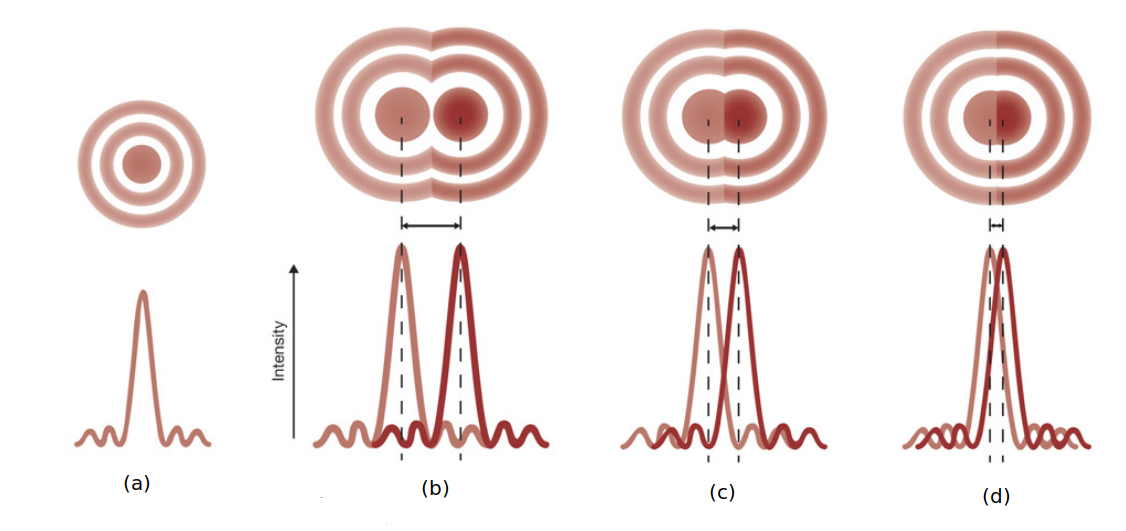
\includegraphics[scale=0.4]{images/airy_disks.png}
	\end{center}
	\centering
    \fadaptada{dunst2019imaging}
\end{figure}

As explained by \citeonline{goodman1996introduction}, an imaging system, particularly a set of microscope lenses, is said to be \emph{diffraction-limited} if the incident spherical light wave generated from a point-source object is transformed into another spherical wave which converges to an ideal image point, described by the original object point and affected by some sort of isotropic effect, such as magnification in a microscope.

The depth of field was described in \autoref{chapter:fundamentals-of-optics-and-light-microscopy} in terms of focal plane distances, but it may also be taken as the \emph{axial resolving power}, a measurement of resolution along the $z$ axis, determined by the numerical aperture and described by the Airy disk profile \cite{davidson2002optical}. Similarly to the Rayleigh's equation, the depth of field increases
with higher numerical apertures for the objective and shorter wavelengths of the incident light, and it represents a key property concerning the amount of blur in the resulting image.


\subsection{Point Spread Function and Image Formation Model}

\label{sec:point_spread_function_and_image_formation_model}

When light waves from a point source reach lenses, they suffer diffraction and refraction, which construct a new propagating set of rays that converge to a point in the center of the image plane in the shape of Airy disks; such shape is called the \sigla{PSF}{Point Spread Function}
of the imaging system (also called \emph{impulse response}), and it is intrinsically related to the imaging process \cite{wu2008microscope}. Particularly, the bright-field microscopy employs polychromatic nonpolarized incoherent light. From this concept, it is possible to relate the Airy disks to the PSF, since those are intensity distributions for each point source of light emanating from the specimen. \autoref{fig:point_spread_function}.(a) presents a theoretical scheme of imaging for a point source of light, and \autoref{fig:point_spread_function}.(b) depicts the shape of a incoherent PSF:

\begin{figure}[htb]
	\centering
	\caption{\label{fig:point_spread_function} Point Spread Function generated by a focused diffraction-limited system with incoherent light.} 
	\begin{center}
	    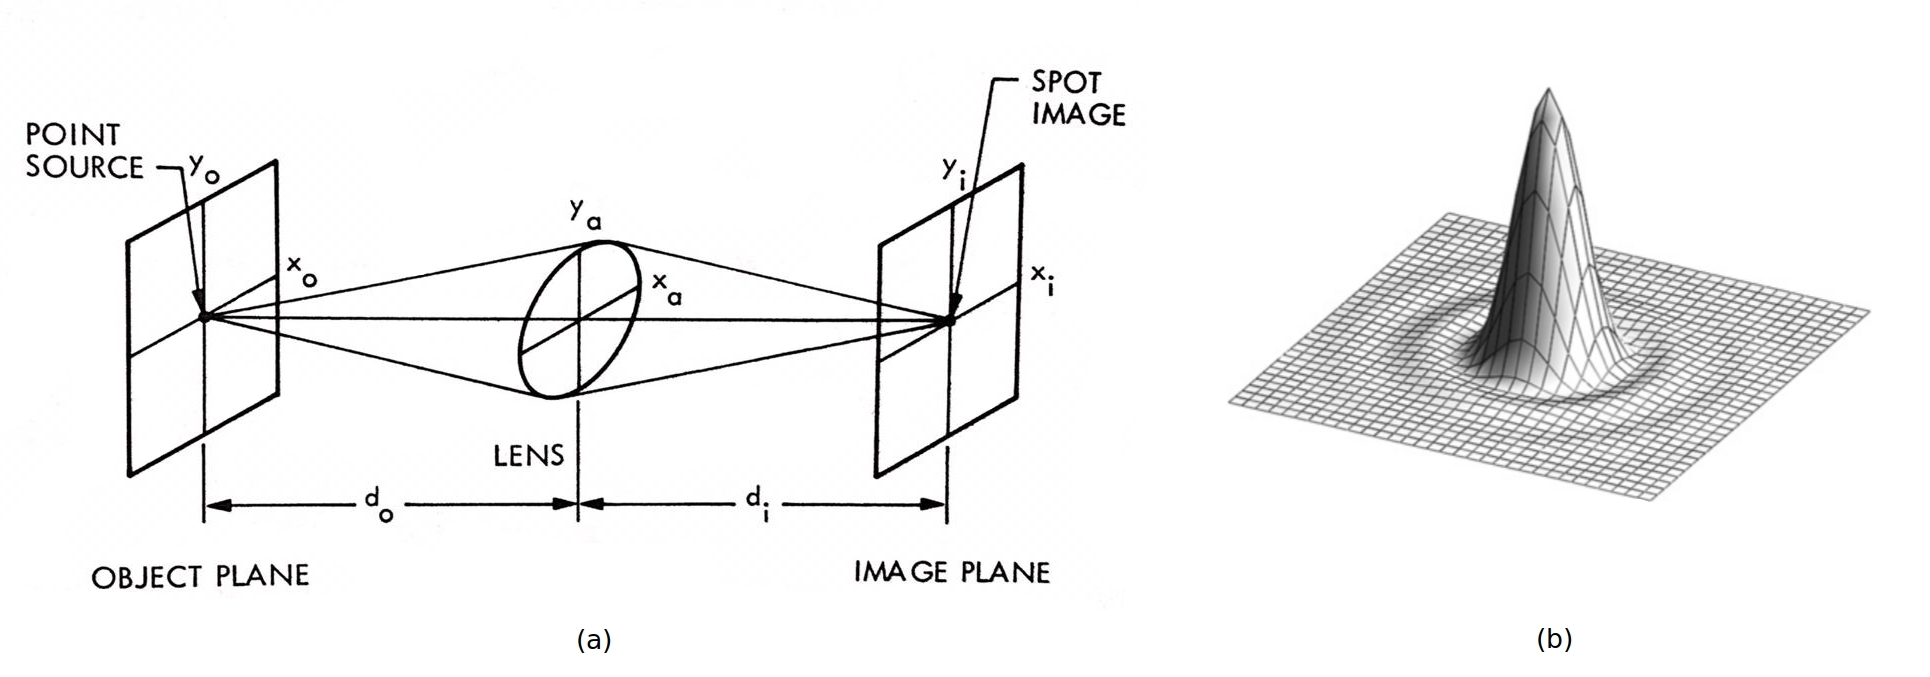
\includegraphics[scale=0.235]{images/point_spread_function.jpeg}
	\end{center}
	\centering
    \fadaptada{castleman1996digital,wu2008microscope}
\end{figure}

In \autoref{fig:point_spread_function}.(a), the imaging system in in focus, which is given by

\begin{equation}
\label{eqn:lens_focus}
\frac{1}{d_{o}} + \frac{1}{d_{i}} = \frac{1}{f},
\end{equation}

\noindent where $f$ is the focal length of the lens, $d_{o}$ and $d_{i}$ are respectively the distances from the point source plane to the lens and the distance from the image plane to the lens; the intensity of light in the point source is directly proportional to the intensity in the image, what characterizes a \emph{two-dimensional linear system} \cite{castleman1996digital}. Still according to \citeonline{castleman1996digital}, any motion of the point source on its plane moves the image is dictated by the law

\begin{align}
\label{eqn:isoplanatic_motion}
x_{i} = -\frac{d_{i}}{d_{o}}x_{o}
&&
y_{i} = -\frac{d_{i}}{d_{o}}y_{o},
\end{align}

\noindent where $(x_{o},y_{o})$ are the coordinates for the object location on its plane and $(x_{i},y_{i})$ are coordinates that locate the image on its plane. This implies that the shape of the image will not change according to the object's location, and this property yield \emph{shift invariance} to the system, which may be called \emph{isoplanatic}. These properties are observed in an ideal imaging system - simple lenses are not isoplanatic and linear, and  consequently simple microscopes also. However, there are approximations and mathematical tools that allow advanced microscopes to be assumed isoplanatic and linear.

The PSF as related to the intensity distributions described by the Airy disks are limited to the area of the aperture. This means that the amount of light that reaches the image plane is truncated by the circular aperture, what is also true for the PSF. The truncation is mathematically represented by the \emph{pupil function}, which is zero outside the boundaries of the aperture and unity otherwise, and might include also information about wave aberrations of the lens \cite{goodman1996introduction}. As denoted by \citeonline{wu2008microscope} with some notation adjustments, the PSF of an incoherent illuminated circular aperture imaging system is the Fourier Transform (explained further in \autoref{chapter:theoretical-background}) of the generalized pupil function, given by

\begin{equation}
\label{eqn:incoherent_psf}
h_{\lambda}(x,y,z) = \int_{-\infty}^{\infty}
                     \int_{-\infty}^{\infty}
         P(u,v)
         e^{j 2 \pi z
            \left(
                \frac{u^{2} + v^{2}}{2 \lambda L^{2}}        
            \right)
        }
        e^{j 2 \pi
            \left(
                \frac{xu + yv}{\lambda L}        
            \right)
        }
        du dv,
\end{equation}

\noindent where $h_{\lambda}(x,y,z)$ is point spread function for a light with wavelength $\lambda$, $P(x,y)$ is the pupil function, $z$ is the axial location the focal plane and $L = r / NA$ is the focal length, i.e. ratio between the radius of the circular aperture of the objective and the numerical aperture. The normalized Fourier Transform of the PSF is called \sigla{OTF}{Optical Transfer Function} \cite{castleman1996digital}.

From this framework, the image is formed as a set of impulse responses from each point in the object plane that where magnified by the imaging system. Linear systems possess a general expression, a convolution (which will be explained in \autoref{chapter:theoretical-background}) of the input with the system's impulse response, that describes the output \cite{brigham1988fast}. In this sense, the resulting image is a convolution of the PSF with the original image, defined as

\begin{equation}
\label{eqn:image_formation_convolution}
g(x,y) = \int_{-\infty}^{\infty}
         \int_{-\infty}^{\infty}
         h(x-u, y-v)f(x,y)du dv,
\end{equation}

\noindent where $f(x,y)$ is the original image, $g(x,y)$ is the observed image, $h(x,y)$ is the PSF of the imaging system and $u,v$ are shift parameters.

\subsection{Discrete Image Formation Model}

Digital images follow a discrete model for image formation due to the acquisition process: the spherical waves that leave the objectives reach the surface of \sigla{CCD}{Charge-coupled Devices}, sensors which proportionally converts light intensities to electrical signals that digitized as pixels \cite{gonzalez2018digital}. The digital images are matrices of pixels that represent light intensities with different channel configurations, where the most common one is the \sigla{RGB}{Red, Green and Blue} image. Therefore, similarly to the image formation model shown in \autoref{sec:point_spread_function_and_image_formation_model}, the two-dimensional digital image formation is described with a discrete process, arbitrarily as

\begin{equation}
\label{eqn:discrete_image_formation}
g[x,y] = h[x,y] \ast f[x,y],
\end{equation}

\noindent where $\ast$ denotes the discrete convolution, $g$, $h$ and $f$ are respectively the observed image, the discrete PSF of the imaging system and the original image, and $x,y \in \mathbb{Z}$. The discrete PSF of an imaging system with incoherent illumination and a circular aperture is given by

\begin{align}
\label{eqn:discrete_psf}
h(r) = \left[
        2
        \frac{J_{1}[\pi (r / r_{0})]}{\pi (r / r_{0})}
       \right]^{2},
&&
r = \sqrt{x^{2} + y^{2}},
&&
r_{0} = \frac{\lambda d_{i}}{a},
\end{align}

\noindent where $h(r)$ is the radially symmetrical PSF, $r$ is the radial distance, $r_{0}$ is a scaling factor, $J_{1}$ is the Bessel function of first order and first kind, $\lambda$ is the wavelength of the illumination, $a$ is the diameter of the aperture and $d_{i}$ is the distance from the lens plane to the image plane. A scheme of the geometric setup of discrete image formation through the PSF is shown in \autoref{eqn:discrete_image_formation}: 

\begin{figure}[htb]
	\centering
	\caption{\label{fig:discrete_psf_scheme} Geometric scheme of a lens' circular aperture and arbitrary point spread function profile.} 
	\begin{center}
	    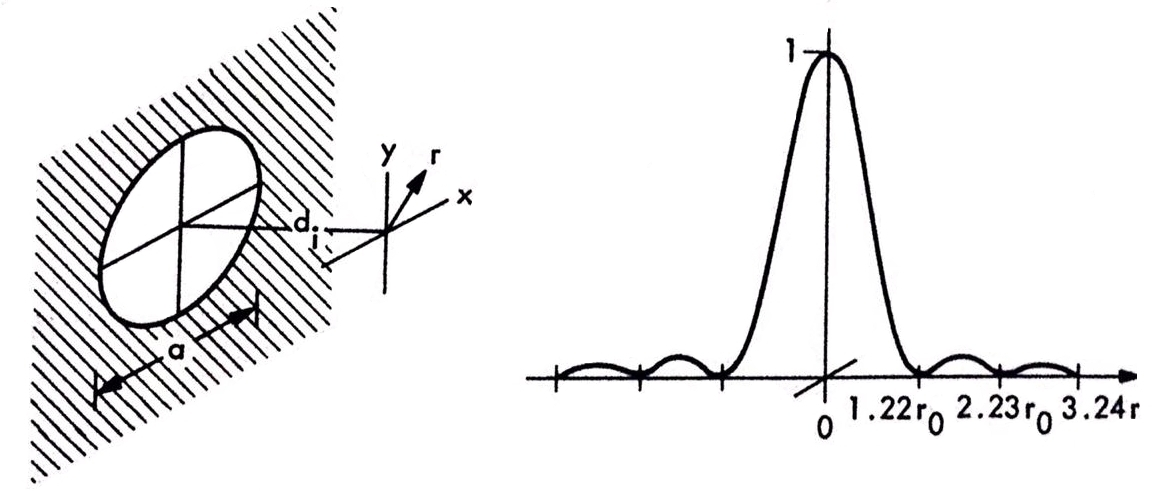
\includegraphics[scale=0.35]{images/discrete_psf_scheme.jpeg}
	\end{center}
	\centering
    \fadaptada{castleman1996digital}
\end{figure}

The discrete OTF is then the \sigla{DFT}{Discrete Fourier Transform} (explained in \autoref{chapter:theoretical-background}) of the PSF in \autoref{eqn:discrete_psf}. The OTF characterizes the intensities of light that emanate from the specimen in terms of frequencies. 

There is another property of image formation and acquisition that influences the image quality: the noise. Pursuant to \citeonline{wu2008microscope}, imaging is corrupted by intrinsic or extrinsic noise; the former is modelled by a Poisson distribution that influences each photon that reaches the sensor, and the latter is modelled by a Gaussian distribution that sums to the matrix of pixels. Details about noise are out of the scope of this work, since the degradation to be deeply explored is the defocus blur.

\section{Blur Characterization}
The \emph{blur} effect is one type of degradation that consists of global or local information loss in the image. There are three basic types of blur, generated by different processes: \emph{defocus blur}, \emph{motion blur} and \emph{Gaussian blur}. As explained in \autoref{sec:point_spread_function_and_image_formation_model}, the image formation process is subject to some constraints that limit its quality, such as the presence of noise or the convolution of the formed image with a point spread function. Such convolution results in defocus blur. 

The defocus blur is caused by the incidence of light within an aperture with significant dimensions, where the source of light is not properly placed in accordance to the focal plane; it is related to the variables of the optical system such as depth of focus, aperture, depth of field, aberrations and so on \cite{joshi2014defocus}. According to \citeonline{smith2007modern}, every optical system exhibits blur properties, in higher or lower proportions, due to the depth of focus and its adjustment. Therefore, blurring is unavoidable to a certain extent, hence every imaging device possesses a PSF due to its optics. The PSF is also named \emph{blur kernel}.

The motion blur occurs due to the relative motion between the camera and the scene, e.g. living cells in microscopy, during the acquisition; even though it is considered to be a degradation process, it may be used for aesthetic purposes, such as emphasizing the dynamic nature of a scene, obtaining motion information about the object or creating realistic images which are pleasing to the eye \cite{nayar2004motion}. Motion blur is usually an undesirable effect when it comes to fields such as microscopy, remote sensing or medical imaging, since it compromises analyses, pattern recognition tasks, predictions and several other applications.

The Gaussian blur is a general model of degradation and employs a particular kernel in order to smooth images. A convolution with such kernel promotes a Gaussian average among each region, and is usually employed in photography for styling effects or in edge detection (this application will be explained further in this work). Its kernel \cite{nixon2019feature} is given by

\begin{equation}
\label{eqn:gaussian_blur}
k(x,y) = e^{-
            \left( 
                \frac{x^{2} + y^{2}}{2 \sigma^{2}}
            \right)
            },
\end{equation}

\noindent where $\sigma^{2}$ is the variance of the Gaussian function. \autoref{fig:defocus_motion_blur} shows an example of large scale defocus and motion blur.

\begin{figure}[H]
	\centering
	\caption{\label{fig:defocus_motion_blur}Defocus blur (left) and motion blur (right) in large scales.}
	\begin{center}
	    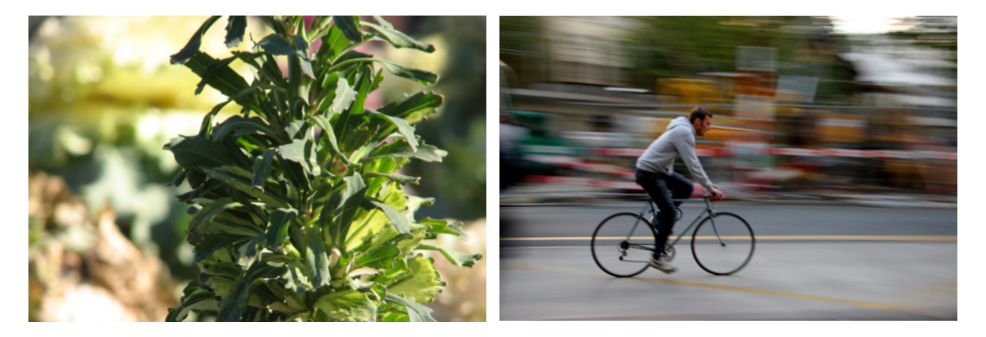
\includegraphics[scale=0.4]{images/fig7.png}
	\end{center}
	\centering
    \fadaptada{su2011blurred}
\end{figure}

Finally, another useful way to mathematically describe the point spread function is through the Dirac Delta. It consists of a generalized function that represents an impulse, i.e. an infinitely high value within an infinitely small period of time \cite{bracewell2000fourier}. \autoref{fig:psf} shows an arbitrary example of a punctual source of light and its image, which suffers the spreading effect.

\begin{figure}[H]
	\centering
	\caption{\label{fig:psf} Magnified image of a light impulse (left) and its impulse response function, the PSF (right).}
	\begin{center}
	    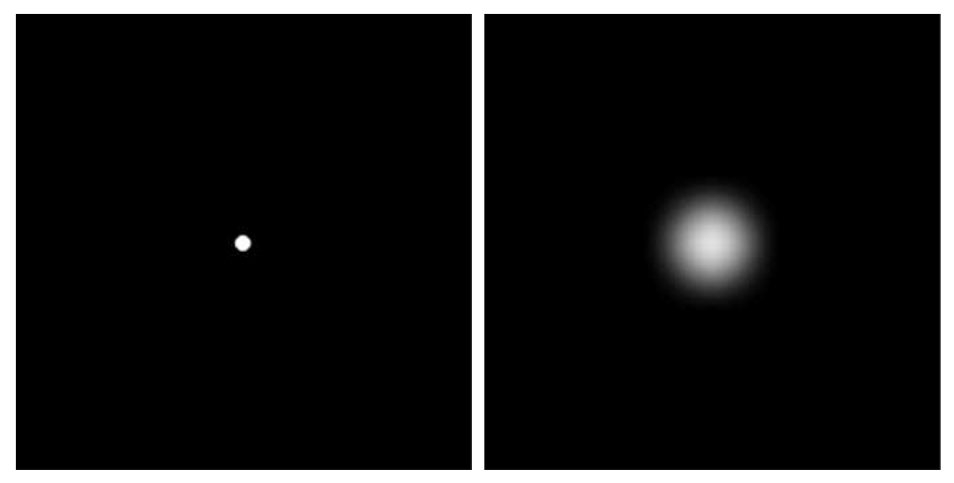
\includegraphics[scale=0.4]{images/fig8.png}
	\end{center}
	\centering
    \fadaptada{gonzalez2008digital}
\end{figure}

Namely, it is a function $\delta(x)$ that is zero-valued for any $x \neq 0$ and is infinity-valued for $x = 0$. This property can be combined with any smooth function $f\colon \mathbb{R}^{n} \to \mathbb{R}^{n}$.
The continuous Dirac Delta may be written, as stated by \citeonline{weisstein2020delta}, as

\begin{align}
\label{eqn:dirac_delta_function}
\delta^{2}(x,y)= 
\begin{cases}
    \infty, & \text{if } x^{2} + y^{2} =0\\
    0, & \text{if } x^{2} + y^{2} \neq 0
\end{cases},
&&
\int_{-\infty}^{\infty}
\int_{-\infty}^{\infty}
\delta^{2}(x,y)dxdy = 1.
\end{align}

\noindent The discrete version of the Dirac Delta function consists of an infinite sum instead of the integral. This concept of impulse is the point source of light, concerning images. It provides the blurring effect on images, as it promotes the diffusion of the acquired information.


% \chapter{Theoretical Background}
% \label{chapter:theoretical-background}
% \simbolo{\ast}{Convolution}

This chapter summarizes the relevant theoretical concepts, methods, and tools for the development of our approach to select partially sharp images among a z-stack dataset and merge the best information from each selected image into a high-quality image. The mathematical and image processing concepts needed to develop our method are convolutions, transforms, enhancement, registration, fusion and quality assessment; statistical methods are used as a bridge between yielding a quantitative index of image quality and merging pixels, as well as evaluating the performance.

\section{Convolution and Image Transforms}
As seen in Chapters \ref{chapter:fundamentals-of-optics-and-light-microscopy} and \ref{chapter:blur-characterization-and-image-formation}, the processes of image formation and acquisition concerning linear systems are subject to some operations, i.e. the convolution, the \sigla{FT}{Fourier Transform} and its continuous and discrete versions, that modify the original representation of the scene. The linear system theory provides mathematical tools to explore those operations and others, such as sampling, filtering, and enhancement; it describes the behavior of electrical circuits and optical systems \cite{castleman1996digital}.

According to \citeonline{bracewell2000fourier}, the convolution of two arbitrary functions $s$ and $t$ results in another function $r$ is, with notation adjustments, defined by the integral

\begin{equation}
\label{eqn:one_dimensional_convolution}
r(x) = \int_{-\infty}^{\infty}s(u) t(x - u) du,
\end{equation}

\noindent where $x$ is the one-dimensional coordinate and $u$ is a shifting parameter. In other words, this procedure is compared to moving a 180 degrees-rotated filter mask over the function values and computing the sum of products at each location \cite{gonzalez2018digital}. Hence, the shifting parameter represents the slide of the filter mask above the values. As seen in Chapter~\ref{chapter:blur-characterization-and-image-formation}, convolution is responsible for the image formation and acquisition processes, but it also covers several other applications, e.g. smoothing, sharpening and reducing noise in images. Similarly to the one-dimensional case and pursuant to \citeonline{castleman1996digital}, the two-dimensional convolution is denoted by

\begin{equation}
\label{eqn:two_dimensional_convolution}
r(x,y) = \int_{-\infty}^{\infty}
         \int_{-\infty}^{\infty}
         s(u,v) t(x - u, y - v) du dv,
\end{equation}

\noindent where $u$ and $v$ are shifting parameters, $\ast$ denotes the convolution. The \emph{spatial domain} is the subset of the real plane where functions like $r$, $s$ and $t$ are spanned, and $(x,y)$ as points within such subset are named spatial variables; consequently, any mathematical operation that employs pixels from this subset are named spatial domain techniques. Concerning the digital image processing applications, which deals with images as matrices of pixels, the discrete two-dimensional convolution for an image $f(x,y)$ and a function $h(x,y)$ is given by 

\begin{equation}
\label{eqn:2d_discrete_convolution}
g(x,y) = h(x,y) \ast f(x,y) = 
        \sum_{m=-a}^{a}
        \sum_{n=-b}^{b}
        f(m,n) h(x-m,y-n),
\end{equation}

\noindent where $a = (m-1)/2$ and $b = (n-1)/2$, given that the function $h(x,y)$ is considered to be a two-dimensional filter of size $m \times n$ \cite{gonzalez2018digital}.

Convolution, together with several other operations employed in this work, operate directly on the spatial domain by modifying pixel values based on mathematical constraints. Some of those operations may have issues that hinder the operation, e.g. the computation time of a convolution process should be finite, otherwise, its use is impractical; this is one of the reasons why \emph{image transforms} are widely used. They encompass any group of mathematical operations that transfers the input signal or image from its domain to the transform domain \cite{gonzalez2008digital}. Let $s$ be an arbitrary two-variable function, $t_{f}$ and $t_{i}$ be the forward and inverse transformation kernels, respectively. The general discrete form of the forward and inverse two-dimensional transforms is denoted by 

\begin{align}
\label{eqn:generic_transform}
R(u,v) = 
\sum_{x=0}^{M-1}
\sum_{y=0}^{N-1}s(x,y)t_{f}(x,y,u,v)
&&
s(x,y) = 
\sum_{x=0}^{M-1}
\sum_{y=0}^{N-1}R(u,v)t_{i}(x,y,u,v),
\end{align}

\noindent where $M$ and $N$ are the dimensions of the image, $x$ and $y$ are coordinates of the image, $u = \{0,1,2,...,M-1\}$ and $v = \{0,1,2,...,N-1\}$ are called transform variables. The $t_{f}$ function is responsible for the forward domain change and the $t_{i}$ transfers the image back to the spatial domain. The domain switch allows different approaches to operations to be executed and present features of the image that could not be represented in the spatial domain. The convolution operation, for instance, turns itself into a simple matrix multiplication task on the Fourier Transform domain (which will be detailed in the following sections) and that solves the performance constraint.

\section{Continuous and Discrete Fourier Transform}
Regarding image transforms, one of the most important examples is the Fourier Transform. It was conceived by Jean Baptiste Joseph Fourier (1768 - 1830) and states that any periodic function can be expressed as the sum of sines and cosines of different frequencies, each multiplied by a different coefficient \cite{gonzalez2018digital}. According to \citeonline{brigham1988fast}, the relationship between the different frequency sinusoids and arbitrary function $s$ to be analyzed is described as

\begin{equation}
\label{eqn:fourier_transform}
S(f) = \int_{-\infty}^{\infty}s(x)e^{-j 2 \pi f x} dx,
\end{equation}

\noindent where $S(f)$ is the Fourier Transform of the $s(t)$ and $j = \sqrt{-1}$ represents the imaginary unit. Note that the function transformed from the one-dimensional spatial domain to the frequency domain, represented by $f$. Similarly, the inverse transform is denoted by

\begin{equation}
\label{eqn:inverse_fourier_transform}
s(x) = \int_{-\infty}^{\infty}S(f)e^{j 2 \pi f x} df.
\end{equation}

As stated by \citeonline{bracewell2000fourier}, an arbitrary periodic function $s$ with period $T$ is commonly to express it as a Fourier series, given by the expression

\begin{equation}
\label{eqn:fourier_series}
a_{0} + \sum_{1}^{\infty} (a_{n} \cos{2 \pi n f t} + b_{n} \sin{2 \pi n f t}),
\end{equation}

\noindent where

\begin{align*}
a_{0} &= \frac{1}{T} \int_{-\frac{1}{2} T}^{\frac{1}{2} T} s(t) dt\\
a_{n} &= \frac{2}{T} \int_{-\frac{1}{2} T}^{\frac{1}{2} T} s(t) \cos{(2 \pi n f t)} dt\\
b_{n} &= \frac{2}{T} \int_{-\frac{1}{2} T}^{\frac{1}{2} T} s(t) \sin{(2 \pi n f t)} dt.\\
\end{align*}

If the function is not periodic, then the Fourier Transform is applied as a continuous function of frequency, i.e. $s(t)$ is represented by the sum of sinusoids of all frequencies \cite{brigham1988fast}. Particularly, this stands for images, which are non-periodic functions. The common approach is to appraise the image as a section of a periodic function so the use of Fourier Transform makes sense.

The Equations \ref{eqn:fourier_transform} and \ref{eqn:inverse_fourier_transform} together are named a \emph{Fourier Transform pair}. Images are represented by two-variable functions, which motivates the use of a two-dimensional Fourier Transform; moreover, as digital images are matrix representations of images, the two-dimensional Discrete Fourier Transform is the most relevant brand of the FT for image processing applications. Consequently, the two-dimensional Fourier Transform pair of a function $s(x,y)$ is given by

\begin{align}
\label{eqn:two_dimensional_continuous_fourier_transform}
S(u,v) &= \int_{-\infty}^{\infty}
         \int_{-\infty}^{\infty}
         s(x,y) e^{-j 2 \pi 
                    \left(
                        ux + vy
                    \right)
                  }
        dx dy\\
s(x,y) &= \int_{-\infty}^{\infty}
         \int_{-\infty}^{\infty}
         S(u,v) e^{j 2 \pi 
                    \left(
                        ux + vy
                    \right)
                  }
        du dv.
\end{align}

According to \citeonline{bracewell2000fourier}, this pair of equations represents the analysis of $s(x,y)$ into components of the form $\exp{\left[j 2 \pi (ux + vy) \right]}$, where the variables $u$ and $v$ represent spatial frequencies. The equation that relates such components to sinusoids is the \emph{Euler's Formula} or \emph{Euler's Identity}, written as

\begin{equation}
\label{eqn:euler_formula}
    e^{j\theta} = \cos{\theta} + j\sin{\theta}
\end{equation}

\noindent where $\theta = 2 \pi f$ is a number that represents an angle in radians and $e^{j\theta}$ is the polar form representation of the sinusoids \cite{gonzalez2018digital}. Finally, the common two-dimensional DFT form applied among image processing is, as reported by \citeonline{gonzalez2018digital}, denoted by

\begin{align}
\label{eqn:two_dimensional_discrete_fourier_transform}
S(u,v) &= \sum_{x = 1}^{M}
          \sum_{y = 1}^{N}
          s(x,y) e^{-j 2 \pi 
                    \left(
                        ux/M + vy/
                    \right)
                  }
        dx dy\\
s(x,y) &= \frac{1}{MN}
          \sum_{1}^{M}
          \sum_{1}^{N}
          S(u,v) e^{j 2 \pi 
                    \left(
                        ux/M + vy/N
                    \right)
                  }
        du dv,
\end{align}

\noindent where $s(x,y)$ is a discrete function that represents an image of size $M \times N$, $x$ and $y$, discrete variables that represent spatial coordinates, $u$ and $v$ are discrete spatial frequencies. 

One prominent example of Fourier Transform use is the Convolution Theorem. It states that convolution may be computed by a multiplication in the Fourier domain \cite{brigham1988fast}. This allows much faster computations of convolution in comparison to the spatial domain approach and is frequently used in many applications, such as image filtering and convolutional neural networks. In terms of computational complexity, the common two-dimensional Discrete Fourier Transform implementations yield results in $\mathcal{O}(n^{2})$ time for square or zero-padded images and $\mathcal{O}(mn)$ for images of size $m \times n$; for this reason, the \sigla{FFT}{Fast Fourier Transform} is a divide-and-conquer implementation created by Cooley and Tookey in 1965 and reduces the computational complexity to $\mathcal{O}(n \log n)$ \cite{bracewell2000fourier}. The Fourier Transform is widely employed in this work and the chosen approach to compute it is the FFT algorithm.

\section{Image Enhancement}
With a clear panorama of convolution and Fourier transform concepts, it is possible to enlighten the \emph{image enhancement} concept and its relevant applications to this work. Image enhancement is the process of manipulating an image in order to provide a resulting representation that is more suitable for a particular problem, e.g. an enhancement method for medical images may not be efficient for satellite images \cite{gonzalez2018digital}. Within microscopy, image enhancement is desirable due to the limited capacity of optical imaging devices and also the features of each microscopy technique, e.g. acquisition with different illumination settings, focal planes, time intervals or spectral channels; hence, enhancement algorithms for microscopy should cover all types of information \cite{wu2008microscope}. According to \citeonline{wu2008microscope}, image enhancement techniques are divided into \emph{spatial domain}, \emph{Fourier transform} and \emph{wavelet transform} methods and will be described as follows. 

The spatial domain methods are basically transforms that globally maps the gray levels of an image (or the gray levels the channels from a multichannel image, such as RGB) to their enhanced stated. Some examples are contrast stretching, which adjusts all gray levels of an image to fit among the desired range, thresholding, which applies a decision function that creates a binary image based on a preset gray level, histogram equalization, and spatial filtering. Particularly, histogram equalization and spatial filtering play an important role in this work and therefore will be explored further.

Fourier transform domain methods operate with images as a distribution of frequencies since some features are better described by it. Noise, for example, may be suppressed in a sharpening process or reduced by amplifying mid-frequency components and attenuating high-frequency ones. The Wiener Filtering process is an extensively used example of a frequency domain enhancement method that recovers a noisy signal or image based on estimations of spectral properties from the original image. Other examples of Fourier domain enhancement are band-pass filters and least-squares deconvolution applications.

Finally, the wavelet transform based methods enhance images based on Wavelet Transforms, i.e. mathematical frameworks that decompose signals and images into frequency components in different scales. Some approaches such as thresholding may be applied to wavelet coefficients, and since the output of wavelet transforms depend on the chosen wavelet function, many possible variants depend on the image features. 

\subsection{Histogram Equalization}

The image histogram is one of the simplest and most useful tools in image processing and consists of a function that summarizes the gray level content of an image in terms of a frequency distribution \cite{castleman1996digital}. The histogram equalization consists of applying a non-linear monotonic mapping to provide an approximation of a uniform distribution to the output image's histogram \cite{gonzalez2018digital}. The output histogram is a normalization of the cumulative histogram of the image, given by

\begin{equation}
\label{eqn:histogram_equalization}
hist_{equalized}(r) = \frac{L - 1}{MN} hist_{cumulative}(r),
\end{equation}

\noindent where $hist_{equalized}(r)$ and $hist_{cumulative}(r)$ are the equalized and cumulative histograms relative to a range $L$ of intensities after image quantization with $r$ values, $M \times N$ is the image resolution. Since it stems from a sum of probabilities and no new gray intensity levels should be created, the process generates fractional values that are mapped onto integers. The result of this process is contrast enhancement, which may be seen in Figure \ref{fig:histogram_equalization}:

\begin{figure}[htb]
	\centering
	\caption{\label{fig:histogram_equalization} Example of histogram equalization of dark and light images of a scene.} 
	\begin{center}
	    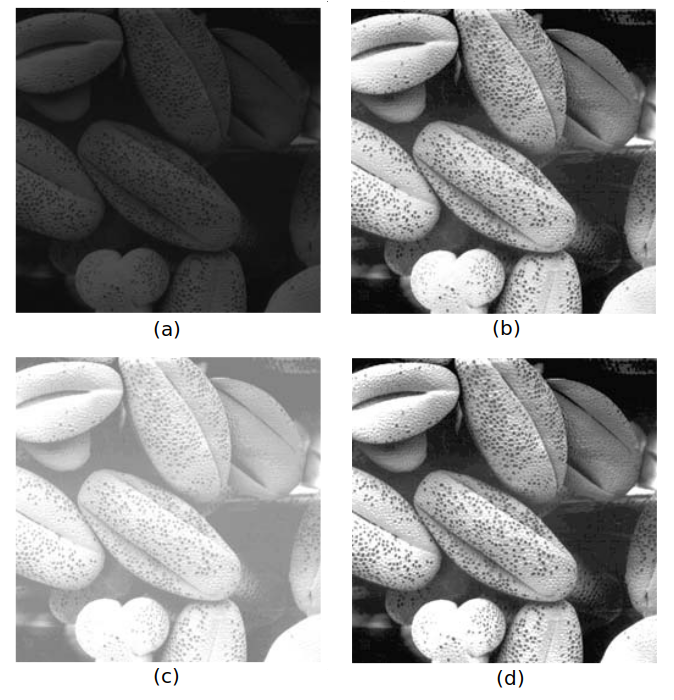
\includegraphics[scale=0.5]{images/histogram_equalization.png}
	\end{center}
	\centering
    \fadaptada{gonzalez2018digital}
\end{figure}

\subsection{Spatial Filtering}

Spatial filtering consists of the convolution of an image with a predefined kernel operator, which creates new pixel values and replaces them in the original image \cite{gonzalez2018digital}. The continuous form may be represented as a convolution over all values of a defined region of the image and the discrete form consists of sliding a weight mask over the image \cite{wu2008microscope}. Figure \ref{fig:generic_spatial_filtering} presents an arbitrary schema of a basic linear spatial filtering procedure:

\begin{figure}[htb]
	\centering
	\caption{\label{fig:generic_spatial_filtering} Arbitrary example of linear spatial filtering of an image (a) with a $3 \times 3$ filter mask (b), which results in filtered sections (c).} 
	\begin{center}
	    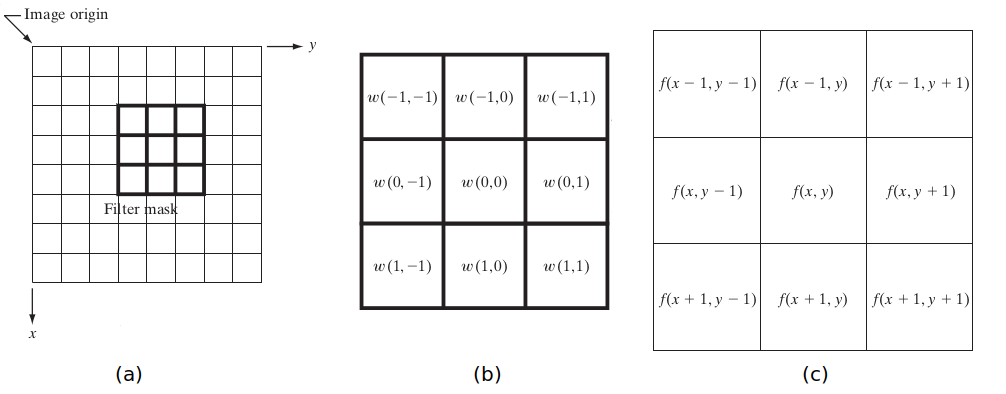
\includegraphics[scale=0.4]{images/generic_spatial_filtering.png}
	\end{center}
	\centering
    \fadaptada{gonzalez2018digital}
\end{figure}

Examples of discrete spatial filtering in digital image processing are smoothing filters, order-statistic nonlinear filters and sharpening filters, illustrated according to \cite{gonzalez2018digital}. Smoothing spatial filters are applied to remove small details, edges and lines from an image, i.e. blur, or to reduce noise. The order-statistic nonlinear filters are based on ordering pixels of the image under the filter area and replacing the pixel value in the center of the area with the response from ordering; one example is the \emph{median filter}, which replaces the center pixel with the median of pixels in its neighborhood. Median filters yield significant noise reduction effects if the nature of the noise is random. Finally, the sharpening filters are built to highlight transitions in intensity by spatial differentiation and are used for enhancing edges.

\subsection{Contrast Limited Adaptive Histogram Equalization}

Contrast enhancement may be described as the slope of the function that is relating input image intensity value to desired resultant image intensities \cite{sonali2019approach}. Histogram equalization is one of the techniques to perform contrast enhancement and works in an image by mapping the distribution of its gray levels to an approximately uniform distribution. The performance of this process is deeply related to the amount of noise in the image since it consists of peaks in the histogram, which unbalances the mapping and enhances noisy structures. One solution to this problem, according to \citeonline{zuiderveld1994constrast}, is to divide the image into \emph{contextual regions}, i.e. rectangular areas of $8 \times 8$ size, compute the optimal contrast for each of the regions and merge the results with bilinear interpolation to avoid boundary effects. This method is known as \sigla{AHE}{Adaptive Histogram Equalization}, where the global outlier gray levels do not influence each contextual region contrast enhancement.

The \sigla{CLAHE}{Contrast Limited Adaptive Histogram Equalization} method was proposed to overcome the drawback of noise. As stated by \citeonline{sonali2019approach}, it is the method that improves the low contrast issue and operates by limiting the contrast enhancement that is usually performed by ordinary histogram equalization or the AHE, which results in the noise enhancement as well. It is accomplished by allowing only a maximum number of pixels in each of the histogram bins and equally distributing the clipped pixels among the whole histogram \cite{zuiderveld1994constrast}. Figure \ref{fig:hr_ahe_clahe} presents an example of the differences between histogram equalization techniques and their results in a \sigla{MRI}{Magnetic Resonance Imaging} example:

\begin{figure}[htb]
	\caption{\label{fig:hr_ahe_clahe} MRI image of a human knee \textbf{(a)}, a simple histogram equalization \textbf{(b)}, an adaptive histogram equalization \textbf{(c)} and the contrast limited adaptive histogram equalization \textbf{(d)}.} 
	\begin{center}
	    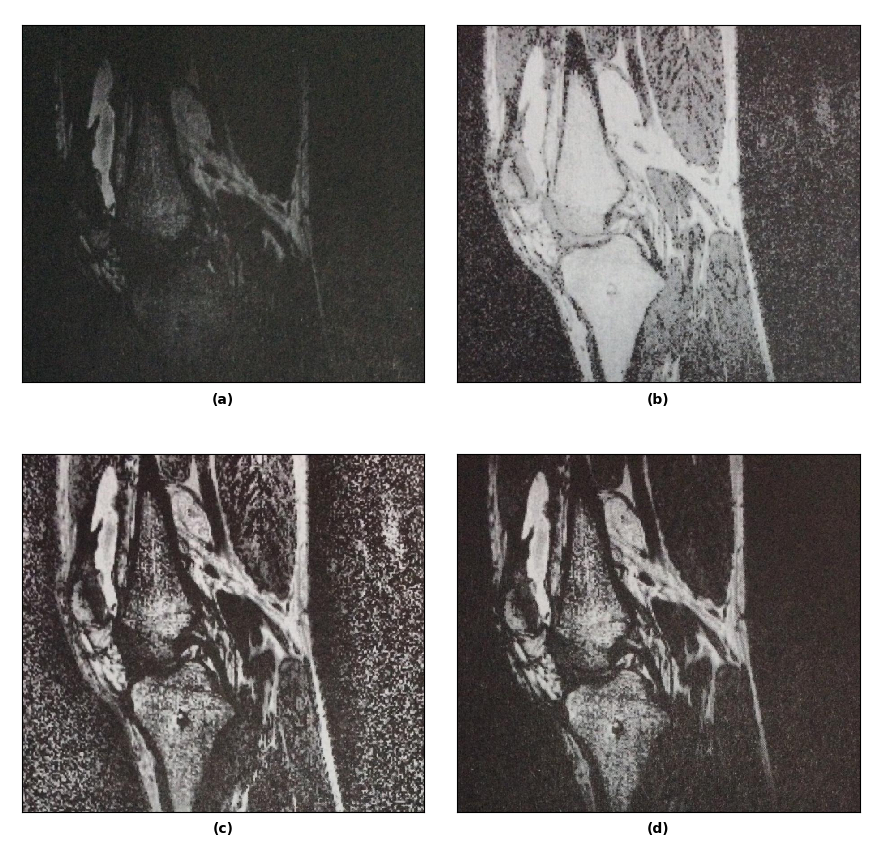
\includegraphics[scale=0.4]{images/knee_HE_AHE_CLAHE.png}
	\end{center}
	\centering
    \fadaptada{zuiderveld1994constrast}
\end{figure}


\section{Image Registration}
When a set of images of the same scene is acquired in different conditions such as distinct focus configurations, sensors or times, each image should be geometrically aligned according to a reference image if the final imaging application requires a combination of each image content. The process of overlaying two or more images with different acquisition settings is named image registration and plays an important role as a pre-processing step for image fusion, change detection and multichannel image restoration \cite{zitova2003image}. According to \citeonline{gonzalez2018digital}, magnetic resonance imaging and positron emission tomography systems, for example, are two different sensors that may acquire medical images that need to be registered; images which were taken in different times such as satellite images also need to be registered.

The image registration methods consist of the following steps, as reported by \citeonline{zitova2003image} and \citeonline{gonzalez2018digital}:

\begin{itemize}
    \item \emph{Feature detection}: the first step is to manually or automatically detect distinctive objects, e.g. edges, contours, corners and represent those as \emph{control points}, i.e. points with known locations in the reference and input images;

    \item \emph{Feature matching}: a relationship between the detected features in each image is established using feature descriptors;

    \item \emph{Transform model estimation}: this step consists of estimating parameters for mapping functions that align the input images with the reference image, either by establishing feature correspondence or performing an optimization procedure;

    \item \emph{Image resampling and transformation}: finally, the transformation occurs and the image is resampled with interpolation techniques.

\end{itemize}

Practically, the image registration is a mapping between two or more images by means of a spatial transformation and an intensity transformation \cite{brown1992survey}. Some prominent examples of registration methods are the principal axes, multiresolution, optimization-based, boundary, model-based and adaptive methods  \cite{goshtasby2012image}. The spatial transformations play an important role in all image registration techniques, and the most common general examples are rigid, affine, projective, perspective and global polynomial \cite{brown1992survey}. Still pursuant to \citeonline{brown1992survey}, each of such transformations may be described as:

\begin{itemize}
    \item \emph{Rigid}: This type of transformation accounts for object or sensor movement in which objects in the images retain their relative shape and size, and a \emph{rigid-body transformation} is an example, composed of a combination of rotation, translation, and scale change; 
    
    \item \emph{Affine}: Those are capable of tolerating more complicated distortions and preserve mathematical properties, and the \emph{shear transformation} is an example;
    
    \item \emph{Projective and Perspective}: The former deals with distortions due to projection of the objects at varying distances to the sensor onto the image plane, and the latter demands prior knowledge about the locations of the objects in the scene relative to the sensor;
    
    \item \emph{Polynomial}: Finally, the polynomial transformations can cover the broadest range of distortions, as long as those are approximately homogeneous among the image.
\end{itemize}

In the scope of this work, the microscopy images were registered with a particular combination of methods. The feature extraction was done with a custom implementation of the \sigla{SIFT}{Scale Invariant Feature Transform}, together with a custom extension of the \sigla{RANSAC}{Random Sample Consensus} method for parameter estimation and the geometric consensus filtering process with the expected transformation model and a maximal expected error as parameters \cite{saalfeld2019computational}. Those techniques will be described next.

\subsection{Scale-invariant feature transform}

As originally proposed by \citeonline{lowe1999object}, the SIFT is a feature extraction approach for object and scene recognition which consists of the following steps:

\begin{itemize}
	\item \emph{Scale-space extrema detection}: Initially, a difference-of-Gaussian function is applied in order to identify the invariant scale and orientation keypoints;
    
    \item \emph{Keypoint localization}: Each keypoint candidate is selected based on measures of their stability;
    
    \item \emph{Orientation assignment}: One ore more orientations are assigned to each keypoint location based on image gradient directions;
    
    \item \emph{Keypoint descriptor}: Finally, a measurement of the local image gradients is done for the particular scales and neighborhood of each keypoint, followed by a    transformation of those into a proper representation.
	
\end{itemize}

The custom SIFT implementation is described here as proposed by \citeonline{lowe2004distinctive}. The difference-of-Gaussian method for the detection of scale-space extrema is a convolution of an image $f(x,y)$ with the difference of two nearby scales of distance $k$, given by

\begin{equation}
\label{eqn:DoG}
D(x,y,\sigma) = \left(G(x,y,k \sigma) - G(x,y,\sigma)\right) f(x,y),
\end{equation}

\noindent where $D(x,y,\sigma)$ is the result of the convolution and $G(x,y,\sigma)$ stands for a Gaussian function described as

\begin{equation}
\label{eqn:gaussian_function}
G(x,y,\sigma) = \frac{1}{\sqrt{2 \pi \sigma}} e^{- \frac{x^{2} + y^{2}}{\sigma^{2}}}.
\end{equation}

The difference-of-Gaussians is constructed by convolving the image with several Gaussians separated by the multiplicative factor $k$, followed by a division of the scale-space by means of multiplying $\sigma$ by two at each scale change. Later, the local maxima and minima (extrema) are detected by checking around 8-neighborhoods in the current image and 9-neighborhoods within the image in adjacent scales.

With the scale-space extrema in hands, the keypoints are localized by fitting a 3D quadratic function of local sample points with the Taylor expansion

\begin{equation}
\label{eqn:taylor_DoG}
D(\mathbf{x}) = D + 
                \frac{\partial D^{T}}{\partial  \mathbf{x}}\mathbf{x} + \frac{1}{2}\mathbf{x^{T}}\frac{\partial^{2} D}{\partial \mathbf{x}^{2}}\mathbf{x},
\end{equation}

\noindent where the derivatives of the difference-of-Gaussians matrix $D$ is computed at the sample point and $\mathbf{x} = (x,y,\sigma)^{T}$ is the offset for such point. The extremum location is found with the derivative of $D$ with respect to $\mathbf{x}$ and setting it to zero. The value of $D$ at the extremum provides a way to include only stable and good contrast extrema. Together with this low contrast keypoint exclusion, it is necessary to exclude those which possess a large principal curvature across the edge direction and a small one in its perpedicular direction; this is achieved by means of a threshold based on the sum and product of the eigenvalues from the trace and determinant of a Hessian matrix computed at the location and scale of each keypoint.

The next step is to provide the orientation of each keypoint concerning local image properties. This yields invariance to image rotation and is done by computing the gradient magnitude and the orientation for each smoothed image sample, denoted by

\begin{equation}
m(x,y) = \sqrt{(L(x + 1, y) - L(x - 1, y))^{2} + (L(x, y + 1) - L(x, y - 1))^{2}}
\end{equation}

\begin{equation}
\theta(x,y) = \tan^{-1}
			\left(
			\frac{L(x, y + 1) - L(x, y - 1)}
				 {L(x + 1, y) - L(x - 1, y)}
			\right),
\end{equation}

\noindent where $m(x,y)$ is the gradient magnitude, $\theta(x,y)$ is the orientation and $L(x,y)$ is the smoothed image, i.e. the observed image convolved with a Gaussian kernel. The obtained information is sampled around each keypoint location at the selected scale and Gaussian blur level, in order to generate the descriptor representation. The samples are then weighted by a Gaussian window and accumulated into orientation histograms that represent $4 \times 4$ subregions. The descriptors are computed from a $16 \times 16$ subarray. Finally, the advantages of the custom implementation of SIFT are the invariance to image rotation and scale, robustness across a substantial range of distortions (affine, additive noise and illumination changes) and computational efficiency.

The RANSAC algorithm is a non-deterministic iterative method of fitting a mathematical model to experimental data and also an outlier detector. \cite{fischler1981random}. Concerning the image registration application in this work, it is used to identify corresponding landmark points in overlapping image tiles \cite{saalfeld2019computational}. Then, the recognized matching points in each image undergo the geometric consistency filtering process with the expected transformation model and the maximal expected error parameters; this last filtering process aims to verify if all points support the same transformation model and yield the best matches concerning all points for each image of the dataset.

\section{Image Fusion}
Image fusion is a process that merges several images, possibly acquired in diverse conditions or with different cameras, into one image with higher quality, more details and consequently more useful for humans and computer tasks \cite{mitchell2010image}. Examples of image fusion applications are noise reduction, edge enhancement, and super-resolution. One traditional use of image fusion occurs in medical imaging fields; the quality of information about illnesses, cells, clinical analysis and several other medical tasks (including the computer-assisted ones) have found profitable results from the image fusion techniques and led themselves to better and faster decisions when it comes to human beings \cite{james2014medical}. There are also relevant applications in remote sensing multispectral images, segmentation of regions in different color spaces, biometry: the pan-sharpening process is the generation of a high-resolution multispectral image from low to high-resolution ones, K-Means segmentation and fusion of pixels in the RGB and the Iris Recognition biometric process with video frames are examples of such tasks, respectively \cite{mitchell2010image}.


Also according to \citeonline{mitchell2010image}, the general framework for the image fusion procedure consists of four stages: \emph{Multiple Input Images}, \emph{Common Representational Format}, \emph{Fusion} and \emph{Display}.
The multiple input images stage is simply the acquisition of the images to be merged. There are several approaches to this: the dataset may be captured from different sensors, under distinct light conditions or angles, with different magnifications, under several focus settings, and with temporal measurements, if the scene changes through time.

If the acquired dataset images do not share the same features such as dimension, rotation angle, and resolution, then the images should be pre-processed in order to arrive at a common state. This configures the common representational format step, which generates a new and temporary dataset with the same properties, e.g. color space, dimensions, and noise level. The fusion stage employs a decision method to dictate which regions, objects, colors or details will compose the final image; some methods rely on the wavelet transform, for example. Finally, the display stage provides a view of the resulting image, which can be used directly for any further task or even be the input for other image processing operations. \autoref{fig:fusion_general_framework} depicts an arbitrary example of the four stages. 

\begin{figure}[ht]
	\centering
	\caption{\label{fig:fusion_general_framework}Image fusion general framework. (a) Multiple Input Images, (b) Common Representational Format, (c) Fusion and (d) Display.}
	\begin{center}
    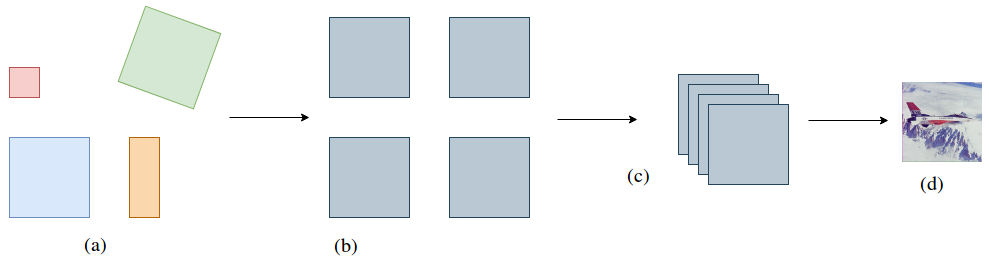
\includegraphics[scale=0.45, trim={0 -1.5cm 0cm -1.5cm}, clip]{images/image_fusion_scheme.png}
	\end{center}
	\centering
    \fautor
\end{figure}

The four arbitrary images in \autoref{fig:fusion_general_framework}.\textbf{(a)} represent different images of the same scene, taken at different resolutions, rotation angles, and shapes. In \autoref{fig:fusion_general_framework}.\textbf{(b)}, the images are all reshaped, converted to common color space and ready to undergo the processing algorithm which will transform them into feature vectors. \autoref{fig:fusion_general_framework}.\textbf{(c)} represents the image fusion by means of an arbitrary fusion rule. The resulting image is depicted in \autoref{fig:fusion_general_framework}.\textbf{(d)}. Since image fusion is only one branch of data fusion field, this procedure has a wide variety of approaches and methods; hence, the domain will be restricted to the multi-focus image fusion and some relevant related work will be presented in \autoref{chapter:related-work}.

\section{Image Quality Assessment}
\sigla{IQA}{Image Quality Assessment} is the evaluation of image quality as perceived by an average human observer, i.e. how close an image is to a given original or reference image. It is also related to the accuracy of the image acquisition process for an imaging system \cite{bovik2009essential}. It is known that images are frequently used in health and life sciences, public security systems, remote sensing, and several other fields; hence, there are computational applications that offer some useful service employing image processing. As a result, assessing image quality poses as an important task among those applications for which several techniques are being developed, evolved and deployed.

According to \citeonline{tang2019feature}, the IQA methods are distributed between the subjective assessment and objective assessment categories. The former is based on a well-defined test environment for random observers to label images and provide the final \sigla{MOS}{Mean Opinion Scores}, while the latter is based on the use of strategies such as statistical modeling, machine learning, spatial or spectral image features and so on. It is evident that subjective IQA is demanding; consequently, objective methods are preferred to conduct IQA.

According to \citeonline{wang2004image}, there are three classes of objective image quality metrics that relate to the existence of a no-distortion image (or with a negligible amount of it) for comparison purposes. The \sigla{FR-IQA}{Full-Reference Image Quality Assessment} methods assume that the reference image is available, while \sigla{RR-IQA}{Reduced-Reference Image Quality Assessment} methods employ a representation of the reference image, such as a set of extracted features. Finally, the \sigla{NR-IQA}{No-Reference Image Quality Assessment} methods, also known as ``blind'', are those which do not employ a reference image. \autoref{fig:mssim_IQA_exampe} denotes an example of a full-reference method, the \sigla{MSSIM}{Mean Structural Similarity Measure} method and its output for an image with different types of degradation:

\begin{figure}[ht]
	\centering
	\caption{\label{fig:mssim_IQA_exampe} Example of the MSSIM method output: Original image (a), contrast-stretched image (b), mean-shifted image (c), JPEG compressed image (d), blurred image (e) and salt-pepper impulsive noisy image (f).}
	\begin{center}
    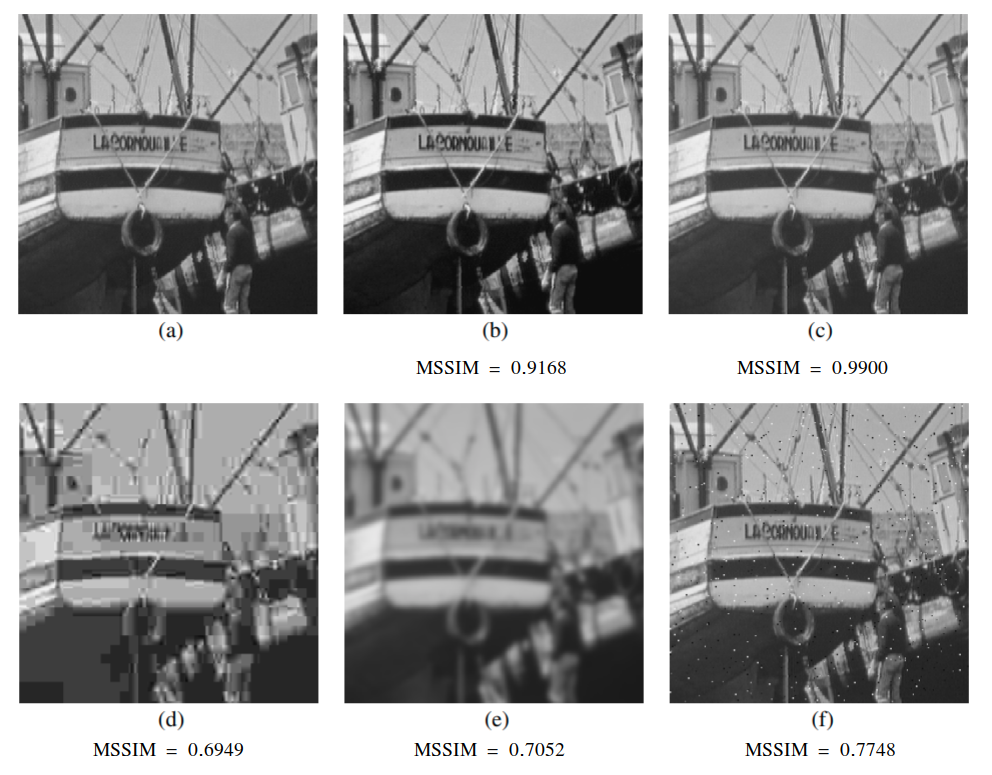
\includegraphics[scale=0.4]{images/mssim_IQA.png}
	\end{center}
	\centering
    \fdireta{wang2004image}
\end{figure}

IQA methods are also present within microscopy and its close interaction with image processing. The image acquisition in microscopy techniques may involve lasers, transmitted or reflected light, measurements of atomic force responses, the fluorescence of chemical compounds and several other means. Each technique has an inherent kind of degradation that affects the acquired images or spectra, e.g. the Raman confocal microspectroscopy suffers from the interference of cosmic rays, which yields unexpected peaks in the spectrum. Therefore, the use of IQA methods is expected. They will be investigated and used in this work. In \autoref{chapter:related-work}, some examples of NR-IQA techniques that guided the development of our method will be presented.

\section{Statistics}
Statistics is the science of planning studies and experiments, obtaining data, organizing, summarizing, presenting, analyzing, and interpreting those data and then drawing conclusions based on them; particularly among its main applications, the \emph{descriptive statistics} is a branch that comprises a set of methods which aim to describe relevant characteristics in data \cite{triola2017elementary}. The descriptive statistics methods either employ graphical elements such as boxplots, histograms, bar graphs and scatter plots to analyze data or yield numerical summary measures such as means, standard deviations, correlation coefficients and other related indices \cite{devore2011probability}. The methods that compose a descriptive statistical approach for data analysis are simple yet powerful tools that play a very important role within the scope of this project. The \emph{kurtosis} and the \emph{z-score} are the most prominent measurements for the application and will be clearly explained after some basic concepts. The graphical methods are irrelevant to this work.

Chapter~\ref{chapter:materials_and_methods} will provide information about the nature of data to be analyzed in this work. The concepts of \emph{population}, \emph{sample} and \emph{variable} are elementary: a population is a well-defined collection of objects that might be included in the analysis, a sample is a subset of a population and a variable is a feature of the objects which may change from one object to another \cite{devore2011probability}. Moreover, a \emph{frequency distribution} is a tool that presents how the data is partitioned among several categories by listing each category and its frequency of data values in each of them; a \emph{relative frequency distribution} is a frequency distribution where each frequency is represented by a proportion, usually as percentage \cite{triola2017elementary}.

\subsection{Measures of Central Tendency}

According to \citeonline{mendenhall2016statistics}, the measures of central tendency provides several ways to locate the center of the relative frequency distribution, and the three most common are the \emph{arithmetic mean}, i.e. the average of the measurements, the \emph{median}, i.e. the middle number when the measurements are ordered in ascending or descending order and the \emph{mode}, i.e. the value that occurs with the greatest frequency. Figure \ref{fig:central_tendency} presents the interpretations of these three metrics for a relative frequency distribution:

\begin{figure}[H]
	\centering
	\caption{\label{fig:central_tendency} Examples of the mean (a), median (b) and mode (c) for a relative frequency distribution.}
	\begin{center}
    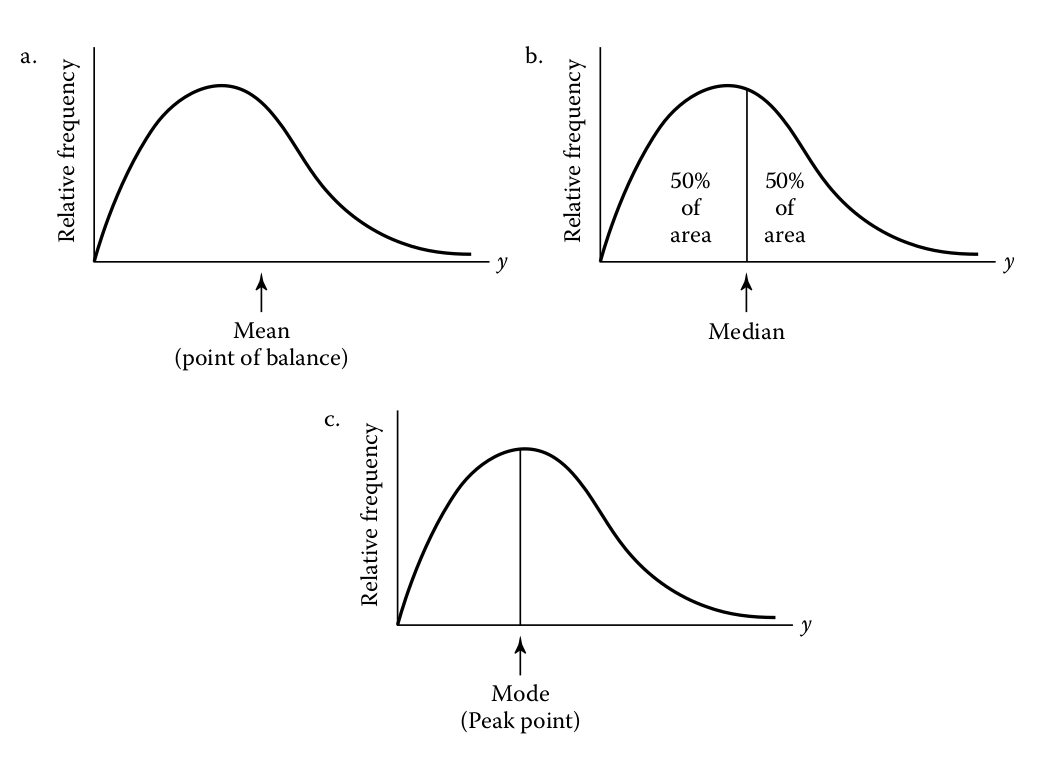
\includegraphics[scale=0.4]{images/central_tendency.png}
	\end{center}
	\centering
    \fadaptada{mendenhall2016statistics}
\end{figure}

Mathematically, the arithmetic mean is given by

\begin{equation}
\label{eqn:arithmetic_mean}
\bar{x} = \frac{1}{n} \sum_{i=1}^{n} x_{i} = \frac{x_{1} + x_{2} + \dots + x_{n}}{n},
\end{equation}

\noindent where $n$ is the sample size and $x_{i}$ represents the $i$-th observation of the variable $x$ \cite{zwillinger1999crc}.

\subsection{Measures of Variation}

The measures of variation describe how the values spread in the distribution, and commonly used measures are the range, the variance, and the standard deviation \cite{mendenhall2016statistics}. The range is simply the difference between the largest and the smallest value within the data, which may precisely point out its variability since it does not comprise the middle values among the distribution \cite{devore2011probability}. The variance measures variability based on the squared deviations about the mean and the standard deviation is the positive square root of the variance, as

\begin{align}
\label{eqn:variance_std}
\sigma^{2} = \frac{1}{n - 1} \sum_{i = 1}^{n} \left(x_{i} - \bar{x}\right)^{2}
&&
\sigma = \sqrt{\sigma^{2}},
\end{align}

\noindent where $\sigma^{2}$ and $\sigma$ are respectively the variance and the standard deviation, $x_{i}$ is the $i$-th observation of the variable $x$, $\bar{x}$ is the mean, all concerning a sample or the population \cite{zwillinger1999crc}.

\subsection{Measures of Relative Standing}

The measures of the relative standing of observations describe its locations among other values in the distribution, and two examples of these measures are \emph{percentiles} and \emph{z-scores} \cite{mendenhall2016statistics}. Percentiles are values that split the data into 100 parts in a sorted dataset, so that the $i$-th percentile stands for the $i(n + 1) / 100$ observation, e.g. the $25$-th percentile comprises $25\%$ of the data; the $z$-score, or standard score, is given by

\begin{equation}
\label{eqn:z_score}
z = \frac{x_{i} - \bar{x}}{\sigma},
\end{equation}

\noindent where $x_{i}$ is the $i$-th observation of the variable $x$, $\bar{x}$ is the mean and $\sigma$ is the standard deviation of the population or the sample \cite{zwillinger1999crc}.

\subsection{Probability Distributions}

Probability is a common and natural concept among human life, used in expressions such as ``It probably will be cold tonight''; however, there is no common formal definition accepted among statisticians and related researchers \cite{degroot2012probability}. The study of randomness, variability, and uncertainty in populations is done by analyzing probabilities, i.e. numerical descriptions of how likely an event is to occur \cite{devore2011probability}. Some basic concepts that support the probability theory are described also to the light of \citeonline{devore2011probability}, as follows:

\begin{itemize}
    \item \emph{Experiment}: Any activity or process whose outcome is subject to uncertainty;
    
    \item \emph{Sample Space}: The sample space of an experiment is the set of all possible outcomes for it;
    
    \item \emph{Event}: Any collection or subset of outcomes of a sample space;
    
    \item \emph{Random Variable}: Any rule that associates a number with each outcome in a sample space of some experiment; mathematically, it is a function with the sample space as its domain and the real numbers as its range;
    
    \item \emph{Discrete Random Variable}: A random variable with a finite set or a countably infinite sequence of possible values;
    
    \item \emph{Continuous Random Variable}: A random variable that yields zero as the probability for every possible outcome or its set of possible values is in a single interval of the real line or all numbers in a disjoint union of intervals.
    
\end{itemize}

From these concepts, it is possible to define a distribution in the scope of the probability theory. The \emph{probability distribution} is a collection of all probabilities computed from a  discrete or continuous random variable with the set of real numbers; a \emph{discrete} probability distribution is represented by the probability function itself, while a \emph{continuous} probability distribution is represented by a \sigla{p.d.f}{probability density function} \cite{mendenhall2016statistics}.

\subsection{Kurtosis}

The \emph{kurtosis} is one of the probability distribution shape statistics, which measures the extent of the peak in a distribution, i.e. its ``peakedness''; smaller absolute values indicate that the distribution tends to be uniform \cite{zwillinger1999crc}. First of all, the concepts of \emph{expectation} and \emph{moments} should be described. The expectation of a random variable (and consequently, of a distribution) is a value that summarizes its nature and is given by

\begin{align}
\label{eqn:expectation}
E(X) = \int_{-\infty}^{\infty} x p(x)dx
&&
E(X) = \sum_{x} x p(x),
\end{align}

\noindent where $x$ is each possible outcome of the random variable $X$, $p(x)$ is the probability density function for a continuous random variable (left) and the probability function for a discrete random variable (right) \cite{degroot2012probability}. Still according to \citeonline{degroot2012probability}, for a random variable $X$ and every positive $k \in \mathbb{R}$, the expectation $E(X^{k})$ is
called the $k$-th moment of $X$. The $r$-th moment may be described, according to \citeonline{zwillinger1999crc}, as

\begin{equation}
\label{eqn:rth_moment}
m_{r} = \frac{1}{n}
        \sum_{i=1}^{k}p_{i}(x_{i} - \bar{x})^{r}
\end{equation}

\noindent for every $x_{i}$ in the possible outcomes of $X$. Thus, kurtosis may be defined as the ratio of the fourth moment (equation \ref{eqn:rth_moment} with $r = 4$) by the square of the variance (also equation \ref{eqn:rth_moment} with $r = 2$), denoted by

\begin{equation}
\label{eqn:kurtosis}
g_{2} = \frac{m_{4}}{(m_{2})^{2}} - 3
\end{equation}

The $-3$ constant is due to Fischer's approach, where the kurtosis of a normal distribution is zero.

% \chapter{Related Work}
% \label{chapter:related-work}
% The concepts presented in this chapter aims to introduce a review of the literature with relevant works on blur segmentation and multifocus image fusion. The methods in both fields are somehow related, as the output of a blurry region segmentation is the input for image fusion. The blur segmentation is mostly related to transform domain methods, but some of them also have simpler mathematical tools. In a nutshell, all of them are related to the standard image processing stages: pre-processing, particular operations, feature vector extraction and analysis. 

The literature review of multifocus image fusion shows that the trend is to use either more sophisticated methods or classic and well-known methods with enhancements in order to achieve the lossless image. Instead of just creating a blur map, the fusion works aim for a specific task which will presume that the image is at its best quality possible. 

\cite{bovik2005handbook}

\section{Image Quality Assessment}

\cite{wang2004image}

% For applications in which images
% are ultimately to be viewed by human beings, the only “correct”
% method of quantifying visual image quality is through subjective evaluation. In practice, however, subjective evaluation is
% usually too inconvenient, time-consuming and expensive. The
% goal of research in objective image quality assessment is to
% develop quantitative measures that can automatically predict
% perceived image quality



\subsection{Image sharpness measure for blurred images in frequency domain}

\citeonline{kanjar2013image} proposed a Fourier Transform based algorithm to compute an image quality measure of blurred images. This approach is an attempt to quantify sharpness considering the fact that the amount of high frequency components in a blurred image is smaller than in a sharper one. The algorithm consists of the following, considering $f(x,y)$ as the input image of size $M \times N$:

\begin{enumerate}[label=\Roman*.]
    \item - Compute the Fourier Transform representation of image $f(x,y)$, denoted by $\hat{f}(m,n)$;
    
    \item - Shift the origin of the Fourier coefficients to the center of the matrix;
    
    \item - For each Fourier coefficient, compute its magnitude and assign to a matrix $A(m,n)$
    
    \begin{equation*}
        A(m,n) = \sqrt{
            [\operatorname{Re}{(\hat{f}(m,n))}]^{2}
            + [\operatorname{Im}{(\hat{f}(m,n))}]^{2}
          }
    \end{equation*}
    
    \item  Calculate the maximum value $m$ of $A(m,n)$; 
    
    \item Calculate the number $t$ of pixels in $\hat{f}$ where $\hat{f} > m /1000$;
    
    \item Calculate the image quality measure $FM = t /M.N$.
\end{enumerate}

\subsection{A no-reference perceptual blur metric}

A very simple but efficient perceptual blur metric was proposed in
\cite{marziliano2002noreference}. It is also based on the fact that high frequency components are attenuated in a blurred image. Considering that blur affects the edges and texture regions of an image, the technique attempts to measure how scattered they are. 

First, an edge detector is applied to the luminance component of the image (equivalent to a grayscale-converted image) in order to find the vertical edges. Each row of the image is scanned for pixels corresponding to edges, and the width of each edge is computed by the difference of local extrema closest to the edge. This measure is done for each edge location, and the global blur measure is the average of all computed widths.

\subsection{A No-Reference Objective Image Sharpness Metric Based on the Notion of Just Noticeable Blur (JNB)}
\label{subsec:jnb_approach}

The authors in \cite{ferzli2009noreference} utilize a psychometric model, i.e. the assignment of numerical representations to subjective tests to create an perceptual sharpness metric. The subjective tests are made concerning the \emph{Just Noticeable Blur} (JNB) concept, which is the minimum amount of perceived blurriness around an edge given a contrast higher than the limit of contrast between background and foreground that is possible to notice. 

The subjective test experiment consists in the evaluation of 27 contrast values (considering the difference between the background and the foreground grayscale values), done by 18 volunteers with normal or corrected vision, with aim to find a particular standard deviation $\sigma_{JNB}$ of a Gaussian $7 \times 7$ mask. Each contrast value yields a normalized histogram with the volunteers' responses that is treated as the probability of detecting blur in function of the standard deviation $\sigma$. The denoted by equation \ref{eqn:psychometric_jnb}:

\begin{equation}
\label{eqn:psychometric_jnb}
P = 1 - \exp{\left( - \left| \frac{\sigma}{\sigma_{JNB} } \right|^{\beta} \right)}
\end{equation}

\noindent where $\sigma$ is the standard deviation of the Gaussian blur filter and corresponds to the blur strength at the considered edge, $\sigma_{JNB}$ is the standard deviation corresponding to the JNB threshold. The parameters $\sigma_{JNB}$ and $\beta$ are chosen by means of a least-square fitting to approximate the probabilities $P$ with the answers from volunteers. The $\sigma_{JNB}$ value is adjusted to obtain $P = 63\%$.

First and foremost, the image is divided in blocks of dimensions $64 \times 64$. Let each block and the image be denoted by $R$ and $I$, respectively. All the blocks go through a Sobel edge detection process, and are later classified as “smooth” or “edge” using a threshold. If the number of edge pixels in a block is greater than $0.2\%$ of the total number of pixels in it, than it is classified as an edge block. The smooth blocks are not processed since they are not relevant in terms of blur. Than, for each block the horizontal edge pixels are retrieved and the width of each edge is computed. With this in hands, the perceptual blur metric for each block $R_{b}$ is described by equation 

\begin{equation}
\label{eqn:perceptual_blur_metric}
D_{R_{b}} = \left(
\sum_{e_{i} \in R_{b}}
\left|
\frac{w(e_{i})}{w_{JNB}(e_{i})}
\right|_{\beta}
\right)^{\frac{1}{\beta}}
\end{equation}

\noindent where $w_{JNB}(e_{i})$ is the JNB width relative to the contrast of block $R_{b}$ for all edges $e_{i}$. The parameter $\beta$ is empirically determined to be $3.4 \leq \beta \leq 3.8$ with median $3.6$. Thus, the general blur measure concerning the whole image corresponds to the probability of all blocks being blurred, given by

\begin{equation}
\label{eqn:p_blur}
    P_{blur}(I) = 1 - \Pi_{R_{b} \in I}
    \left(
    1 - P_{blur}(R_{b})
    \right)
\end{equation}

\noindent where $P_{blur}(R_{b})$ may be substituted by $1 - \exp{\left(-D_{R_{b}}^{\beta} \right)}$, which results in

\begin{align}
\label{eqn:p_blur_final}
    P_{blur}(I) = 1 - \exp{\left(-D^{\beta}\right)}
&&
D = \left(
    \sum_{R_{b}}
    \left|D_{R_{b}}
    \right|^{\beta}
    \right)^{\frac{1}{\beta}}
\end{align}

\noindent Finally, $D$ from equation \ref{eqn:p_blur_final} is then normalized by the amount of blocks an represents the final image quality index.

\subsection{A No-Reference Image Blur Metric Based on the Cumulative Probability of Blur Detection (CPBD)}

A blurriness metric that extends the approach described in \ref{subsec:jnb_approach} was proposed in \cite{narvekar2011noreference}. It is based on the cumulative probability of blur detection (CPBD), which applies the same psychometric function framework from JNB. The $w_{JNB}$ value is defined as 5 if the contrast is less or equal to 50 and 3 otherwise. The metric explores the normalized histogram of the probability of blur detection from the whole image, where CPBD is actually the percentage of edges at which blur is not likely to be detected.

First, the horizontal edges from the image are detected, also divided into blocks of $64 \times 64$ and classified as edge blocks or sharp blocks with the same threshold as in \citeonline{ferzli2009noreference}. The probability of detection blur for and edge $e_{i}$ is computed with the equation \ref{eqn:cpbd_jnb}

\begin{equation}
\label{eqn:cpbd_jnb}
\begin{split}
    P_{BLUR} &= P_{BLUR}(e_{i})\\
    &= 1 - \exp{
    \left(
        - \left|
            \frac{w(e_{i}}{w_{JNB}(e_{i})}
        \right|^\beta
    \right)}
\end{split}
\end{equation}

\noindent Then, the cumulative probability of blur detection is computed from the probability density function of equation \ref{eqn:cpbd_jnb}, and may be described as

\begin{equation}
\label{eqn:cpbd}
\begin{split}
    CPBD &= P(P_{BLUR} \leq P_{JNB})\\
    &=\sum_{P_{BLUR} = 0}^{P_{BLUR} = P_{JNB}}P(P_{BLUR})
\end{split}
\end{equation}

\noindent Thus, greater values for the CPBD metric mean sharper images.


\subsection{S3: A Spectral and Spatial Measure of Local Perceived Sharpness in Natural Images}

\citeonline{vu2012s3} proposed one technique to assess image quality that explores both spatial and spectral information from the image. The denomination $S_{3}$ represents the combination of $S_{1}$, that denotes the spectral measure of sharpness and $S_{2}$, which the authors denote as the spatial measure of sharpness. The first step is to convert the RGB image to the grayscale color space with weights $0.2989$, $0.5870$ and $0.1140$ for the red, green and blue channels, respectively. The grayscale image is then divided into blocks $\mathbf{x}$ of dimensions $m \times m$ pixels and an overlap $d$ around each neighbor block.

In order to compute the $S_{1}(\mathbf{x})$ measure, the first step is to compute the luminance contrast of each $\mathbf{x}$ block, denoted by $CR$ with the equation

\begin{align}
\label{eqn:luminance_contrast}
CR(\mathbf{x}) = l(\mathbf{x}) = \left(b + k\mathbf{x}\right)^{\gamma}
&&
b = 0.7656;\; k = 0.0364;\; \gamma = 2.2
\end{align}

\begin{align*}
\label{eqn:contrast_constraints}
CR(\mathbf{x}) = 0 \iff
    \begin{cases}
        max(l(\mathbf{x})) - min(l(x)) \leq T_{1}\\
        \mu_{1} \leq T_{2}    
    \end{cases}
&&
T_{1} = 5;\; T_{2}= 2
\end{align*}

\vspace{0.1in}

\noindent The $S_{1}$ measure for a block is set to zero if the contrast is zero. For the blocks with $CR > 0$, the magnitude spectrum is computed from the two-dimensional DFT, which is defined as the modulus of each complex coefficient and represents how much each frequency is present in the image and is represented here as $mag(\hat{\mathbf{x}})$. Then, the slope of the magnitude spectrum denoted by $\alpha_{\mathbf{x}}$ is the slope of a line in the standard form $ax + b$ and is obtained by linear regression with

\begin{equation}
\label{eqn:slope_of_magnitude}
\alpha_{\mathbf{x}} = \arg \min_{\alpha} \left\lVert \beta \hat{\mathbf{x}}^{-\alpha} -  mag(\hat{\mathbf{x}}) \right\rVert^{2}_{2}
\end{equation}

\noindent where the $L_{2}$ norm is taken over all frequencies. From this framework, $S_{1}(\mathbf{x})$ is described by

\begin{equation}
\label{eqn:sigmoid_s1}
S_{1}(\mathbf{x}) = 1 - \frac{1}{1 + e^{\tau_{1}
(\alpha_{\mathbf{x}} - \tau_{2})}}
\end{equation}

\noindent where $\tau_{1} = -3$ and $\tau_{2} = 2$. Equation \ref{eqn:sigmoid_s1} is a sigmoid function to estimate sharpness considering the slope of the spectral magnitude. This measure does not include the contrast information directly and it may generate inaccurate classifications; this is the reason why the authors propose the use of spatial information.

$S_{2}$ incorporates the spatial information by analysing the 8-neighborhoods of pixels in a block $\mathbf{x}$. The \sigla{TV}{Total Variation} is a metric of regularity within the grayscale values and is mathematically described as

\begin{equation}
\label{eqn:total_variation}
v(\mathbf{x}) = \frac{1}{255}\sum_{i,j}\left|x_{i} - x_{j}\right|
\end{equation}

\noindent where $x_{i}$ and $x_{j}$ are 8-neighbors in $\mathbf{x}$. The TV provides a good representation of the absolute differences in each block; this implies that the contrast information is consequently described well. The larger the TV index is, the higher the contrast in the block. The $S_{2}$ map is then computed as

\begin{equation}
\label{eqn:spatial_s2}
S_{2} = \frac{1}{4} \max_{a \in \mathbf{x}} v(a)
\end{equation}

\noindent where $a$ is a $2 \times 2$ block of $\mathbf{x}$. Each $x$ is of dimensions $8 \times 8$ and the overlap is $d = 4$. The final map for the whole image is the sum of all indices for each of the blocks.

Finally, let $\mathbf{X}$ denote the set of all blocks which form the image. The $S_{3}$ image quality index is the weighted geometric mean defined by

\begin{equation}
\label{eqn:s3_index}
S_{3}(\mathbf{X}) = S_{1}(\mathbf{X})^{\eta} S_{2}(\mathbf{X})^{1 - \eta}
\end{equation}

\noindent where $0 \leq \eta \leq 1$, and $\eta = 0.5$ is the best empirically obtained value for the parameter.

\subsection{A Fast Approach for No-Reference Image Sharpness Assessment Based on Maximum Local Variation}

\citeonline{bahrami2014fast} proposed the \sigla{MLV}{Maximum Local Variation} metric for image sharpness assessment. The MLV metric improves the idea of the total variation measure. Instead of computing the variations of pixel values among 8-neighborhoods, the authors propose the maximum among all differences in a neighborhood, represented by $\psi$ described by

\begin{align}
\label{eqn:mlv}
\psi(f(i,j)) = \max(f(i,j) - f(x,y))
&&
x = \{i - 1, i, i + 1\};\;\;
y = \{j - 1, j, j + 1\}
\end{align}

\noindent where $f(x,y)$ with the bounds for $x$ and $y$ denoted in equation \ref{eqn:mlv} are the 8-neighbors of the pixel $f(i,j)$. In a nutshell, the metric finds the maximum among the 8-neighborhood of a pixel, concerning the $\ell_{1}$ norm as a distance. With this setup, the algorithm begins with the grayscale conversion of an image of dimensions $M \times N$. The neighborhoods are $3 \times 3$ blocks along the image and the MLV is computed for all pixels, which results in a map $\Psi(f)$ given by

\begin{equation}
\label{eqn:mlv_matrix}
\Psi(f) =
    \begin{pmatrix}
        \psi(f(1,1)) & \cdots &  \psi(f(1,N))\\
        \vdots & \ddots & \vdots\\
        \psi(f(M,1)) & \cdots & \psi(f(M,N))
    \end{pmatrix}
\end{equation}

\noindent The next step is to apply a statistical technique to analyse how the distribution of $\Psi$ behaves when the image is sharp or blurred. For the sharp regions, i.e. high MLV values or black content, the distribution is closer to hyper-laplacian; for smoother and blurred regions, the distribution is closer to Gaussian. Therefore, the authors chose to parametrize the MLV with a \sigla{GGD}{Generalized Gaussian Distribution}, which covers the Gaussian, the laplacian and hyper-laplacian distributions and is denoted as

\begin{equation}
\label{eqn:GGD_distribution}
GGD(\Psi(f); \mu, \gamma, \sigma) =
\left(
    \frac{\gamma}{2 \sigma \Gamma \left( \frac{1}{\gamma} \right) \sqrt{\frac{\Gamma \left( \frac{1}{\gamma} \right)}{\Gamma \left( \frac{3}{\gamma} \right)}}}
\right)
e^{- \left(
        \frac{\Psi(f) - \mu}{\sigma \sqrt{\frac{\Gamma \left( \frac{1}{\gamma} \right)}{\Gamma \left( \frac{3}{\gamma} \right)}}}
    \right)^{\gamma}}
\end{equation}

\noindent where $\mu$ is the mean, $\sigma$ is the standard deviation, $\gamma$ is the shape parameter and $\Gamma(.)$ is the gamma function. In a nutshell, the MLV metric is relative to the standard deviation of the GGD distribution: the sharper the image is, the higher the standard deviation. The $\Psi$ matrix is weighted with values obtained with the exponential function $w_{i,j} = e^{\eta_{i,j}}$, where $\eta_{i,j}$ is the rank of $\psi(f(i,j))$ when sorted in ascending order.


% \section{Blur Segmentation}

% The main challenge of this project is to split the image between sharp parts and the blurred parts. The purpose of image segmentation techniques, according to \citeonline{petrou2010image}, is to extract regions that divide the image into sets of pixels with a common feature or characteristic. The extracted regions may be objects of interest for future processing or analysis. In our work, the objective is to obtain regions that were affected by the degradation process of blurring.

% In agreement with \citeonline{uma2016comparison}, the segmentation of the unfocused regions of an image may be necessary for performing post-processing and restoration processes without affecting the sharp regions. This would allow feature extraction on these clear regions, which leads to a broad variety of analysis techniques. One of the principal elements of images that loses identity with the blurring process is the edge. Regardless of properties such as thickness, shape or irregularity, the edges consist of transitions that exhibit discontinuities of intensity. Edge detectors are mathematical operations capable of retrieving such discontinuities, which are identified as blur points and contrast differences \cite{barat2004segmentation}.

% There are many techniques to obtain a map of blurry and sharp regions and many are based on solid mathematical concepts. In the next sections, the most relevant ones will be described: Haar Wavelets \cite{liang2017automatic}, Higher Order Statistics \cite{lee2014blurred}, Discrete Cosine Transform Coefficients \cite{taiebeh2017automatic} and Singular Value Decomposition \cite{su2011blurred}.

% \subsection{Wavelet-based Segmentation}

% \citeonline{liang2017automatic} proposed a Haar wavelet transform-based algorithm for blur detection and segmentation. The algorithm consists of blurring the image with a known blur kernel before performing the transform decomposition. This is due to the fact that there is a significant loss of detail after segmentation, which does not occur with such intensity if the image again undergoes a blurring process. This process can be done using a simple convolution by a Gaussian filter.

% Next, the difference between the initial image and the convolved one is estimated. The result of this operation is the partially blurred image, and the third-order transform is applied
% in blocks of 16x16 pixels around each pixel. Each block is decomposed into three sub-blocks of
% $k = \{1, 2, 3\}$ order, denoted by $\{BH_k, BV_k, BD_k \}$, which stands for horizontal, vertical and diagonals, respectively. For all orders, the $L_p$ norm of each nine components of the block, as well as the attenuation ratio $a_k$ between the components of the same block in the image test and the convolved image. The amount of blur on any pixel $(i, j)$ is given by the product of the attenuation ratios of the three orders, as presented in equations \ref{eqn:blurriness} and \ref{eqn:blurriness_norm}:

% \begin{equation}
% \label{eqn:blurriness}
% a_k(i,j) =
%     \frac
%         {
%             \Big\{
%                 ||BH_k||_p + ||BV_k||_p + ||BD_k||_p
%             \Big\}
%             \Big|_{T_r}
%         }
%         {
%             \Big\{
%                 ||BH_k||_p + ||BV_k||_p + ||BD_k||_p
%             \Big\}
%             \Big|_T
%         }
% \end{equation}

% \begin{equation}
% \label{eqn:blurriness_norm}
% a(i,j) = \prod_{k=1}^3a_k(i,j)
% \end{equation}

% The resulting $a(i, j)$ value is normalized on the $[0,1]$ interval. The closer to 1, the greater the blurriness of the block on the test image; he closer to zero, the sharper the block.

% \subsection{Higher Order Statistics-based Segmentation}

% The statistical approach to blur segmentation proposed by \citeonline{lee2014blurred} consists
% in extracting two features from the image: the \sigla{GM}{Gradient Magnitude} and the directional coherence. Higher Order Statistics based signal analysis is a tool for handling non-gaussian signals \cite{mitra2000nonlinear}. One of these techniques consists in computing the GM \cite{lee2014blurred}, that emphasizes the most intense discontinuity edges, suppresses the less intense ones and reduces noise. The framework to compute the GM is described by the equation \ref{eqn:GM} below.

% \begin{equation}
% \label{eqn:GM}
% GM(i) = \log 
%     \Bigg[
%         \frac{1}{N_{P_i}}
%             \sum_{j \in P_i} 
%             \Bigg\{\sqrt{ \frac{I_x(j)^2 + I_y(j)^2}{2}} \Bigg\}^k
%     \Bigg]
% \end{equation}

% \noindent where $I_x$ and $I_y$ are values that represent the intensity gradient in vertical and horizontal directions, respectively. $P$ represents the considered region in an iteration, centered on the $i-th$ pixel, and $N$ represents the number of pixels in $P$. The $k$ value indicates the statistical order.

% \sigla{DC}{Directional Coherence} is a measure of local similarities of a scene. It can be computed, according to \citeonline{lee2014blurred}, by applying the \sigla{ST}{Structural Tensor}, which divides the dominant directions and the coherence's directions in the local region, as depicted by equation \ref{eqn:ST}:

% \begin{equation}
% \label{eqn:ST}
% ST(i) =
%     \begin{bmatrix}
%         \sum_{j \in P_i}I_x(j)^2  & \sum_{j \in P_i}I_x(j) + I_y(j) \\
%         \sum_{j \in P_i}I_x(j) + I_y(j) & \sum_{j \in P_i}I_y(j)^2 
%     \end{bmatrix}
% \end{equation}

% \noindent ($I_x$, $I_y$, $P$ and $N$ are the same as described in Equation \ref{eqn:GM}). The eigenvalues of the ST tensor specify the degree of the anisotropy of the gradient distribution in $i-th$ region. Finally, equation \ref{eqn:DC} defines the directional coherence.

% \begin{equation}
% \label{eqn:DC}
% DC(i) =
%     \Bigg(
%         \frac{\lambda_1 - \lambda_2}{\lambda_1 + \lambda_2}
%     \Bigg)^2
% \end{equation}

% \noindent where $\lambda_{1}$ and $\lambda_{2}$ are the eigenvalues of the $ST$ matrix. After obtaining the feature vectors, it is possible to use a classifier - a function or a set of them, which labels the elements in distinct classes - and define whether each pixel is blurry or not. If prior information is provided to the classifier, it will characterize an example of supervised learning; otherwise, it will need to be able to
% infer similarities within the sample from the feature vectors, consisting in an unsupervised learning procedure. The \sigla{SVM}{Support Vector Machine} classifier can be trained and applied to determine the blurry and sharp sets of pixels.

% \subsection{Discrete Cosine Transform Coefficients Based Segmentation}

% The procedure which \citeonline{taiebeh2017automatic} proposed also takes into account the fact that blurred regions, before and after a second similar degradation process, have small differences when compared; besides, the differences between the sharp regions on the same metric are relevant. This peculiarity can also be verified in the \sigla{DCT}{Discrete Cosine Transform} domain: most of the high frequency coefficients are lost and the difference quoted above may be used to estimate the amount of blur in the image. 

% The DCT is an important mathematical operation, commonly used in data compression and signal processing, which takes sets of values and outputs transform coefficients; its two-dimensional version is executed in blocks (small sets of pixels) and is shown by equation \ref{eqn:dct} \cite{salomon2007data}:

% \begin{equation}
%     \label{eqn:dct}
%     G_{ij} = \sqrt{\frac{2}{m}}
%              \sqrt{\frac{2}{n}}
%              C_{i} C_{j}
%              \sum_{x=0}^{n-1}
%              \sum_{y=0}^{m-1}
%              p_{xy}
%              \cos 
%                 \Bigg[
%                 \frac
%                 {(2y + 1)j\pi}
%                 {2m}
%                 \Bigg]
%             \cos 
%                 \Bigg[
%                 \frac
%                 {(2x + 1)i\pi}
%                 {2n}
%                 \Bigg]
% \end{equation}

% \begin{align*}
% C_{i} =
% \begin{cases} 
%     \frac{1}{\sqrt{2}} & \text{$i = 0$,} \\
%     1 & \text{$i > 0$},
% \end{cases}
% &&
% i\in \mathbb{N} \mid 0\leq i < n
% &&
% C_{j} =
% \begin{cases} 
%     \frac{1}{\sqrt{2}} & \text{$j = 0$,} \\
%     1 & \text{$j > 0$},
% \end{cases}
% &&
% j\in \mathbb{N} \mid 0\leq j < m
% \end{align*}

% \noindent where $p_{xy}$ is the matrix which represents the image, $m$ and $n$ are the image dimensions. As described in the equation \ref{eqn:lp_norm_ratio}, the blur metric $\beta$ consists of the quotient between the $L_p$ norm of the original blurred image coefficients and the ones from the reblurred image.

% \begin{equation}
% \label{eqn:dct_image}
% 	\mathbf{D} = DCT(\mathbf{I})
% \end{equation}

% \begin{equation}
% \label{eqn:dct_reblurred_image}
% 	\mathbf{D}_b = DCT(\mathbf{I}_b)
% \end{equation}

% \begin{equation}
% \label{eqn:lp_norm_ratio}
% 	\beta(\mathbf{I}) = \frac{||\mathbf{D}_b||_p}{||\mathbf{D}||_p}
% \end{equation}

% \noindent where $\mathbf{I} \in \mathbb{R}^{2}$ is the original image and $\mathbf{I}_b \in \mathbb{R}^{2}$ is the re-blurred image with a low-pass filter (mean filter), $\mathbf{D} \in \mathbb{R}^{2}$ and $\mathbf{D}_b \in \mathbb{R}^{2}$ are the discrete cosine transforms of $\mathbf{I}$ and $\mathbf{I}_b$, respectively. The $L_p$ norm is defined by the equation \ref{eqn:lp_norm}:

% \begin{equation}
% \label{eqn:lp_norm}
% 	||\mathbf{D}_b||_p = \sum_{u,v}{(|\mathbf{D}_b(u,v)|)^p}
% \end{equation}

% \noindent The $\beta$ value is normalized on the $[0,1]$ interval; the closer to 1, the greater the amount of blur. This measurement is applied pixel by pixel in blocks of experimentally determined sizes such as 45x45, 19x19 and 9x9. The final blur measure for each pixel is an average of the measurements of the three blocks, and provide a substantially accurate blur map.

% The acquired blur map is smoothed between regions and allows to infer significant differences between the sharp and blurred ones. The segmentation process is based on the map, and uses the concept of \emph{pixon} (set of related pixels with similar properties as colour, intensity, texture, among others): the problem is based on classifying such sets of pixels. In order to create the pixel set, a blur map scan is performed in the neighbourhood of each pixel; the neighbours are joined to the pixons that have the average value closest to a certain threshold; otherwise a new pixon is created.

% The pixon set extraction divides the blur map in a set of sub-regions which will be classified as blurred or sharp. The \sigla{FCM}{Fuzzy C-Means Algorithm} was used by \citeonline{taiebeh2017automatic} and consists of the following steps:

% Let $M$ be the set of pixels with their respective intensities, $C$ be the number of classes (two, in this case) and $w\in \mathbb{R} \mid 1 < w < \infty$ be the fuzzy exponent.

% \begin{enumerate}[label=\Roman*.]

%     \item The fuzzy association functions $u_ {c, m}^{(0)}$ must be initialized with $c = {1,..., C}$ and $m = {1, ..., M}$, which are entries for an $\mathbf{U}^{(0)}$ array of $C$x$M$ dimensions;
    
%     \item For each iteration $l = {1,2,3,...,L}$, the centroids ${v_ {c}}^{l}$ of each cluster are computed by means of the equation \ref{eqn:fuzzy_cluster_center}:
    
%     \begin{equation}
%     \label{eqn:fuzzy_cluster_center}
%     	v_{c}^{l} = \frac{\sum_{m=1}^{M}(u_{c,m})^{w}x_m}{\sum_{m=1}^{M}(u_{c,m})^{w}}
%     \end{equation}

%     \item Update the $\mathbf{U}^{(l)}$ array through the equation \ref{eqn:update_matrix}:
    
%     \begin{equation}
%     \label{eqn:update_matrix}
%     	u_{c,m} = \frac{1}{\sum_{i=1}^{C}\Big(\frac{d_{c,m}}{d_{i,m}}\Big)^{\frac{2}{w-1}}}
%     \end{equation}
    
%     \noindent where $d_{i,m}^2 = ||x_m - v_i||^2$ and $||.||$ stand for the Euclidean Norm.
    
%     \item Compare $\mathbf{U}^{(l)}$ and $\mathbf{U}^{(l+1)}$. If $||\mathbf{U}^{(l)} - \mathbf{U}^{(l+1)}|| \leq \varepsilon$, the classification procedure halts; otherwise, it goes back to step II.

% \end{enumerate}

% \noindent The $w$ value determines the clustering imprecision; it has been empirically determined by the authors that $w = 2$ and $\varepsilon = 0.00005$ are appropriate choices.

% \subsection{Singular Value Decomposition-based Segmentation}

% \citeonline{su2011blurred} proposed a 
% \sigla{SVD}{Singular Value Decomposition}-based blur segmentation approach. It is a Linear Algebra derived technique of great utility, in which an array can be represented by multiple matrices of rank 1 (in this case, they can be denominated \emph{eigenimages}). The matrix equation \ref{eqn:basic_svd}
% illustrates the SVD procedure on an image.

% \begin{equation}
% \label{eqn:basic_svd}
% 	I = U{\wedge}V^{T}
% \end{equation}

% \noindent where $I$ is a matrix that represents the image, $U$ and $V$ are orthogonal arrays and $\wedge$ is a diagonal matrix, composed of multiple singular values sorted in descending order. The decomposition of the image can be represented more specifically by the equation \ref{eqn:svd}:

% \begin{equation}
% \label{eqn:svd}
% 	I = \sum_{i=1}^{n}\lambda_{i}{\mathbf{u}_i}{\mathbf{v}_i}^{T}
% \end{equation}

% \noindent where $\mathbf{u}_i$, $\mathbf{v}_i$ are column vectors of $U$ and $V$, and $\lambda_{i}$ are the diagonal terms of $\wedge$. This process decomposes the image into a weighted sum with a certain amount of eigenimages, where the weights are singular values. Image details are captured as if it was a compression procedure, in which only $k$ singular values are considered.

% Eigenimages act as multiscale analysis tools: the first most significant eigenimages involve larger scales, which provide the coarser formats; similarly, the remaining products of the decomposition provide details. Considering the convolution of a PSF $H$ with the image $I$, the high frequencies that represent the details are lost, i.e. the small singular values will correspond to larger values after the process. A blurred image has the first most significant eigen with larger singular values. The authors in \citeonline{su2011blurred} proposed a metric quantify the degree of blurriness of the image is proposed by the equation \ref{eqn:svd_blur_metric}:

% \begin{equation}
% \label{eqn:svd_blur_metric}
% 	\beta_{1} = \frac{\sum_{i=1}^{k}\lambda_{i}}{\sum_{i=1}^{n}\lambda_{i}}
% \end{equation}

% \noindent where $\lambda_{i}$ is the computed singular value for the neighbourhood of a given pixel. The metric is capable of classifying all pixels of the image in blurry or sharp with a threshold-based comparison; the result of the process is also a blur map.


\section{Multifocus Image Fusion}
\label{sec:multifocus_image_fusion}

Either in microscopic or macroscopic scales, imaging devices have a finite depth of field. All the slices of the image which are blurry came from the fact that a subset of pixels might be acquired outside the boundaries of depth of field \cite{huang2007evaluation}. Therefore, it is nearly impossible to obtain a globally sharp image in microscopic scales, since the differences of heights within the surface of the sample will also be magnified and the depth of field of microscopes is usually small in those cases. Image fusion is what may provide a fully sharp image, if a stack of images is acquired with a variety of focus adjustments.

The most trivial pixel-level fusion techniques are simple mathematical operations such as the average or a weighted average of gray levels; those are capable of performing the task, but also deliver some losses in basic image features, e.g. contrast and saturation \cite{zhang2009multifocus}. Thus, there is a demand for techniques that rely on more sophisticated tools, capable of covering multiple situations: images taken in different resolutions, light conditions and exposure times, for instance. Multiscale transform approaches, e.g. wavelet domain transforms, are a good choice for the problem and provide a very flexible framework, since it depends on the chosen wavelet function \cite{pajares2004wavelet}.

Most of the methods work upon the transform domain space, but there are also some noteworthy ones which are based on different basis. The following sections will elucidate multifocus image fusion techniques such as Graph and Spatial Frequency \cite{li2008multifocus} and Wavelet Transform \cite{pajares2004wavelet}.
% and Principal Component Analysis \cite{naidu2008pixel}.

% Nonsubsampled Contourlet Transform \cite{zhang2009multifocus}

\subsection{Graph and Spatial Frequency-based Fusion}

\citeonline{li2008multifocus} proposed an approach for the multifocus image fusion task that works on the spatial domain and has two fusion stages: the image is fused with the simple average method, then a segmentation procedure is performed by means of graph algorithms; the result is a region split of the initial images, which will be fused again with a spatial frequency technique.

Let $\mathbb{G} = (\mathbb{V},\mathbb{E})$ be the representation of a undirected weighted graph, where $\mathbb{V} = \{v_{1},v_{2},...,v_{n}\}$ is the set of vertices that stands for the pixels of the image and $\mathbb{E} = \{e_{1},e_{2},...,e_{m}\}$ is the set of edges that connect each pair of nodes based on the similarity degree shown by $\mathbf{W}(i,j)$, the weight function. The Normalized Cut algorithm is responsible for dismembering the graph into two complementary sets $A$ and $B$, and its threshold value for cutting edges is defined by equation \ref{eqn:ncut_base}

\begin{equation}
\label{eqn:ncut_base}
    Ncut = 
    \frac{cut(A,B)}{assoc(A,\mathbb{V})} +
    \frac{cut(A,B)}{assoc(B,\mathbb{V})}
\end{equation}

\noindent where $cut(A,B)$ is the sum of 
weights from $A$ to $B$, $assoc(A,\mathbb{V})$ and $assoc(B,\mathbb{V})$ are the sums of weights from $A$ an $B$ to the whole graph, respectively.

Considering $T$ as a input image, $(i,j)$ as indices for nodes, $\mathbf{F}(i)$ as intensity value for node $i$, $\mathbf{X}(i)$ as the coordinates of node $i$ and $\sigma$ as a coefficient set within 10\% and 20\% of the distance range, the proposed segmentation algorithm is organized in the following steps, as shown by \cite{li2008multifocus}:
    
\begin{enumerate}[label=\Roman*.]
    \item Build the graph with the chosen distance or similarity function and build two matrices $\mathbf{W}$ and $\mathbf{D}$, where
    
    \begin{align*}
        \mathbf{W}(i,j) = 
        \exp{\frac{-||\mathbf{F}(i)-\mathbf{F}(j)||_{2}^{2}}{\sigma_{I}^{2}}} t,
        &&
        t = 
        \begin{cases}
            \exp{\frac{-||\mathbf{X}(i)-\mathbf{X}(j)||_{2}^{2}}{\sigma_{X}^{2}}} & \text{if}
            ||X(i)-X(j)||_{2} < r
            \\0 & \text{otherwise}
        \end{cases}
    \end{align*}
    
    where $r$ is a threshold to create zeroes in $\mathbf{W}$ if the nodes have a greater distance in comparison to it and $\mathbf{D}$ is the diagonal matrix of cumulative sums for each node;
    
    \item The next step consists in computing the eigenvectors of $(\mathbf{D} - \mathbf{W})\mathbf{x} = \lambda\mathbf{D}\mathbf{x}$ with the smallest eigenvalues and minimizing the $Ncut$ function in order to perform a partition on the graph;
    
    \item Finally, check the stability of the partition by comparing the ratio between minimum and maximum of the histogram of eigenvectors values to an empirically determined threshold, $0.06$.
\end{enumerate}

With the two graph representations of image regions in hands, it is now possible to apply the spatial frequency procedure to recast the image. The metric relies on two values $RF$ and $CF$ (row frequency and column frequency), computed by equations \ref{eqn:rf} and \ref{eqn:cf}:

\begin{equation}
\label{eqn:rf}
    RF = \sqrt{\frac{1}{MN}
    \sum_{M-1}^{m=0}
    \sum_{N-1}^{n=1}
    [\mathbf{F}(m,n) - \mathbf{F}(m,n-1)]^{2}}
\end{equation}

\begin{equation}
\label{eqn:cf}
    CF = \sqrt{\frac{1}{MN}
    \sum_{N-1}^{n=0}
    \sum_{M-1}^{m=1}
    [\mathbf{F}(m,n) - \mathbf{F}(m-1,n)]^{2}}
\end{equation}

\noindent where $M$ and $N$ are the dimensions of the image and $\mathbf{F}(m,n)$ is intensity value of pixel at the position $(m,n)$. The spatial frequency is obtained by equation \ref{eqn:cf}:

\begin{equation}
\label{eqn:sf}
    SF = \sqrt{(RF)^{2} + (CF)^{2}}
\end{equation}

The spatial frequency index is then computed for every region of $A$ and $B$ subgraphs, and a decision task occurs as mathematically described in equation \ref{eqn:rof}:

\begin{equation}
\label{eqn:rof}
    RoF_{i} = 
    \begin{cases}
        RoA_{i}, & SF_{i}^{A} \geq SF_{i}^{B}\\
        RoB_{i}, & SF_{i}^{A} < SF_{i}^{B}
    \end{cases}
\end{equation}

\noindent where $i$ denotes the $i$-th region that is being calculated and the SF indices stand for correspondent regions in $A$ and $B$. If there are other images on the initial set, the process occurs in iteration for each of them.

\subsection{Wavelet Transform-based Fusion}

The modus operandi proposed by \citeonline{pajares2004wavelet} with the employment of the wavelet transform is relatively simple. It consists of applying the two-dimensional DWT in order to decompose the image in four common frequency bands for wavelet transforms as show in Figure \ref{fig:filter_banks}, where $h_{0}$ is the high band, $h_{1}$ is the low band, $f(m,n)$ is the input image and $2\downarrow$ stands for the downsampling operator that reduces the input size by half. Subsequently, there are some heuristics to merge the DWT coefficients and consequently the images.

\begin{figure}[htb]
	\centering
	\caption{\label{fig:filter_banks}Two-dimensional filter bank with four frequency bands.}
	\begin{center}
	    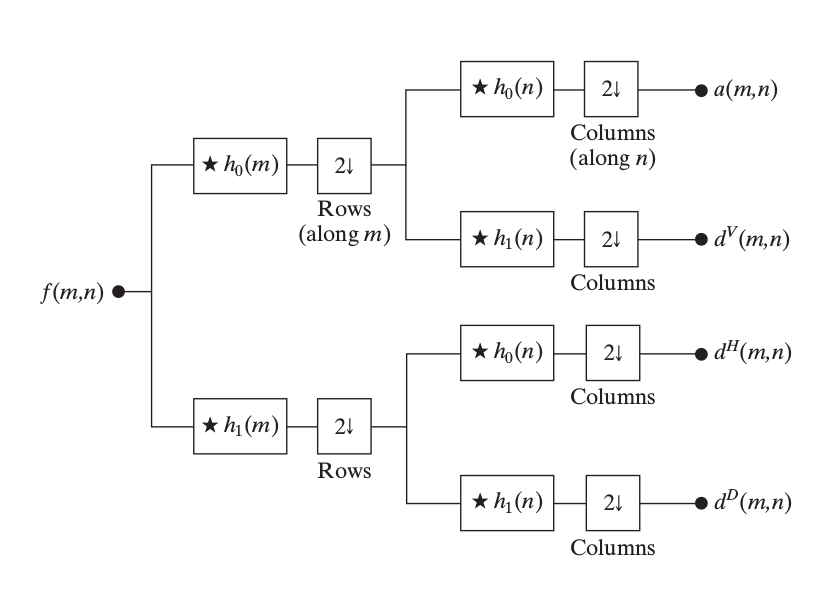
\includegraphics[scale=0.4]{images/fig11.png}
	\end{center}
	\centering
    \fdireta{gonzalez2008digital}
\end{figure}

Then, the coefficients will go through a thresholding procedure: the minimum value for taking a coefficient as significant may be obtained by the relationship of the standard deviation $\sigma$ of them all and the total size $n$ of the input: $T = \sigma\sqrt{2logn}/\sqrt{n}$. With the values from the last processing stage in hands, the fusion procedure happens with a \emph{fusion rule}, i.e. the heuristic to pick the right pixel value on each matrix in order to obtain the best fused image possible. All the values to be merged must represent the same resolution level, despite the decomposition level and the frequency band. For the multifocus image fusion, \citeonline{pajares2004wavelet} suggest the use of \sigla{CM}{Choose-Max} and \sigla{AWA}{Adaptive Weighted Average} heuristics. The CM depends on a property named activity level of the regions, represented by equation \ref{eqn:activity_level}

\begin{equation}
    \label{eqn:activity_level}
    A_{I}(p) = |D_{I}(p)|
\end{equation}

\noindent where $p = (m,n,k,l)$ is a tuple that represent a pixel in one of the decomposition levels: $m$ and $n$ indicate the spatial position in a given
frequency band, $k$ the decomposition level, and $l$ the frequency band. $D$ is a matrix with the coefficients from the decomposed image. To compute the elements that will compose the fused image, the CM procedure uses the maximum value of the same position in the two or more images, as shown by equation \ref{eqn:cm}

\begin{equation}
    \label{eqn:cm}
   CM = \max(A_{X}(p),A_{Y}(p))
\end{equation}

\noindent The AWA heuristic computes weights for each pixel with the expression in equation \ref{eqn:awa}:

\begin{equation}
    \label{eqn:awa}
   AWA = |D_{X}(p) - \Bar{D}_{X}(p)|^{a}
\end{equation}

\noindent with $\Bar{D}_{X}(p)$ representing the complementary set of positions to $D_{X}(p)$ and $a$ consisting of an exponent to modify the weight distribution. In order to finish the stack of operations and obtain the final fused image, it is only necessary to apply the \sigla{IDWT}{Inverse Discrete Wavelet Transform}.


% \chapter{Materials and Methods}
% \label{chapter:materials-and-methods}
% % The diagram on Figure \ref{fig:processing_flow} illustrates the proposed methodology to achieve the extended depth of field. The framework can be divided into four parts, as follows:

% \begin{figure}[H]
% 	\centering
% 	\caption{\label{fig:processing_flow}Generic processing flow of the extended depth of field task: Image Acquisition \textbf{(I)}, Image Pre-processing \textbf{(II)}, Image Segmentation \textbf{(III)}, Image Fusion \textbf{(IV)} and Evaluation \textbf{(V)}.}
% 	\begin{center}
% 	    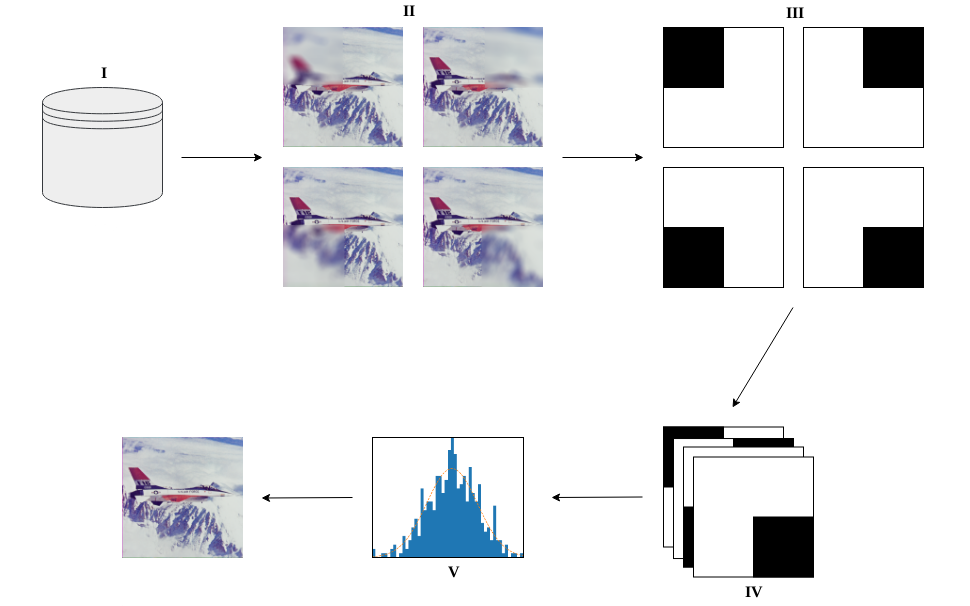
\includegraphics[scale=0.35, trim = {0 0.3cm 0 2cm}]{images/fig12.png}
% 	\end{center}
% 	\centering
%     \fautor
% \end{figure}

% \begin{enumerate}[label=\Roman*.]
%     \item \textbf{Image Acquisition}: several images will be acquired in different focus settings with the light microscope. The AxioVision 4.8 acquisition module tool called \emph{Z-Stack} allows to acquire images along the $z$ axis with a motorized focusing device that provides steps between each image with micrometer scale precision. This will result in a set of images with different levels of blur;
    
%     \item \textbf{Image Pre-processing}: some adjustments are necessary prior to segmentation. The original image stack is in the RGB colour space. There was a conversion to colour spaces such as the \sigla{HSV}{Hue, Saturation and Value colour space}, in which the Value channel may be used for processing, the \sigla{LAB}{Lightness and colour-opponent dimensions A and B} where the Lightness channel could be processed or just a conversion from RGB to grayscale in order to perform tests. This process is reversible, so that images can be presented in their original RGB colour space;
    
%     \item \textbf{Image Segmentation}: images will go through a process of splitting the pixels in blurred and sharp groups. This step will locally scan the pixels in some transform domain (\textit{a priori}, in the Fourier domain) in order to label them in one of the groups. In a nutshell, this will either produce a matrix of zeros and ones with the same dimensions of the image, or a set of regions labeled as blurry or sharp (which depends on the chosen window size for STFT, for example). This represents the blur maps and will work as input to carry out the fusion step;
    
%     \item \textbf{Image Fusion}: the step consists of scanning the blur maps and selecting the sharp regions in each image; these will be merged so as to minimize overlaps, and the final result will be a mostly or fully sharp image. The blur maps contain information about each sharp region of each image, and the image fusion process will choose the sharpest pixels to compose the resulting image based on the blur map and a numerical metric; the former may be based on pixel-level or transform domain level approaches.
    
%     \item \textbf{Evaluation}:  evaluate the quality of the segmentation procedure and also compare the sharpness level of the fused image with other images. This will allow to gauge the reliability of the processes and determine whether a) the process should be repeated; b) the parameters of the algorithms are well estimated and c) the algorithm itself is performing well. The final image fusion result will be evaluated with error-based methods and the segmentation quality will have probability measurements of precision, in comparison to the ground truth images. 
% \end{enumerate}

% The next sections will provide details on the data to be processed and relevant information on the techniques that will be used to fulfill the proposal.

% \section{Materials}

% To precisely validate the segmentation process, a set of \emph{ground truth} images with structures of well-known dimensions, formats and known blurry regions is required. This can be done by imaging a set of objects such as coins, crystals and stones. It is also possible to blur sharp structures by the convolution of a known blur kernel with a sharp image. 

% This can be directly applied in order to obtain higher quality in plant leaf histological samples, which have a specific structured called \emph{stoma}, responsible for gas exchanges with the surrounding medium. \emph{Stomata} exhibit a non-regular topology which leads to defocus blur while acquiring images. There are several works on plant leaf images done by the  \sigla{SCG}{Scientific Computing Group} in \sigla{IFSC}{São Carlos Institute of Physics}, including biological studies with complex network analysis, as the stomata were modelled as graphs. Figure \ref{fig:validation_images} shows how the test images may look like:

% \begin{figure}[htb]
% 	\centering
% 	\caption{\label{fig:validation_images}Images that may be used for evaluating the algorithm: (a) partially blurred airplane with an artificial gaussian blur kernel, (b) a 300x magnified contact pad for the electrical interface on the front side of a credit card , (c) surface of a 300x magnified Brazilian 5 \emph{centavos} coin and (d) 50x magnified \textit{Callisia repens} specimen, where it is possible to see stomata and a blurry background.}
% 	\begin{center}
% 	    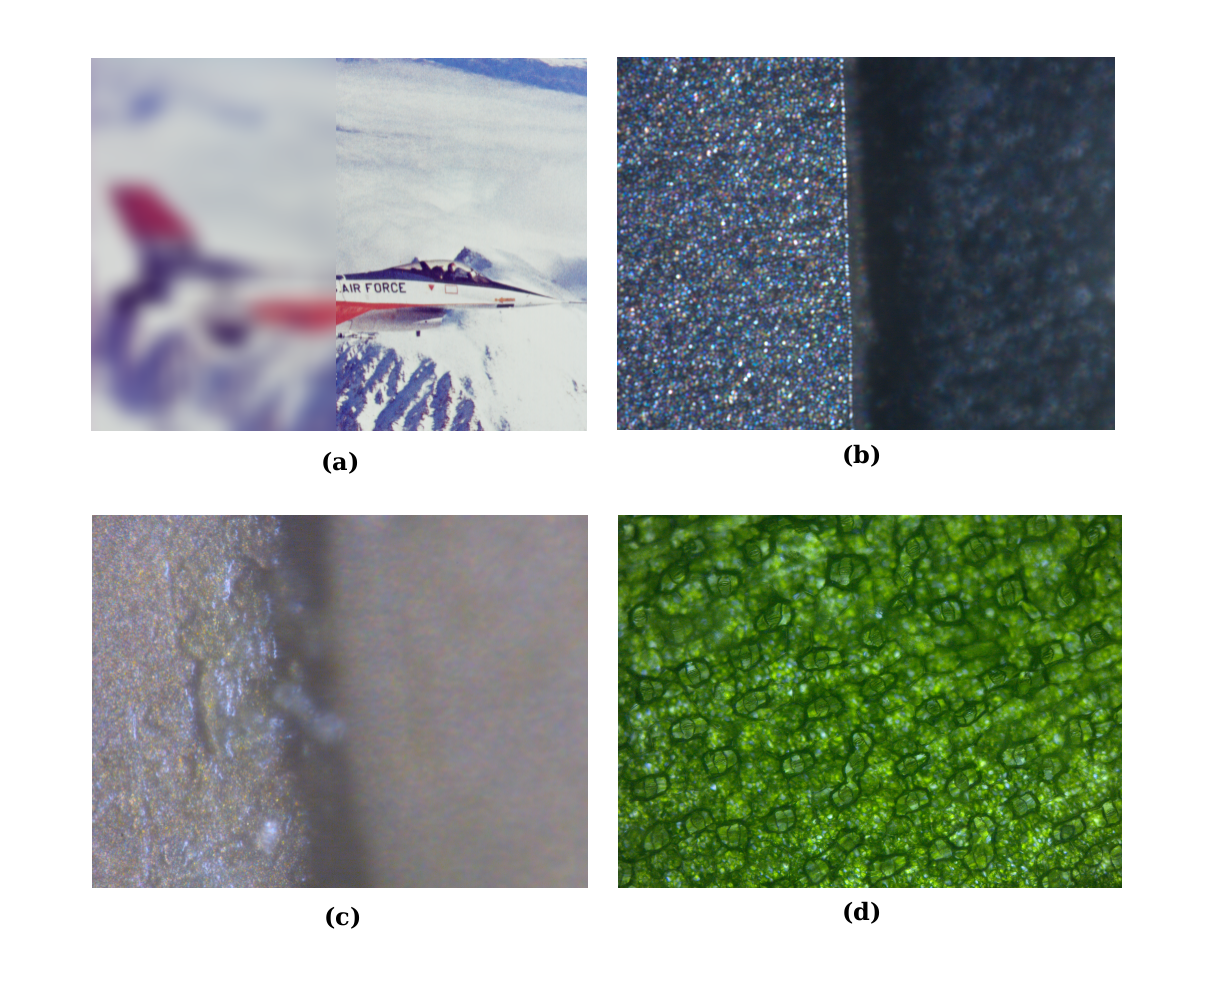
\includegraphics[scale=0.35]{images/fig13.png}
% 	\end{center}
% 	\centering
%     \fautor
% \end{figure}

% The images will be acquired with a ZEISS SteREO Discovery.v20 stereo compound microscope. This microscope is used for three-dimensional observations of small objects, with applications in biology, medicine and tissue examination \cite{stereo2012carl}. Figure \ref{fig:stereo_v20} illustrates a stereo compound light microscope from the SCG group that was used to obtain images \ref{fig:validation_images}.\textbf{(b)}, \ref{fig:validation_images}.\textbf{(c) }and \ref{fig:validation_images}.\textbf{(d)}.

% \begin{figure}[H]
% 	\centering
% 	\caption{\label{fig:stereo_v20}Zeiss SteREO v20 microscope from the SCG group.}
% 	\begin{center}
% 	    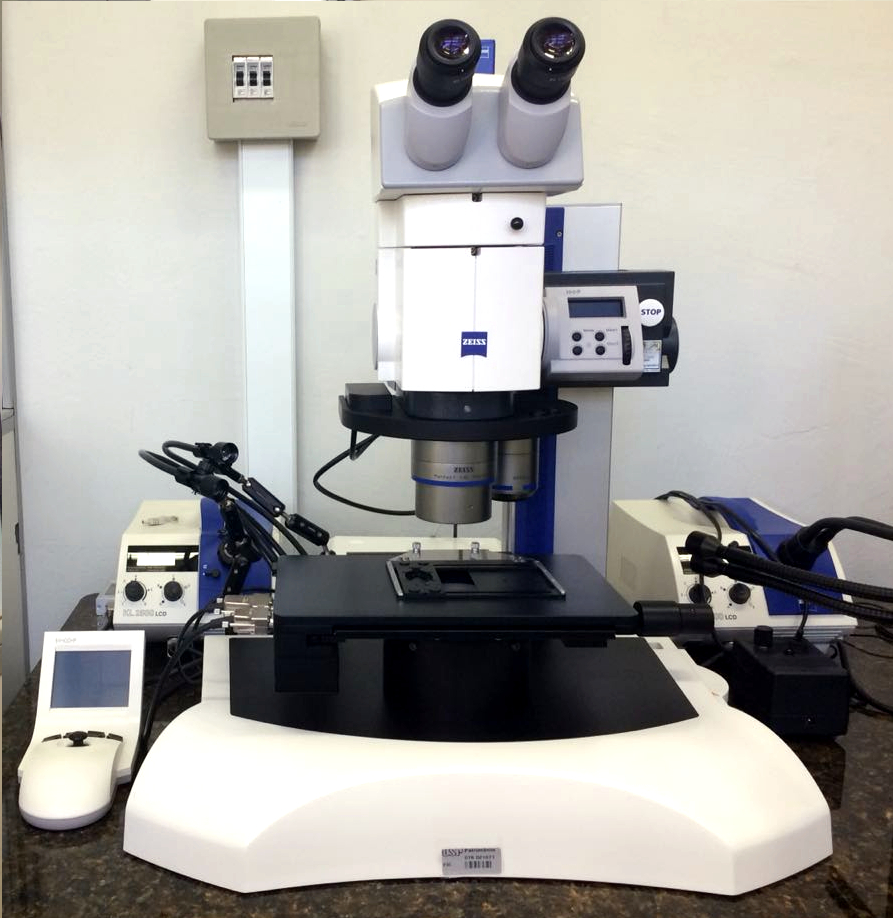
\includegraphics[scale=0.3]{images/fig14.png}
% 	\end{center}
% 	\centering
%     \fautor
% \end{figure}

\section{Methods}

\subsection{Discrete Fourier Transform based no-reference image quality assessment}
teste

% One of the pre-processing tasks consists of colour space conversion, from RGB to HSV and LAB , or to grayscale for testing purposes only. A noise reduction procedure may also be necessary, since microscopy images have a considerable amount of noise. If the amount of noise is created by the texture of the surface, e.g. the coin surface, which shows a particle pattern when magnified, noise reduction procedures should not be done as pre-processing.

% According to the literature review from chapter \ref{chapter:related-work}, both segmentation and fusion procedures depend on the problem and should have their parameters optimized empirically. There are several approaches applied by image segmentation algorithms such as pixel-level analysis, region based segmentation, edge based segmentation and so on. Those which are done in the spatial domain have a high computational cost and also a high computational complexity, and are designed for tasks where the segmentation appears to be simple. For region-based segmentation, there are techniques that rely on other mathematical frameworks, e.g. transform domain methods, statistical analysis and linear algebra, as shown in chapter \ref{chapter:related-work}. This work proposes a region-based image segmentation method within transform domains.

% The first proposed method for blur segmentation lies upon FFT analysis to identify images with low degree of blur. The most trivial method to be tested is the computation of spectral energy density in frequency bands of the global FFT. The energy in this contexts is somehow related to its concept is physics: the amount of some quantity that should be transferred to something in order to promote the increase or decrease of some property, e.g. the transfer of heat in order to increase the temperature. In this case, spectral energy density consists of the frequency response of the amount of photons which were transferred to the sensor when the image was acquired. The energy can be computed with the $L_{2}$ norm as described in equation \ref{eqn:spectral_energy_density}:

% \begin{equation}
% \label{eqn:spectral_energy_density}  
%     E = \sum_{x=0}^{M-1}\sum_{y=0}^{N-1}|F(x,y)|^{2}
% \end{equation}

% \noindent where $F$ is the FFT coefficients from the transformed image, $M$ and $N$ are the dimensions of the spectrum. The frequency bands, considering the shift of smallest coefficients to the center of the spectrum, the center as an origin for a coordinate system and the image dimensions as $N$x$N$, consists of lower frequencies in circles around the center (with radius $r < N/2$), medium frequencies when $r$ is close to $N/2$ and high frequencies when $r > N/2$. The idea is that blurry images have spectral energy density values with lower magnitudes, since the blurring process promotes a loss of details and is similar to low-pass filtering operation.

% The acquisition of the different bands in two-dimensional spectra can be made with circles centered at the zero frequency, shifted to the image central coordinate. Alternatively, the use of rectangles (or frames) may have similar effects due to the fact that the spectrum can be taken as a mixture of two one-dimensional spectra in each axis. In the end of the process,  images can be taken as sharp or blurry, considering the magnitude of the energy values.

% Following this approach, the next trial is to apply the two-dimensional STFT and also compute the energy in different bands. It is known that microscopy images suffer partial blur due to the depth of field feature. Therefore, local analysis may be used to obtain a precise blur map. The algorithm for computing the transform consists of the following steps:

% \begin{enumerate}[label=\Roman*.]
%     \item Generate a discrete two-dimensional window from two one-dimensional windows. The lengths of each window are taken as input, but it is mandatory that their dimensions originate a window that fits into the image;
    
%     \item Separate the image in slices of the same dimensions of the window. For each slice, perform the inner product between the image and the window;
    
%     \item For each windowed slice, perform the FFT.
% \end{enumerate}

% The result is a set of local FFTs. For blurred slices, higher energy values within the low--mid bands will be expected. 

% The next step is the image fusion. According to \citeonline{garg2014survey}, the spatial domain-based algorithms cause blur and are sensitive to noise, but contain reasonable information about positions of objects in the scene. Transform domain-based solutions are more complex to implement and also have a higher computational complexity in comparison its counterpart. Therefore, transform domain techniques alone, or a combination of both,  is suitable for this work.

% The proposed image fusion algorithm is based on the Fourier domain. Since the proposed segmentation procedure provides a blur map and transforms the image from the spatial domain to the Fourier domain, it is possible to use the information of the blur maps and also the remaining coefficients from the transform in order to perform image fusion. Considering that each coefficient represents a pixel in the original image, the image slices from the STFT on each of the multifocus images can be considered as a \emph{tensor} (a higher dimension array in this case). Figure \ref{fig:tensor} denotes a simple example of the tensor concept:

% \begin{figure}[H]
% 	\centering
% 	\caption{\label{fig:tensor}Graphical idea of a $8$x$8$x$8$ tensor, which arbitrarily represents the structure of the blur maps and the resulting Fourier spectra from the segmentation procedure.}
% 	\begin{center}
% 	    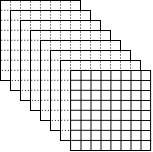
\includegraphics[scale=0.8]{images/fig15.png}
% 	\end{center}
% 	\centering
%     \fautor
% \end{figure}

% \noindent For each pixel of the image, which corresponds to one complex coefficient in one of the Fourier spectra, the average of the values should be calculated and the coefficient with the highest similarity will be chosen as the corresponding pixel to compose the fused image. If a set of coefficients has the same similarity when compared to the average value, it means that all related pixels have the same degree of sharpness, then the coefficient may be randomly chosen. 




% \section{Evaluation Methods}

% According to \citeonline{bovik2009mean}, the \sigla{MSE}{Mean Squared Error} is a measure of signal fidelity. Two signals are compared and a quantitative measure that describes the degree of similarity (fidelity), or the degree of error between them is computed. One indicator is considered as ideal and the other as a result of processes that may have distortions and inconsistencies. Considering $f (x, y)$ and $g (x, y)$ as two functions, the MSE can be represented by the equation \ref{eqn:mse}, and in a general way by equation \ref{eqn:mse_lp_norm}:

% \begin{equation}
% \label{eqn:mse}
% 	MSE =  \frac{1}{MN}\sum_{i=1}^{M}\sum_{j=1}^{N}(f(x,y) - g(x,y))^2
% \end{equation}

% \begin{equation}
% \label{eqn:lp_norm2}
% 	d_p(f,g) = \Bigg(\sum_{i=1}^{M}\sum_{j=1}^{N}|f(x,y) - g(x,y)|^{p}\Bigg)^{1/p}
% \end{equation}

% \begin{equation}
% \label{eqn:mse_lp_norm}
% 	MSE =  \frac{1}{MN}d_p(f,g)
% \end{equation}

% \noindent where $M$ and $N$ are the dimensions of both signals and $p$ is the $l_{p}$ norm value, defined as distance function $d:S$ x $S \rightarrow \mathbb{R}^2$. An important derivation of this measure is the RMSE, which is just the root square of the MSE value and changes the range of the metric. For image processing, the MSE is converted into the PSNR metric, which is defined by the equation \ref{eqn:psnr}:

% \begin{equation}
% \label{eqn:psnr}
% 	PSNR = 10\log_{10}\Bigg(\frac{L^2}{\sqrt{MSE}}\Bigg)
% \end{equation}

% \noindent where $L$ is the intensity range for each pixel, usually $[0,255]$.

% The resulting blur map from the segmentation process is an array with binary values; it is possible to quantitatively determine the reliability of the segmentation. According to \citeonline{choi2009survey}, the binary feature vector is one of the most common pattern representations, and the similarity and distance measures performed in these sets of information are important for grouping, sorting and analysing data.

% Two common similarity metrics, the Jaccard and Dice indices, are appropriate in this scenario. Both are comprised within the $[0,1]$ interval, where 1 is the complete similarity and 0 the complete discrepancy. Table \ref{tab:jaccard_contingency} represents the relationship between the presence and absence of the pixels in two sets A (ground truth segmentation) and B (segmented image).

%         \begin{table}[!hbt]
% 		% Center the table
% 		\begin{center}
% 		% Title of the table
% 		\caption{Contingency table for Jaccard and Dice similarity indices.}
% 		\label{tab:jaccard_contingency}
% 		% Table itself: here we have two columns which are centered and have lines to the left, right and in the middle: |c|c|
% 		\begin{tabular}{|c|c|c|c|}
% 			% To create a horizontal line, type 
%             \hline
%              & Presence (A) & Absence (A) & $\mathit{\sum}$\\
%     		\hline
%           	 Presence (B) & a & b & a + b\\
%     		\hline
%           	 Absence (B) & c & d & c + d\\
% 			\hline
%              $\mathit{\sum}$ & a + c & b + d & a + b + c + d\\
%             \hline
% 		\end{tabular}
% 		\end{center}
% 		\fautor
%       \end{table}
      
% In this work, $a$ is the number of pixels classified as blurred in both sets, $b$ is the number of pixels classified as blurred in B but not in A, $c$ is the number of pixels classified as blurred in A but not in B, and $d$ is the number of pixels classified as sharp in both sets. As a result, the Jaccard and Dice similarity indices can be described by the equations \ref{eqn:jaccard} and \ref{eqn:dice}, respectively:

% \begin{equation}
% \label{eqn:jaccard}
% 	S_{jaccard} = \frac{a}{a + b + c}
% \end{equation}

% \begin{equation}
% \label{eqn:dice}
% 	S_{dice} = \frac{2a}{2a + b + c}
% \end{equation}

% \chapter{Results}
% \label{chapter:results}
% % Experiments for the segmentation procedure were carried out for the two proposed methods: a) FFT and b) STFT. The proposed image sets were built in order to perform tests with real multifocus microscopy images with their own point spread function and defocus blur feature. The coin images were acquired with 300x magnification,  5 $\mu m$ Depth of Field and 10 $\mu m$ step between each image on the $z$ axis. Two different slopes between the coin letters were considered: the slope between the background of the coin and the "o" letter and the same approach for the 90 degrees rotated "v" letter in the Portuguese word \emph{centavos} of the coin, shown in figure \ref{fig:original_coin}. The slope on the images was made on purpose for creating a very pronounced blur effect with the differences in the microscope objective's height. Ten images were taken from the "o" and "v" slopes. The blurred parts are known to be either \emph{left} or \emph{right}, as summarized by table \ref{tab:coin_card_set_description} and shown in figure \ref{fig:card_coin_images}:

% \begin{figure}[H]
% 	\centering
% 	\caption{\label{fig:original_coin}10-\emph{cent} Brazilian Real coin.}
% 	\begin{center}
% 	    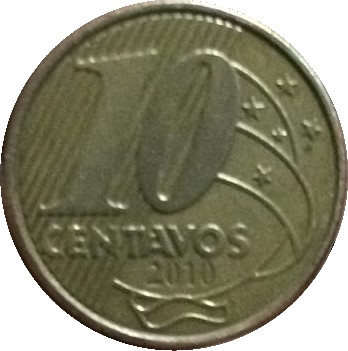
\includegraphics[scale=0.5, trim = {0 0 0 1cm}]{images/fig16.png}
% 	\end{center}
% 	\centering
%     \fautor
% \end{figure}

% \begin{table}[H]
%     \centering
%     \caption{Description of the sharp parts of the image sets (a) coin "o" letter and (b) coin "v" letter.}\label{tab:coin_card_set_description}
%     \begin{subtable}{.35\linewidth}
    
%     %Center the table
% 		\begin{center}
% 		% Title of the table
% 		\caption{}
%         \begin{tabular}
%         {|c|c|c|}
%         \hline
        
%             % header
%             Image & Sharp Part
%             \\ \hline
%             % data
%             coin "o" 1 & None
%             \\ \hline
            
%             coin "o" 2 & None
%             \\ \hline
            
%             coin "o" 3 & Left
%             \\ \hline
            
%             coin "o" 4& Left
%             \\ \hline
            
%             coin "o" 5 & Left
%             \\ \hline
            
%             coin "o" 6 & Right
%             \\ \hline
            
%             coin "o" 7 & Right
%             \\ \hline
            
%             coin "o" 8 & None
%             \\ \hline
            
%             coin "o" 9 & None
%             \\ \hline
            
%             coin "o" 10 & None
%             \\ \hline
            
%         \end{tabular}
%     \end{center}
%     \end{subtable}%
%     \begin{subtable}{.35\linewidth}

%         %Center the table
% 		\begin{center}
% 		% Title of the table
% 		\caption{}
%         \begin{tabular}
%         {|c|c|c|}
%         \hline
        
%             % header
%             Image & Sharp Part
%             \\ \hline
%             % data
%             coin "v" 1 & None
%             \\ \hline
            
%             coin "v" 2 & None
%             \\ \hline
            
%             coin "v" 3 & Right
%             \\ \hline
            
%             coin "v" 4& Right
%             \\ \hline
            
%             coin "v" 5 & Right
%             \\ \hline
            
%             coin "v" 6 & Right
%             \\ \hline
            
%             coin "v" 7 & Left
%             \\ \hline
            
%             coin "v" 8 & Left
%             \\ \hline
            
%             coin "v" 9 & Left
%             \\ \hline
            
%             coin "v" 10 & Left
%             \\ \hline
            
%         \end{tabular}
%     \end{center}
%     \end{subtable} 
%     \hspace{0.8cm}
%     \fautor
% \end{table}

% \begin{figure}[H]
% 	\centering
% 	\caption{\label{fig:card_coin_images}Samples from the coin and card image sets: (a) and (b) left and right sharp sides of coin "o" letter, respectively, (c) and (d) left and right sharp sides of coin "v" letter, respectively.}
% 	\begin{center}
% 	    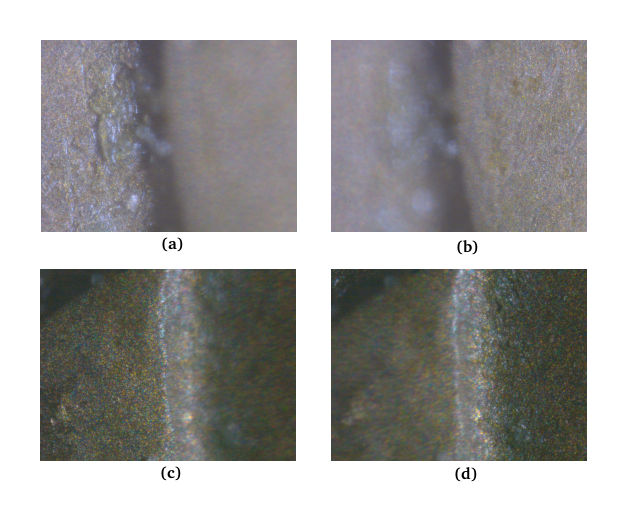
\includegraphics[scale=0.6, trim = {0 1cm 0 1cm}]{images/fig17.png}
% 	\end{center}
% 	\centering
%     \fautor
% \end{figure}

% \noindent An analogous image set for testing purposes was created, i.e. the card. It consists of images of a contact pad for the electrical interface of a bank card. It was chosen because of a coarser slope when compared to the coin images. The images were acquired also with 300x magnification, a 5 $\mu m$ Depth of Field and a 10 $\mu m$ step between each image on the $z$ axis. Some samples of the card image set are denote by figure \ref{fig:card_set_images} and the description of the card set can be seen in table \ref{tab:card_set_description}.

% \begin{figure}[H]
% 	\centering
% 	\caption{\label{fig:card_set_images}Card contact pad images: contact pad (a), left and right sharp sides (b) .}
% 	\begin{subfigure}{.5\textwidth}
%         \centering
%         \frame{
\includegraphics[scale=1]{images/fig18a.png}}
%         \caption{}
%     \end{subfigure}\\
%     \begin{subfigure}{\textwidth}
%          \centering
%          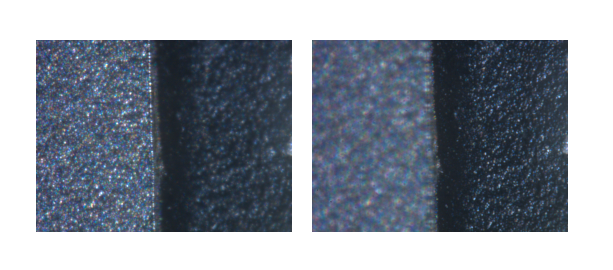
\includegraphics[scale=0.5, trim = {0 0cm 0 0cm}]{images/fig18b.png}
%          \caption{}
%     \end{subfigure}
% 	    \fautor
% \end{figure}


% \begin{table}[htb]
%     \centering
%     \caption{Description of the sharp parts of the card image set.}\label{tab:card_set_description}
%     %Center the table
% 		\begin{center}
% 		% Title of the table
%         \begin{tabular}
%         {|c|c|c|}
%         \hline
%             % header
%             Image & Sharp Part
%             \\ \hline
%             % data
%             card 1 & None
%             \\ \hline
            
%             card 2 & None
%             \\ \hline
            
%             card 3 & Left
%             \\ \hline
            
%             card 4& Left
%             \\ \hline
            
%             card 5 & Left
%             \\ \hline
            
%             card 6 & Left
%             \\ \hline
            
%             card 7 & Right
%             \\ \hline
            
%             card 8 & Right
%             \\ \hline
            
%             card 9 & Right
%             \\ \hline
            
%             card" 10 & Right
%             \\ \hline
            
%             card" 11 & None
%             \\ \hline

%             card" 12 & None
%             \\ \hline
            
%         \end{tabular}
%     \end{center}
%     \fautor
% \end{table}

% An artificially blurred image was also used for the tests. The airplane image consists of an common standard $256$x$512$ test image of an F-16 airplane, obtained from the \sigla{USC-SIPI}{University of Southern California - Signal and Image Processing Institute} image databases \cite{uscsipi1977image}. The blurring process consisted of dividing the image in two halves (left and right) with $256$x$512$ pixels each and blurring the left one with a Gaussian Blur Kernel of radius $30$ with the aid of \sigla{GIMP}{GNU Image Manipulation Program}. This image set is shown in figure \ref{fig:airplane_set_images}:

% \begin{figure}[H]
% 	\centering
% 	\caption{\label{fig:airplane_set_images}Airplane contact pad images: left (a) and right (b) sharp sides.}
% 	\begin{center}
% 	    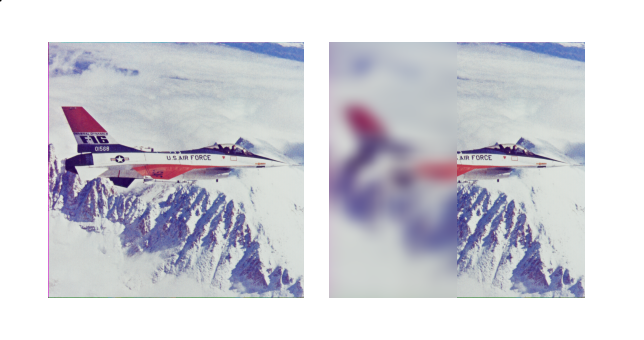
\includegraphics[scale=0.6, trim = {0 1cm 0 1cm}]{images/fig19.png}
% 	\end{center}
% 	\centering
%     \fautor
% \end{figure}

% \section{FFT Test}
% \label{sec:fft-test}

% As expected, the global approach is capable of electing the mostly sharp image within a set of partially blurred images. The magnitude of the spectral energy density values was higher for the sharper images, mostly the ones which have a sharp side, either left or right. Three frequency bands were considered to compute the results: \emph{mid}, \emph{high} and \emph{highest}. The computation of the bands was done in the three proposed colourspaces, and the grayscale one was the most precise. Comprehensive results for grayscale and other colourspaces are shown in appendix \ref{chapter:fft-test-results}. Notice that this approach is not capable of precisely pointing out the location of the blurry parts of the image. Figure \ref{fig:fft_results} presents the frequency band energy values with the grayscale colourspace on each band for the FFT approach. The amount of bar triads is related to the amount of images in the set: for the coin "o" and coin "v" images, 10 bar triads were shown; analogously, 12 for the card set and 2 for the airplane set.

% \begin{figure}[H]
%     \centering
%     \caption{\label{fig:fft_results}Grayscale colourspace FFT approach for coin "o" (upper left), coin "v" (upper right), card (lower left) and airplane (lower right) images.}
%     \subfloat{
%         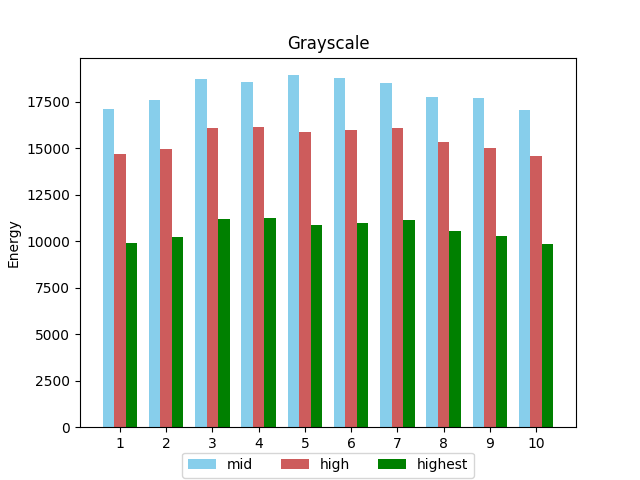
\includegraphics[width=0.45\textwidth]{images/fig20a.png}
%         \label{fig:subfig1}
%     }
%     \qquad
%     \subfloat{
%         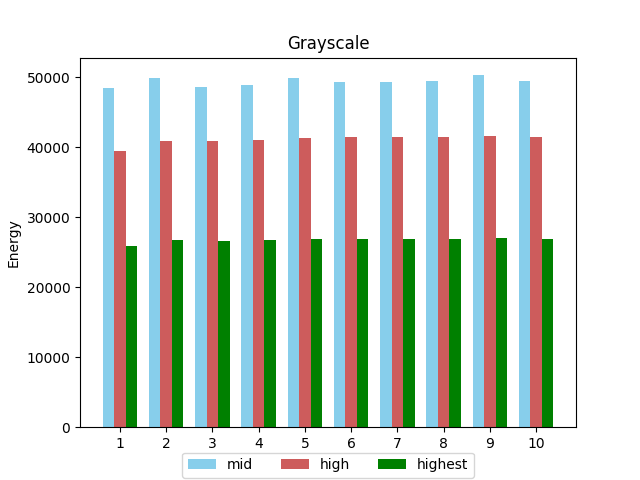
\includegraphics[width=0.45\textwidth]{images/fig20b.png}
%         \label{fig:subfig2}
%     }
%     \subfloat{
%         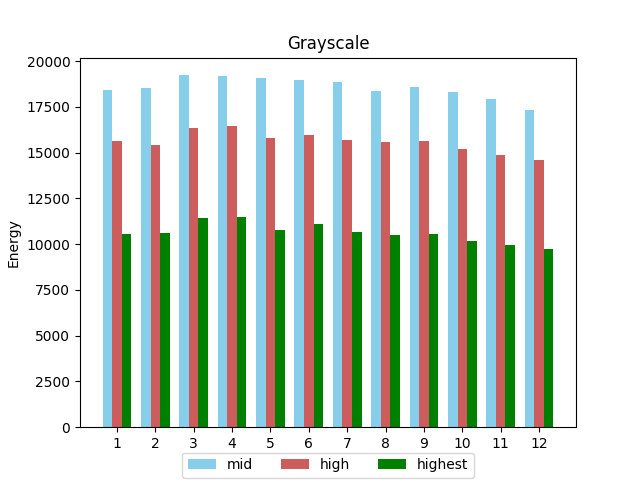
\includegraphics[width=0.45\textwidth]{images/fig20c.png}
%         \label{fig:subfig3}
%     }
%     \qquad
%     \subfloat{
%         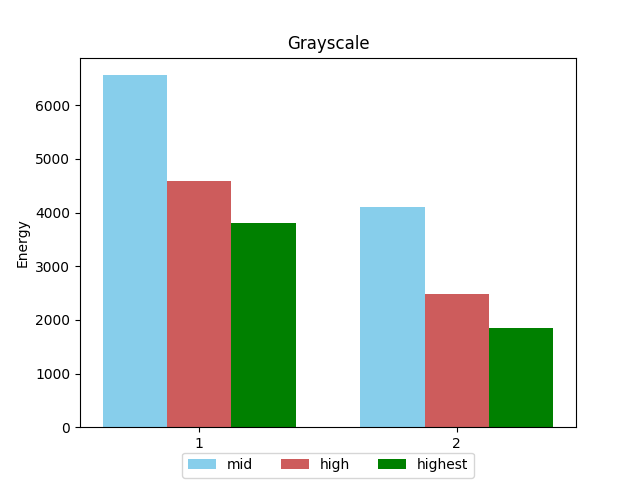
\includegraphics[width=0.45\textwidth]{images/fig20d.png}
%         \label{fig:subfig4}
%     }
%     \hspace{1cm}
%     \fautor
% \end{figure}

% \section{STFT Test}

% The Short-time Fourier Transform approach presented relevant results concerning the information about the amount of blur on each region of the images. The test cases were made in such a way that positive results should be expected: the most efficient window size was already set due to the prior knowledge about the blurry and the sharp regions. With the same configuration for colourspaces and frequency bands, the test were done with several different window functions that are printed on the appendix \ref{chapter:stft-test-results}. The figures \ref{fig:stft_card}, \ref{fig:stft_coin_o}, \ref{fig:stft_coin_v} and \ref{fig:stft_airplane} presents the frequency band energy values with the grayscale colourspace on each band for the STFT approach, with the Hann window function, for the left and right sections (left and right in the airplane graph and \emph{L} and \emph{R} for the other graphs). The graphs stand for the card, coin "o", coin "v" and airplane image sets, respectively. The bar triad settings are the same as in section \ref{sec:fft-test}.


% \begin{figure}[ht]
% 	\centering
% 	\caption{\label{fig:stft_card}Grayscale colourspace STFT approach for card images.}
% 	\begin{center}
% 	    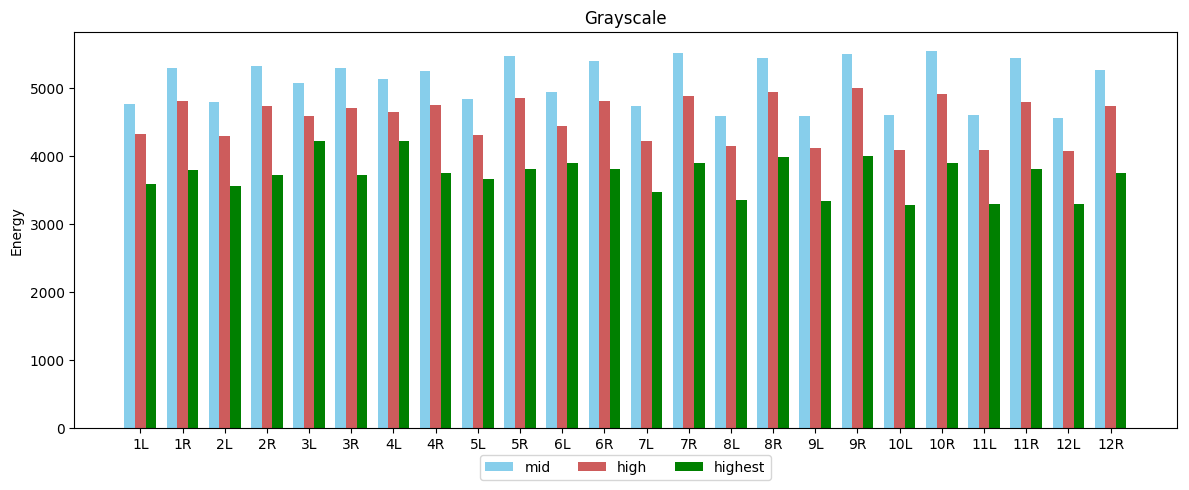
\includegraphics[scale=0.52, trim = {0 1cm 0 1cm}]{images/fig21.png}
% 	\end{center}
% 	\centering
%     \fautor
% \end{figure}

% \begin{figure}[ht]
% 	\centering
% 	\caption{\label{fig:stft_coin_o}Grayscale colourspace STFT approach for coin "o" images.}
% 	\begin{center}
% 	    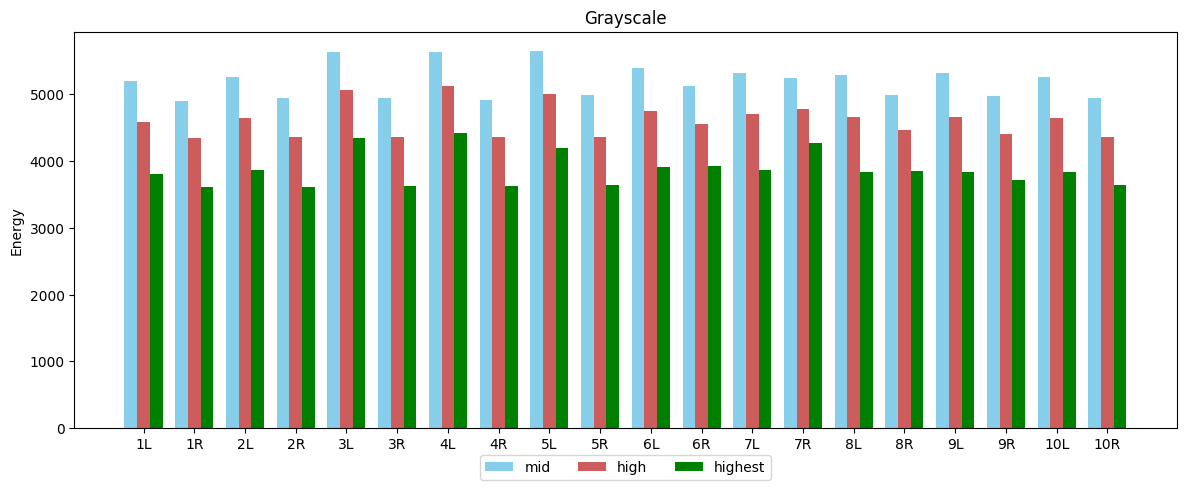
\includegraphics[scale=0.52, trim = {0 1cm 0 1cm}]{images/fig22.png}
% 	\end{center}
% 	\centering
%     \fautor
% \end{figure}

% \begin{figure}[ht]
% 	\centering
% 	\caption{\label{fig:stft_coin_v}Grayscale colourspace STFT approach for coin "v" images.}
% 	\begin{center}
% 	    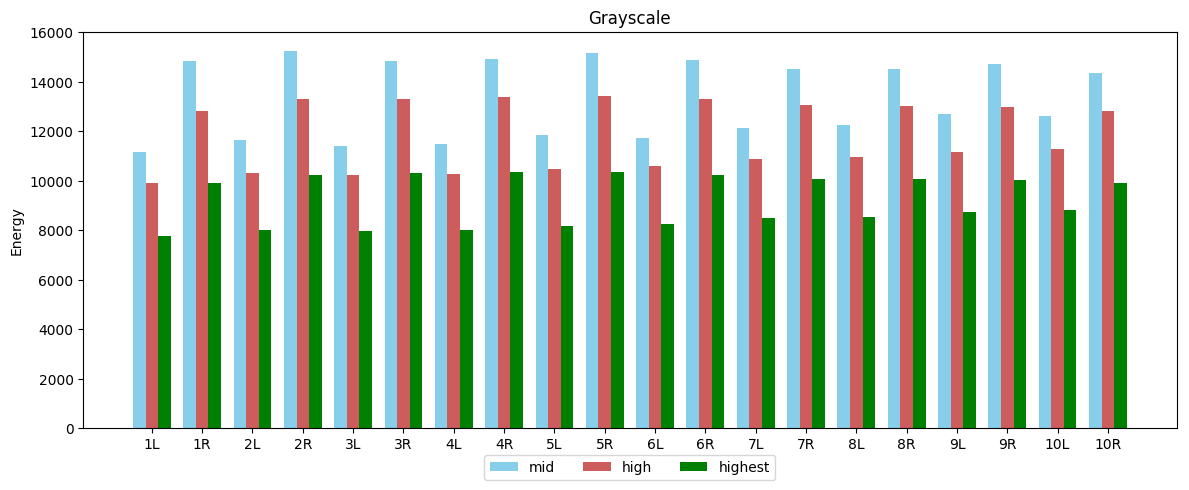
\includegraphics[scale=0.52, trim = {0 1cm 0 1cm}]{images/fig23.png}
% 	\end{center}
% 	\centering
%     \fautor
% \end{figure}

% \begin{figure}[ht]
% 	\centering
% 	\caption{\label{fig:stft_airplane}Grayscale colourspace STFT approach for airplane images.}
% 	\begin{center}
% 	    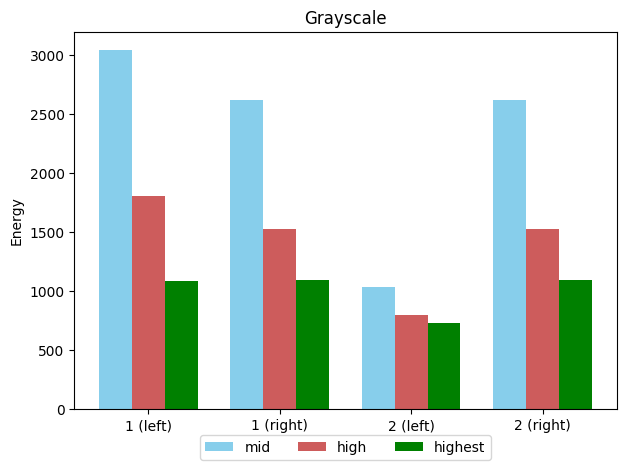
\includegraphics[scale=0.6, trim = {0 1cm 0 1cm}]{images/fig24.png}
% 	\end{center}
% 	\centering
%     \fautor
% \end{figure}

% \noindent The above graphs show that the magnitude of the energy levels on blurry sections is lower than the same metric for the non-blurry ones. Therefore, it provides evidence about the blur location. The most relevant results were obtained with the Grayscale and HSV colourspaces, such that neither the appendix \ref{chapter:fft-test-results} nor the \ref{chapter:stft-test-results} show the LAB results.

% \chapter{Conclusions}
% \label{chapter:conclusions}
% % From the preliminary results, it is possible to envisage and plan the activities to be done during the year of 2019 in order to achieve better performances and also better results. Preparations for the qualification exam and took consumed most of January and February. During this period, adjustments in the code were made and the necessity of some changes was noticed. These will be implemented and tested in March and April, together with the development of scientific articles with the proposed methods and results. After some changes in the code, improvements in the methods and evaluation of the tests, the new achievements should be summarized into the thesis; this will be done in May, June and July. More improvements may be done if needed during August and September, together with the article writing step. The last three months will be dedicated to prepare the thesis and to the defense. This schedule program is graphically represented in table \ref{tab:activity_schedule}:

% \begin{table}[H]
%     \caption{Activity schedule for 2019.}\label{tab:activity_schedule}
%     \begin{center}
%     \begin{tabular}{|c|c|c|c|c|c|c|c|c|c|c|c|c|}
%         \hline
   
%         & \multicolumn{6}{c|}{$1^{st}$ semester} 
%         & \multicolumn{6}{c|}{$2^{nd}$ semester}\\
%         \hline
   
%         & jan & feb & mar & apr & may & jun 
%         & jul & aug & sep & oct & nov & dec\\
%         \hline
        
%         Qualification
%         & \cellcolor{gray} & \cellcolor{gray} &  &  &  &  
%         &  &  &  &  &  & \\
%         \hline
        
%         Paper / Code
%         &  & \cellcolor{gray} & \cellcolor{gray} & \cellcolor{gray} &  & &  &  &  &  &  & \\
%         \hline
        
%         Paper / Thesis
%         &  &  &  &  & \cellcolor{gray} & \cellcolor{gray} & \cellcolor{gray} &  &  &  &  & \\
%         \hline
        
%         Paper / Code
%         &  &  &  &  & &  &  & \cellcolor{gray} & \cellcolor{gray} &  &  & \\
%         \hline
        
%         Thesis
%         &  &  &  &  & &  &  &  &  & \cellcolor{gray} & \cellcolor{gray} & \\
%         \hline
        
%         Defense
%         &  &  &  &  & &  &  &  &  &  &  & \cellcolor{gray}\\
%         \hline
%     \end{tabular}
%     \end{center}
%     \fautor
% \end{table}

% \chapter{Ferramentas úteis}
% \label{chapter:ferramentas-uteis}
% \input{tex/ferramentas-uteis}

% \chapter{Citações e referências}
% \label{chapter:citacoes}
% \input{tex/citacoes}


% ---
% Finaliza a parte no bookmark do PDF, para que se inicie o bookmark na raiz
% ---
\bookmarksetup{startatroot}% 
% ---

% ----------------------------------------------------------
% ELEMENTOS PÓS-TEXTUAIS
 ----------------------------------------------------------
\postextual

% ----------------------------------------------------------
% Referências bibliográficas
% ----------------------------------------------------------
\bibliography{references}

% ---------------------------------------------------------------------
% GLOSSÁRIO
% ---------------------------------------------------------------------

% Arquivo que contém as definições que vão aparecer no glossário
\input{tex/sections/glossario}
% Comando para incluir todas as definições do arquivo glossario.tex
\glsaddall
% Impressão do glossário
\printglossaries

% ----------------------------------------------------------
% Apêndices
% ----------------------------------------------------------

% ---
% Inicia os apêndices
% ---
% \begin{apendicesenv}

%     \chapter{FFT Results}
%     \label{chapter:fft-test-results}
%     \begin{figure}[htp]
    \caption{\label{fig:appendix_airplane_fft_results}Airplane FFT approach for (a) Grayscale, (b) HSV and (c) LAB images.}
    \centering
    \begin{subfigure}{.5\textwidth}
        \centering
        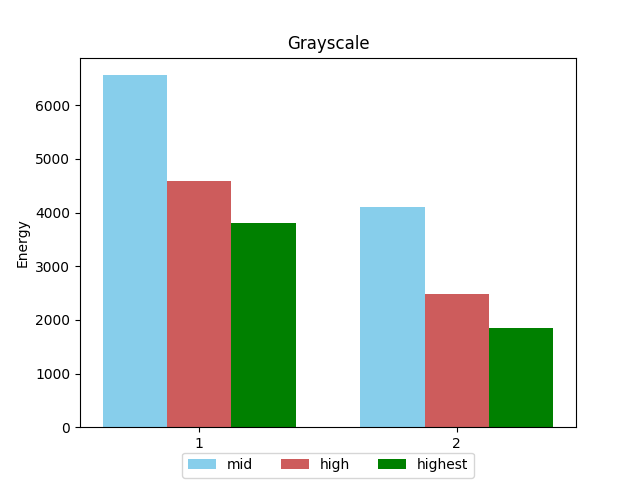
\includegraphics[scale=0.41]{images/appendix/fft/airplane/grayscale.png}
        \caption{}
    \end{subfigure}%
    \begin{subfigure}{.5\textwidth}
         \centering
          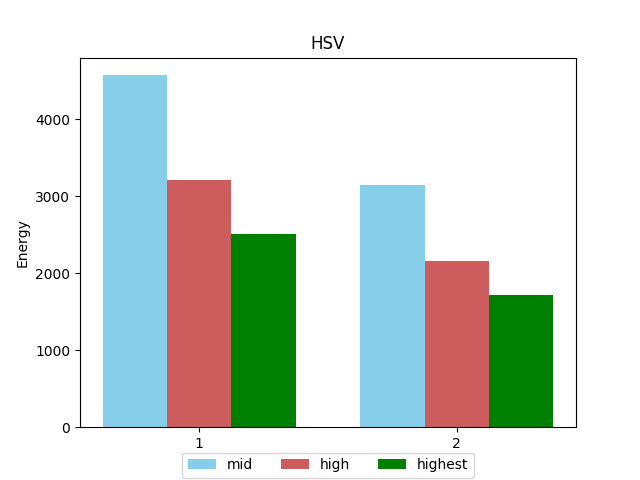
\includegraphics[scale=0.41]{images/appendix/fft/airplane/hsv.png}
          \caption{}
    \end{subfigure}
    \fautor
\end{figure}

\begin{figure}[H]
    \caption{\label{fig:appendix_card_fft_results}Card FFT approach for (a) Grayscale, (b) HSV and (c) LAB images.}
    \centering
    \begin{subfigure}{.5\textwidth}
        \centering
        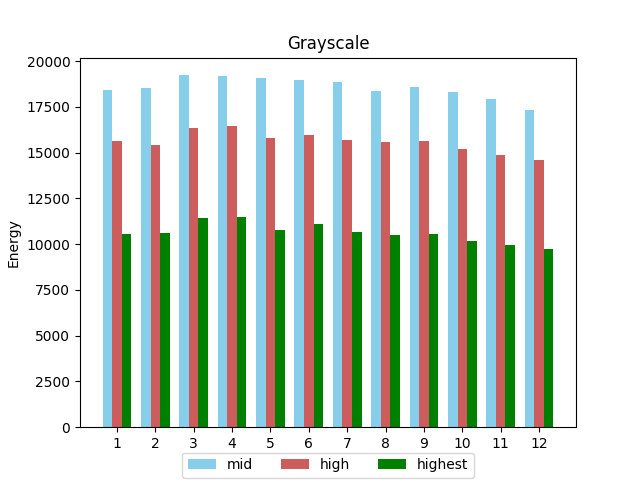
\includegraphics[scale=0.41]{images/appendix/fft/card/grayscale.png}
        \caption{}
    \end{subfigure}%
    \begin{subfigure}{.5\textwidth}
         \centering
          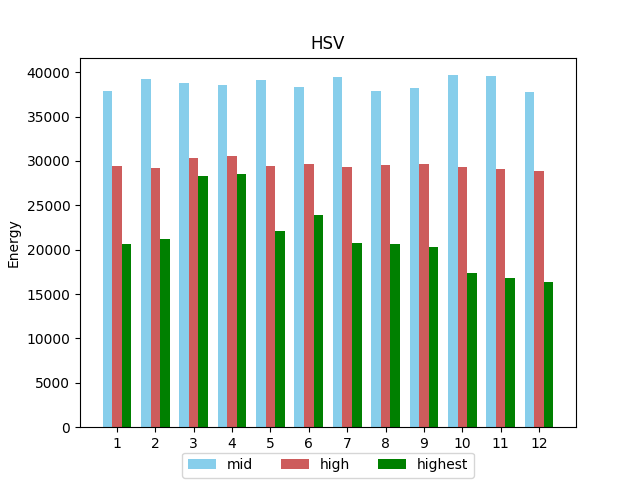
\includegraphics[scale=0.41]{images/appendix/fft/card/hsv.png}
          \caption{}
    \end{subfigure}
    \fautor
\end{figure}

\begin{figure}[H]
    \caption{\label{fig:appendix_coin_o_fft_results}Coin "o" letter FFT approach for (a) Grayscale, (b) HSV and (c) LAB images.}
    \centering
    \begin{subfigure}{.5\textwidth}
        \centering
        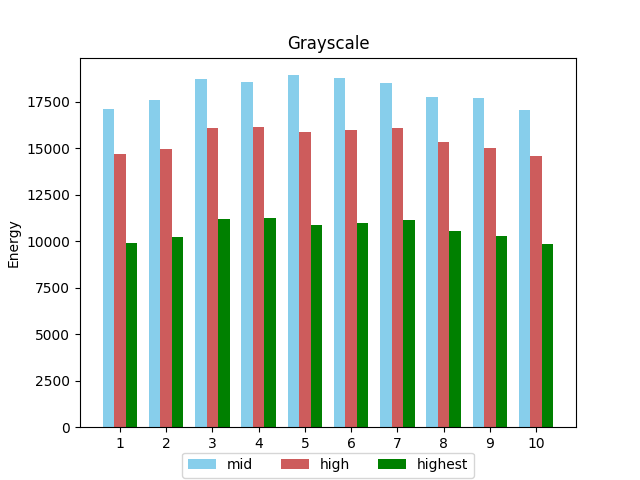
\includegraphics[scale=0.41]{images/appendix/fft/coin_o/grayscale.png}
        \caption{}
    \end{subfigure}%
    \begin{subfigure}{.5\textwidth}
         \centering
          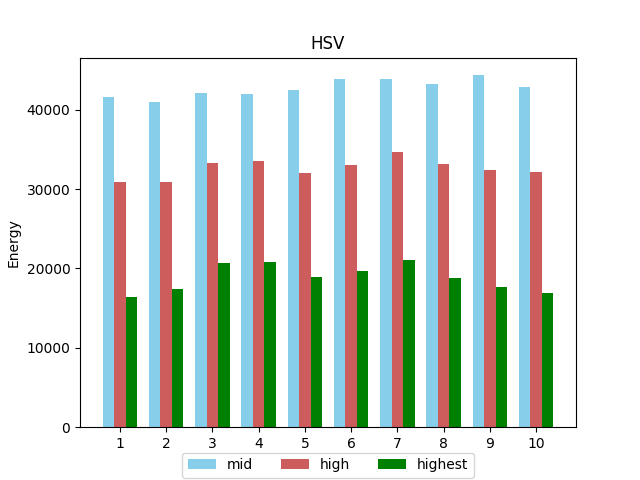
\includegraphics[scale=0.41]{images/appendix/fft/coin_o/hsv.png}
          \caption{}
    \end{subfigure}
    \fautor
\end{figure}

\begin{figure}[H]
    \caption{\label{fig:appendix_coin_v_fft_results}Coin "v" letter FFT approach for (a) Grayscale, (b) HSV and (c) LAB images.}
    \centering
    \begin{subfigure}{.5\textwidth}
        \centering
        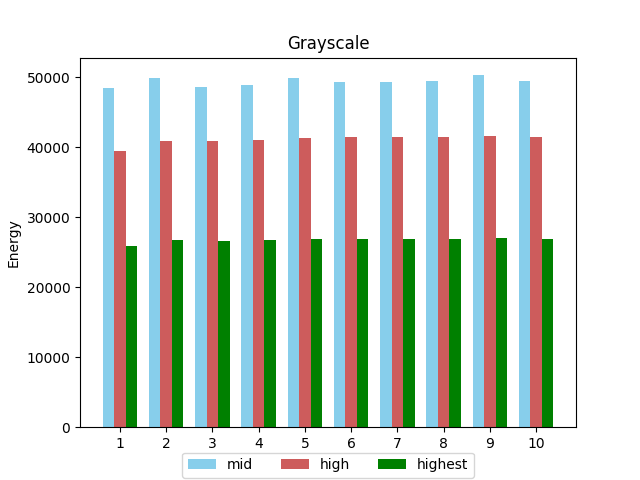
\includegraphics[scale=0.41]{images/appendix/fft/coin_v/grayscale.png}
        \caption{}
    \end{subfigure}%
    \begin{subfigure}{.5\textwidth}
         \centering
          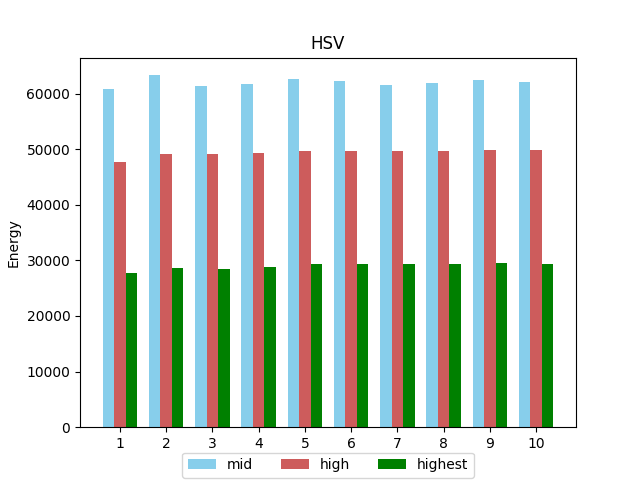
\includegraphics[scale=0.41]{images/appendix/fft/coin_v/hsv.png}
          \caption{}
    \end{subfigure}
    \fautor
\end{figure}

    
%     \chapter{STFT Results}
%     \label{chapter:stft-test-results}
%     \section{Hann Window}

\begin{figure}[!ht]
    \caption{Coin "o" STFT approach with Hann window for Grayscale (a) and HSV (b) colourspaces.}
    \centering
    \begin{subfigure}{\textwidth}
        \centering
        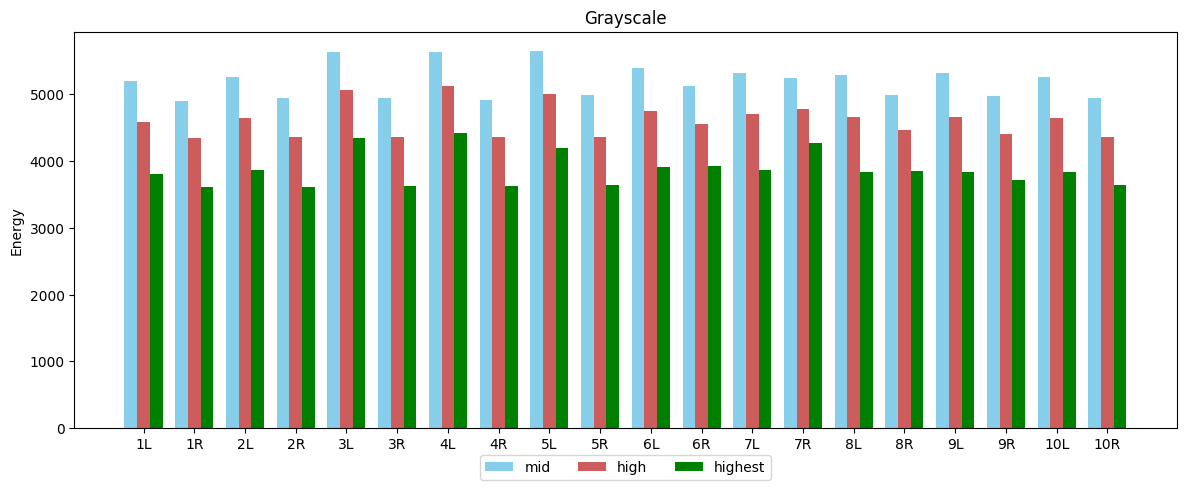
\includegraphics[scale=0.4]{images/appendix/stft/coin_o/hann_Grayscale.png}
        \caption{}
    \end{subfigure}\\
    \begin{subfigure}{\textwidth}
         \centering
          \includegraphics[scale=0.4]{images/appendix/stft/coin_o/hann_HSV.png}
          \caption{}
    \end{subfigure}
    \fautor
\end{figure}

\begin{figure}[H]
    \caption{Card STFT approach with Hann window for Grayscale (a) and HSV (b) colourspaces.}
    \centering
    \begin{subfigure}{\textwidth}
        \centering
        \includegraphics[scale=0.5]{images/appendix/stft/card/hann_Grayscale.png}
        \caption{}
    \end{subfigure}\\
    \begin{subfigure}{\textwidth}
         \centering
          \includegraphics[scale=0.5]{images/appendix/stft/card/hann_HSV.png}
          \caption{}
    \end{subfigure}
    \fautor
\end{figure}

\begin{figure}[H]
    \caption{Airplane STFT approach with Hann window for Grayscale (a) and HSV (b) colourspaces.}
    \centering
    \begin{subfigure}{.5\textwidth}
        \centering
        \includegraphics[scale=0.41]{images/appendix/stft/airplane/hann_Grayscale.png}
        \caption{}
    \end{subfigure}%
    \begin{subfigure}{.5\textwidth}
         \centering
          \includegraphics[scale=0.41]{images/appendix/stft/airplane/hann_HSV.png}
          \caption{}
    \end{subfigure}
    \fautor
\end{figure}


\begin{figure}[H]
    \caption{Coin "v" STFT approach with Hann window for Grayscale (a) and HSV (b) colourspaces.}
    \centering
    \begin{subfigure}{\textwidth}
        \centering
        \includegraphics[scale=0.5]{images/appendix/stft/coin_v/hann_Grayscale.png}
        \caption{}
    \end{subfigure}\\
    \begin{subfigure}{\textwidth}
         \centering
          \includegraphics[scale=0.5]{images/appendix/stft/coin_v/hann_HSV.png}
          \caption{}
    \end{subfigure}
    \fautor
\end{figure}

\section{Flattop Window}

\begin{figure}[H]
    \caption{Airplane STFT approach with Flattop window for Grayscale (a) and HSV (b) colourspaces.}
    \centering
    \begin{subfigure}{.5\textwidth}
        \centering
        \includegraphics[scale=0.41]{images/appendix/stft/airplane/flattop_Grayscale.png}
        \caption{}
    \end{subfigure}%
    \begin{subfigure}{.5\textwidth}
         \centering
          \includegraphics[scale=0.41]{images/appendix/stft/airplane/flattop_HSV.png}
          \caption{}
    \end{subfigure}
    \fautor
\end{figure}

\begin{figure}[!htb]
    \caption{Coin "o" STFT approach with Flattop window for Grayscale (a) and HSV (b) colourspaces.}
    \centering
    \begin{subfigure}{\textwidth}
        \centering
        \includegraphics[scale=0.4]{images/appendix/stft/coin_o/flattop_Grayscale.png}
        \caption{}
    \end{subfigure}\\
    \begin{subfigure}{\textwidth}
         \centering
          \includegraphics[scale=0.4]{images/appendix/stft/coin_o/flattop_HSV.png}
          \caption{}
    \end{subfigure}
    \fautor
\end{figure}

\begin{figure}[H]
    \caption{Card STFT approach with Flattop window for Grayscale (a) and HSV (b) colourspaces.}
    \centering
    \begin{subfigure}{\textwidth}
        \centering
        \includegraphics[scale=0.5]{images/appendix/stft/card/flattop_Grayscale.png}
        \caption{}
    \end{subfigure}\\
    \begin{subfigure}{\textwidth}
         \centering
          \includegraphics[scale=0.5]{images/appendix/stft/card/flattop_HSV.png}
          \caption{}
    \end{subfigure}
    \fautor
\end{figure}


\begin{figure}[H]
    \caption{Coin "v" STFT approach with Flattop window for Grayscale (a) and HSV (b) colourspaces.}
    \centering
    \begin{subfigure}{\textwidth}
        \centering
        \includegraphics[scale=0.5]{images/appendix/stft/coin_v/flattop_Grayscale.png}
        \caption{}
    \end{subfigure}\\
    \begin{subfigure}{\textwidth}
         \centering
          \includegraphics[scale=0.5]{images/appendix/stft/coin_v/flattop_HSV.png}
          \caption{}
    \end{subfigure}
    \fautor
\end{figure}

\section{Blackmanharris Window}

\begin{figure}[H]
    \caption{Airplane STFT approach with Blackmanharris window for Grayscale (a) and HSV (b) colourspaces.}
    \centering
    \begin{subfigure}{.5\textwidth}
        \centering
        \includegraphics[scale=0.41]{images/appendix/stft/airplane/blackmanharris_Grayscale.png}
        \caption{}
    \end{subfigure}%
    \begin{subfigure}{.5\textwidth}
         \centering
          \includegraphics[scale=0.41]{images/appendix/stft/airplane/blackmanharris_HSV.png}
          \caption{}
    \end{subfigure}
    \fautor
\end{figure}

\begin{figure}[H]
    \caption{Coin "o" STFT approach with Blackmanharris window for Grayscale (a) and HSV (b) colourspaces.}
    \centering
    \begin{subfigure}{\textwidth}
        \centering
        \includegraphics[scale=0.4]{images/appendix/stft/coin_o/flattop_Grayscale.png}
        \caption{}
    \end{subfigure}\\
    \begin{subfigure}{\textwidth}
         \centering
          \includegraphics[scale=0.4]{images/appendix/stft/coin_o/flattop_HSV.png}
          \caption{}
    \end{subfigure}
    \fautor
\end{figure}

\begin{figure}[H]
    \caption{Card STFT approach with Blackmanharris window for Grayscale (a) and HSV (b) colourspaces.}
    \centering
    \begin{subfigure}{\textwidth}
        \centering
        \includegraphics[scale=0.5]{images/appendix/stft/card/blackmanharris_Grayscale.png}
        \caption{}
    \end{subfigure}\\
    \begin{subfigure}{\textwidth}
         \centering
          \includegraphics[scale=0.5]{images/appendix/stft/card/blackmanharris_HSV.png}
          \caption{}
    \end{subfigure}
    \fautor
\end{figure}

\begin{figure}[H]
    \caption{Coin "v" STFT approach with Blackmanharris window for Grayscale (a) and HSV (b) colourspaces.}
    \centering
    \begin{subfigure}{\textwidth}
        \centering
        \includegraphics[scale=0.5]{images/appendix/stft/coin_v/blackmanharris_Grayscale.png}
        \caption{}
    \end{subfigure}\\
    \begin{subfigure}{\textwidth}
         \centering
          \includegraphics[scale=0.5]{images/appendix/stft/coin_v/blackmanharris_HSV.png}
          \caption{}
    \end{subfigure}
    \fautor
\end{figure}

% \end{apendicesenv}
% ---


% ----------------------------------------------------------
% Anexos
% ----------------------------------------------------------

% ---
% Inicia os anexos
% ---
% \begin{anexosenv}

%     \chapter{Páginas interessantes na Internet} 
%     \label{chapter:paginas-interessantes}
%     \begin{description}
 \item[\url{http://www.tex-br.org}] Página em português com diversos tutoriais e referências interessantes sobre \LaTeX;
 \item[\url{http://en.wikibooks.org/wiki/LaTeX}] Livro em formato \textit{wiki} gratuito sobre \LaTeX;
 \item[\url{http://tobi.oetiker.ch/lshort/lshort.pdf}] Ótimo tutorial sobre \LaTeX (possui versão em português \url{http://alfarrabio.di.uminho.pt/~albie/lshort/ptlshort.pdf}, mas a versão em inglês é a mais atual);
 \item[\url{http://code.google.com/p/abntex2/}] Página do abnTeX2, grupo que desenvolve os pacotes e classes em \LaTeX para as normas da ABNT, nos quais a classe \textit{icmc} foi baseada;
\item[\url{http://www.more.ufsc.br}] Página do Mecanismo On-line para Referências  (MORE) desenvolvido pela UFSC;
\item[\url{http://detexify.kirelabs.org/classify.html}] Página para recuperar o código de símbolos em \LaTeX a partir do desenho fornecido pelo usuário.
 \end{description}

% \end{anexosenv}
% ---

\end{document}